\documentclass[a4paper,12pt]{book}

\usepackage{a4}
\usepackage{isolatin1} 
\usepackage{amsmath,amsthm,amstext,amssymb,amscd} 
\usepackage{makeidx}
\usepackage{bbm}
\usepackage{epsfig} 
\usepackage{longtable}

\title{\textit{The MathletFactory Tutorial}}
\date{January 11th 2005}
\author{Markus Gronau, Tim Paehler}
\newcounter{figcount}
\newcommand{\appfac}{\emph{MathletFactory }}
\newcommand{\mmo}{\emph{MMObject }}
\newcommand{\mmos}{\emph{MMObjects }}
\newcommand{\mmp}{\emph{MMPanel }}
\newcommand{\mmps}{\emph{MMPanels }}
\newcommand{\op}{\emph{Operation }}
\newcommand{\ops}{\emph{Operations }}
\newcommand{\rel}{\emph{Relation }}
\newcommand{\R}{\mathbb{R}}
\newcommand{\Rtext}{$\mathbb{R}$ }
\newcommand{\Ztext}{$\mathbb{Z}$}
\begin{document}

\maketitle

\tableofcontents 

\chapter{General informations}

\section{What is the MathletFactory?}
  
  The \textit{MathletFactory} is a reusable component system for creating web-based 
  interactive mathematical applets (mathlets) which allows the rapid development 
  of such programs for instructional web systems.\\
  The \textit{MathletFactory} is part of the project MuMIE (http://www.mumie.net).\\\\
  Following the mathematical paradigm to separate logic from its representation, 
  it consists of both a mathematical library and a presentation and interaction 
  framework with an extensible event system.\\
  On the mathematical side it contains a large and still growing collection of 
  mathematical objects (up to now: number classes, matrices, polynomials, 
  vectorspaces, functions etc.) which give it a power almost compared to that of a 
  CAS. On the interactive side it allows users to place the mathematical objects 
  in different contexts and interactively change their state. By defining 
  dependencies between objects and update chains it allows learners to experience 
  mathematics at work simply by dragging objects (e.g. a vector point) or by 
  setting values from hand (e.g. values of a matrix) and watching the applet 
  dynamically displaying the new result.

\section{About this document}
  This document adresses to mathlet developers who wants to get familiar with the creation
  of mathlets using the MathletFactory's library. It does not aim to describe each
  single class but to illustrate the necessary techniques and philosophies for the 
  construction of a mathlet. This technical stuff will be accompanied by 
  comprehensive examples and hints. A complete overview of all classes can be found
  in the APIDOC. The use of the APIDOC will be assumed.

\section{Available resources}
  The MathletFactory library as well as the APIDOC, examples, sources and other
  documentation can be downloaded from the internet site:\\
  \indent\indent\indent\indent\indent\indent \textbf{http://www.mathletfactory.de}

\section{Setting up the environment}
  In order to compile and run java-applets you will need the Java Software Development Kit 
  (JDK/SDK) of (at least) version 1.4 as well as the Java3D-classes for 3D-Mathlets
  and the JavaMediaFramework (JMF) for screen capture support.\\
  For viewing applets in your internet browser, you will need a Java-plugin.\\
  All files can be downloaded for free from http://java.sun.com.\\
  The Java APIDOC and Java tutorial are also available there.
  \\\\
  You will need to put the MathletFactory library (JAR-file) into the java-classpath
  where the compiler and the runtime will search for the classes (see your 
  java-documentation for informations about setting the classpath).
  \\\\
  The use of a professional Integrated Development Editor (IDE) instead of a simple
  text editor is recommended. There you can include the APIDOC and the sources
  into the editor for an easier programming. 
  \\\\
  If you want to publish your own mathlets in the internet, you will need to 
  create a HTML-file where you can embed the applet (see Appendix) and to have 
  a copy of the MathletFactory-library on your server where the browser plugin 
  can find it.

\newpage

\chapter{Creating mathlets}

\section{First steps}
  \subsection{The choice of a mathlet type}
  The mathlet-class needs to extend one of the template classes below.
  There are mathlet template types for the most common needs. The main distinction
  of theses templates is made by the number, the arrangement and the dimension of 
  their canvases. \\
  The following template types are available:
  \begin{itemize}
    \item {\bf"No-Canvas"} -- none canvas and 1 ControlPanel\\
      \[NoCanvasApplet\footnote{net.mumie.mathletfactory.appletskeleton}\]
    \item {\bf"Single"} -- 1 single canvas and below 1 ControlPanel\\
      \[2D: SingleG2DCanvasApplet\footnote{net.mumie.mathletfactory.appletskeleton.g2d}, 
      3D: SingleJ3DCanvasApplet\footnote{net.mumie.mathletfactory.appletskeleton.j3d}\]
    \item {\bf"Side-By-Side"} -- 2 canvases arranged horizontally and below 1 ControlPanel\\
      \[2D: SideBySideG2DCanvasApplet^{2}, 3D: SideBySideJ3DCanvasApplet^{3}\]
    \item {\bf"Upper-Lower"} -- 2 canvases arranged vertically and below 1 ControlPanel\\
      \[2D: UpperLowerG2DCanvasApplet^{2}\]
    \item {\bf"Upper-Middle-Lower"} -- 3 canvases arranged vertically and below 1 ControlPanel\\
      \[2D: UpperMiddleLowerG2DCanvasApplet^{2}\]
  \end{itemize}
  The ControlPanel resides below the canvases, except for the
  \verb|NoCanvasApplet|: there it covers the whole mathlet's space.
  
  
  \subsection{Creating the applet class}
  The "entry point" of an applet is the \verb|init()| method which will be called
  by the web-browser to load and initialize the applet.\\
  An empty mathlet can look like this (e.g. for a "Single-Canvas"-applet):\\
  {\small\ttfamily
  \indent import net.mumie.mathletfactory.appletskeleton.g2d.*;\\\\
  \indent public class MyApplet extends SingleG2DCanvasApplet \{\\
  \indent ...\\
  \indent \indent public void init() \{\\
  \indent \indent \indent super.init() // needed to initialize the template\\
  \indent \indent\indent ... // your entry point\\
  \indent \indent \}\\
  \indent \}\\
  }
  Note that the call \verb|super.init()| is needed to initialize the super class.\\\\
  The browser plugin (or the appletviewer) needs a HTML page to start the applet.
  There the location to the compiled applet, its size and other parameters are defined.
  See \small{\textit{Appendix: Commands for embedding applets in websites}}.\\\\
  
  \subsection{Setting the title}
  The title is shown at top of the mathlet, above the canvases or the control panel.
  It can be set with\\
  \indent \verb|setTitle(String)|\\
  defined in the \verb|BaseApplet| class.
  
  \subsection{Implementing a {\tt main}-method}
  In order to start the mathlet as an application (i.e. outside the browser from the
  command line) you have to write:\\\\
  {\small\ttfamily
  \indent import ...\\
  \indent import net.mumie.mathletfactory.util.*;\\\\
  \indent public class MyApplet extends SingleG2DCanvasApplet \{\\
  \indent\indent ...\\
  \indent\indent public static void main(String[] args) \{\\
  \indent\indent\indent MyApplet applet = new MyApplet();\\
  \indent\indent\indent applet.init();\\
  \indent\indent\indent applet.start();\\
  \indent\indent\indent BasicApplicationFrame frame = \\
  \indent\indent\indent\indent\indent\indent new BasicApplicationFrame(applet, 400, 300);\\
  \indent\indent\indent frame.pack();\\
  \indent\indent\indent frame.setVisible(true);\\
  \indent\indent\}\\
  \indent\}\\
  }
  
\section{Using a Canvas}
  A canvas is a paint board where \mmos, images and text can be displayed. It can hold either 2- or 3-dimensional
  objects, their class is respectively \verb|MMG2DCanvas| or \verb|MMJ3DCanvas|, subclasses of \verb|MM2DCanvas| and
  \verb|MM3DCanvas|.\footnote{The distinction of two 2D and 3D canvas classes was made to allow in future releases
  the usage of other graphics implementations than the Java-proper ones (\textit{Graphics2D} and \textit{Java3D}).}
  The common class of these two different canvas types is \verb|MMCanvas|, where the biggest part of functionality
  is implemented.\\
  Objects can be added with\\
  \indent \verb|addObject(MMCanvasObjectIF|\footnote{net.mumie.mathletfactory.mmobject})\\
  defined in \verb|MMCanvas|\footnote{net.mumie.mathletfactory.display}.

\newpage
\section{Using a ControlPanel}
  The \verb|ControlPanel|\footnote{net.mumie.mathletfactory.appletskeleton.util} 
  represents a container for GUI(Graphical User Interface)-components,
  providing a flexible text editor-like layout manager. It allows the programmer 
  to add components and to lay out them in the mathlet as easy as writing a text: the
  ControlPanel's height will be divided upon all lines where each of them can have
  a different horizontal alignment (left, right and center). Their height is determined
  by the components's preferred sizes.\\
  At the begin (means no object has been added yet) a "line pointer" starts at the first
  line and adds all following components to it. A line will be terminated by a line
  break. The pointer will then jump to the second line.\\
  Note: No further adding and alignment setting will be possible for this line!\\
  It is possible to use tabstops and other space holders for exact positioning.
  \\\\
  The ControlPanel is a base functionality of the BaseApplet and all of its
  extending classes. In most cases it is positioned under the canvases (except for
  the NoCanvasApplet: there it fills the whole vertical space). It can be accessed
  through \verb|BaseApplet.getControlPanel()| or used indirectly by one of the delegate
  methods defined in the BaseApplet. These delegaters are named after their
  implementations in the ControlPanel, except the \verb|add()| method: its corresponding
  delegate method is \verb|addControl()|.\footnote{This distinction was made
  to show the difference between the add-method defined in the Applet-class
  and this one.}\\
  It is possible to create a new ControlPanel-instance (e.g. in a standalone applet
  or in a new tab) but it is not necessary to do this in the predefined mathlet
  classes.
  \\\\
  Method summary:
  \begin{itemize}
    \item \verb|add(JComponent)| -- adds a component to the actual line's end
    \item \verb|insertLineBreak()| -- jumps to the next line
    \item \verb|insertLineBreak(int)| -- jumps \verb|int| lines downwards
    \item \verb|insertTab()| -- inserts a single tabstop
    \item \verb|insertTab(int)| -- inserts \verb|int| tabstops
    \item \verb|insertHSpace(int), insertVSpace(int)| -- inserts place holders with \verb|int| pixels width/height
    \item sets the alignment of the actual and the following lines
    \begin{itemize}
      \item \verb|setLeftAlignment()| 
      \item \verb|setCenterAlignment()|
      \item \verb|setRightAlignment()|
    \end{itemize}
  \end{itemize}
  
\section{Using advanced BaseApplet functionality}
  
  \subsection{Structure of a mathlet}
  The BaseApplet defines a common design for all mathlets where the components
  are placed into predefined panels/panes (containers able to hold GUI-components).
  The 3 main panels of a mathlet are (read from top to bottom):
  \begin{itemize}
    \item title pane containing a label with the mathlet's title
    \item center pane containing the canvases and/or a control-panel
    \item button pane containing the help, reset, screenshot and animation buttons
  \end{itemize}
  The center pane itself is divided into (from top to bottom)
  \begin{itemize}
    \item canvas pane containing a single canvas or an arrangement of several canvases
    \item control-panel pane containing a ControlPanel
  \end{itemize}
  
  \subsection{Using Tabs}
    It is possible to open a new tab in the control-panel-, canvas- and center-pane.
    This is done by calling \verb|add(String, Component)| on the following getters:
    \begin{itemize}
      \item getCanvasTabbedPane()
      \item getCenterTabbedPane()
      \item getControlTabbedPane()
    \end{itemize}
  These methods return a customized instance of a JTabbedPane\footnote{javax.swing.JTabbedPane}
  (an instance of \verb|TabbedPanel| more precisly) which will show the real tab
  (with the tab's title) only when more than one tab has been added.\\
  Note: all of the BaseApplet's tabbed panes have allready a tab (containg the canvases, etc.).
  But the tab's titles are not visible because they are the only tabs!\\\\
  The add-method of these tabbed panes request a string for the tab's title and an
  instance of Component\footnote{java.awt.Component} which can be e.g. a new 
  ControlPanel, Canvas or JPanel (they all extends the class \verb|Component|).\\
  The title of the first (default) tab can be set through the \verb|TabbedPanel|-proper
  method \verb|setTitleAt(int, String)|. The instance of this underlying SWING-class
  can be accessed through \verb|getTabbedPane()| in the class \verb|TabbedPanel|.
  
  \subsection{Adding a reset button}
  The button itself can be added by simply calling \verb|addResetButton()| inside
  an extended BaseApplet-class. By pressing the button, the method 
  \verb|public void reset()| will be called in the mathlet. To react on this event
  you will have to overwrite this method in the applet-class.
  
  \subsection{Adding a screenshot button}
    The button will be visible when calling \verb|addScreenShotButton()| inside an
    extended BaseApplet-class.
  
  \subsection{Extending directly the {\tt BaseApplet}}
  Each {\tt BaseApplet} consists of several panels which are not yet added to the visible GUI (the
  {\it center}, {\it canvas} and {\it control pane}).
  Extending directly the {\tt BaseApplet} class means that this work has to been done explicitly.\\
  The biggest part of a {\tt BaseApplet} is the {\it center pane} which takes all the place between
  the title and the bottom bars. In a case of a so called "no-canvas-applet" the {\it center pane}
  has been added only a \emph{ControlPanel}. Note that each of theses panels in {\tt BaseApplet}
  is an extended version of \verb|JPanel| and \verb|JTabbedPanel|, allowing to show register cards
  only if more than 1 component has been added. Theses panels haves the additional identifier {\it tabbed}
  \footnote{In the case of the {\it center pane}, this and the {\it center tabbed pane} are exactly the same.}.
  In \verb|NoCanvasApplet| we have to write:\\
  \verb|    getCenterPane().add(getControlTabbedPanel());|\\\\
  In \verb|SingleG2DCanvasApplet| we have to write:
  \begin{footnotesize}
  \begin{verbatim}
    getCanvasTabbedPanel().add(getCanvasPane());
    getCanvasPane().setLayout(new BorderLayout());
    m_canvas = new MMG2DCanvas();
    getCanvasPane().add(m_canvas, BorderLayout.CENTER);
    getCanvasPane().add(getControlTabbedPanel(), BorderLayout.SOUTH);
    getCenterPane().add(getCanvasTabbedPanel());
  \end{verbatim}
  \end{footnotesize}
  
  \clearpage
  
\section{Using the MumieTheme}
  The MathletFactory uses an extended version of the Java SWING Metal-theme. It is used to
  retrieve default values for fonts and colors from a property-file.\\
  The class must be used in a static way, i.e. calling \verb|MumieTheme.DEFAULT_THEME| gets
  the actual single working instance of that class. Values can be retrieved through the various
  \verb|get|-methods.\\
  The default property files are located in the \verb|resource| folder of the distribution.
  It is possible to write its own files or to change the existing ones to manage its own
  default values.\\
  Due to the architecture of SWING, all properties should be (re-)loaded in the \verb|updateUI()| method
  of the corresponding SWING-class because after an update of the user interface, all dependant
  classes will reload their default properties from SWING.\\\\
  
  \subsection{Property Names}
  By default, each SWING component listens to various properties defining its font, color or
  border. Every property starts with the name of the component by omitting the "SWING-J" (i.e. "Button"
  instead of "JButton"), followed by a dot and the property type: "font", "background", etc.\\
  There also exist special properties for several \appfac classes (e.g. Canvas.background).
  
  \subsection{Fonts}
  A legal fonts declaration for the MumieTheme consists of 3 comma separated values: 
  font name, style and size.\\
  The font style is coded into the following strings: PLAIN, BOLD, ITALIC, BOLD-ITALIC.\\
  Example:\\
  \begin{verbatim}
    Button.font=Dialog,BOLD-ITALIC,12
  \end{verbatim}
  
  \subsection{Colors}
  A legal fonts declaration for the MumieTheme consists of three 3 comma separated color components 
  for red, green and blue (RGB).\\
  Example:\\
  \begin{verbatim}
    Button.background=230,230,230
  \end{verbatim}
  
  \clearpage

\section{Writing Help Files}
  \subsection{Default Help Files}
  By default, each mathlet comes along with a set of help files describing the base common
  functionality of each mathlet. The type of the mathlet (g2d, no-canvas, j3d) will be
  questioned to decide which default help files will be needed.\\
  The available files are located under \verb|resource/html|.
  
  \subsection{Individual Help Files}
  Each mathlet can have its own individual help file which must be a valid HTML file.
  If the applet parameter \verb|helpURL| was not set, the mathlet will try to search for its 
  help file with the following assumptions:
  \begin{itemize}
    \item the help file is located in the same directory as the mathlet or 
    \item in the subdirectory \verb|help| of the mathlet's directory
    \item the help file is named after the mathlet with the suffixes \verb|_info.html| or 
    \verb|_info_<locale>.html|
  \end{itemize}
  
  
  \subsection{Displaying Help Files}
  By default, each mathlet contains at the bottom left corner a {\it help} button opening
  the help for this mathlet.\\
  When the mathlet was started as an applet inside a web browser, it will try to
  open the help file inside a new browser window. If it was started as an application, no
  applet context is available so the mathlet will show the help file in an own window.
  Note that in this case the Java class \verb|JEditorPane|, responsible for displaying the file in the
  mathlet window, can only parse HTML 3.2. In case of a browser environment, the HTML version
  of the help file must be readable by the web browser.
  
  

\clearpage
%\usepackage[latin1]{inputenc}
%\usepackage{amsmath}
%\usepackage{amsfonts}
%\usepackage{amssymb}
%\usepackage[active]{srcltx} %for kdvi and kile
%\usepackage{epsfig}         %for the figures
%\usepackage{verbatim}       %for the comment-environment

%\newtheorem{example}{Example}

%\newenvironment{code}{\begin{verbatim}}{\end{verbatim}}
  
  
\section{Example: A triangle and its altitudes}
    We want to create an applet which draws a triangle with three moveable 
    points and computes the altitudes.
    
    \subsection*{The canvas}
      Generally for any visualization we need a so called "canvas" (or several 
      of them) to draw our objects of visualization. The \appfac for this 
      purpose provides different predefined canvases, such as a single or a 
      side-by-side canvas for both Graphics2D or Java3D applets. Any applet 
      therefore shall extend one of the abstract classes 
      \begin{itemize}
        \item \verb SingleG2DCanvasApplet ,
        \item \verb SideBySideG2DCanvasApplet ,
        \item \verb SingleJ3DCanvasApplet , or
        \item \verb SideBySideJ3DCanvasApplet . 
      \end{itemize}
      There is also an an applet skeleton for pure symbolic displaying with no 
      canvas, the \verb NoCanvasApplet .
      
    \subsection*{The methods init() and initializeObjects()}
      The method \verb init()  is called from the applet context (i.e. the browser or appletviewer) 
      or by a wrapper-main method (don`t forget, your applet won't work otherwise!). It calls at least 
      the method \verb initializeObjects(),  and adds all created 
      objects to the canvas.

      With an empty implementation,  we can already have a look at our efforts 
      (see below) until now. As can be seen, some control 
      icons are automatically added as well as a standard \mbox{"help"-button}. 
        \begin{footnotesize}
        \begin{verbatim}
import net.mumie.mathletfactory.appletskeleton.g2d.SingleG2DCanvasApplet;
import net.mumie.mathletfactory.util.BasicApplicationFrame;

public class TriangleAltitude extends SingleG2DCanvasApplet{
  
  public void init() {
    super.init();
    setTitle("Triangle Altitude Applet");
    initializeObjects();
  }
  
  protected void initializeObjects(){
  }

  public static void main(String[] args){
    TriangleAltitude myApplet = new TriangleAltitude();
    myApplet.init();
    BasicApplicationFrame f = new BasicApplicationFrame(myApplet,500);
    f.pack();
    f.setVisible(true);
  }
}
        \end{verbatim}
        \end{footnotesize}
        \begin{center}
	  \resizebox*{7cm}{!}{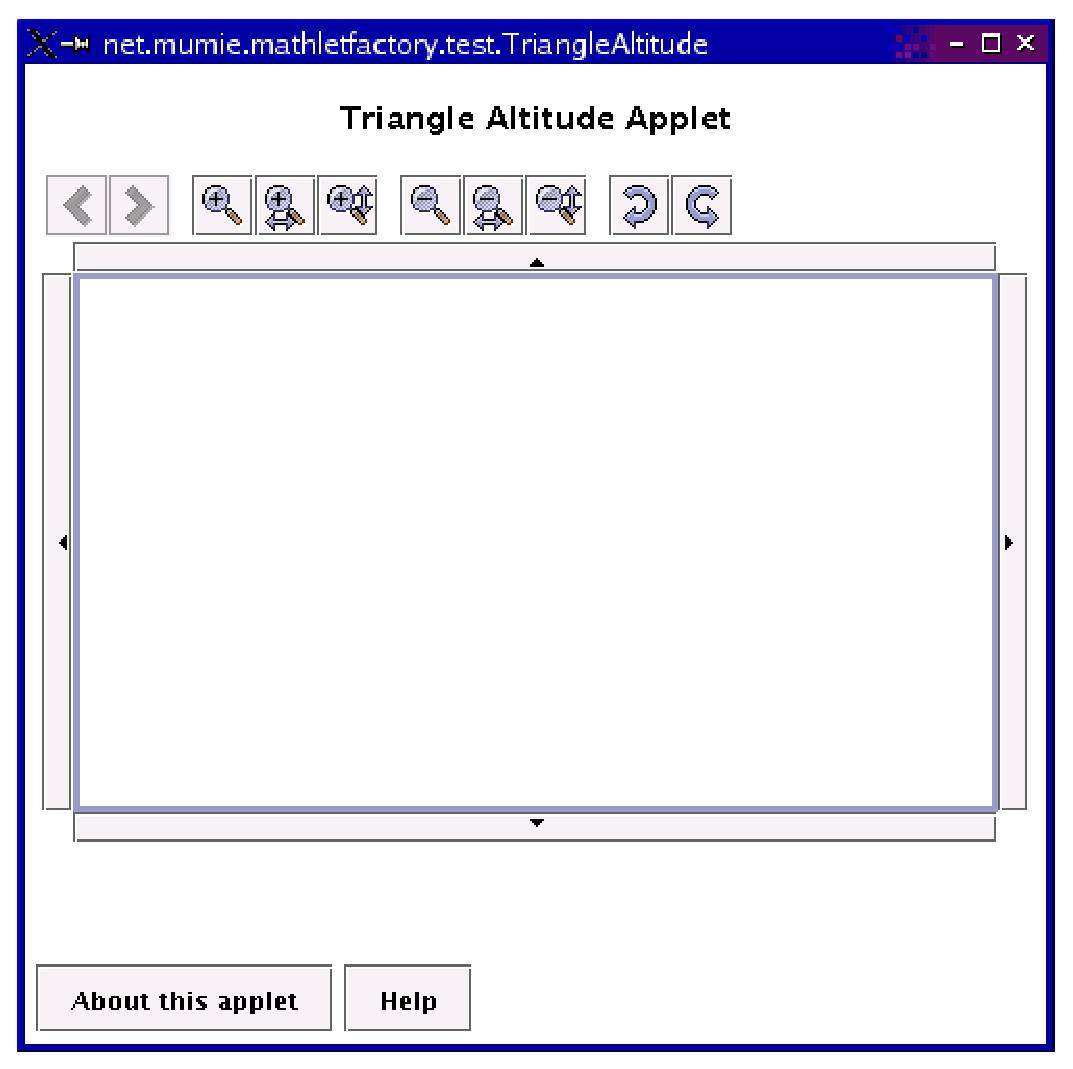
\includegraphics{images/triangleAltitudeFirst}}\\
        {\sf A single canvas applet.}\\
        \label{singlecanvas}
        \end{center}
    \subsection*{Number classes}
      Almost all objects are based on a so called number class like 
      \verb MDouble ,  \verb MRational ,  \verb MInteger ,  or 
      \verb MComplex .  They represent the real (with IEEE \verb double  precision), rational, natural, or complex 
      numbers. All computations are done within this class.
    \subsection*{Affine2DPoints}
      For the triangle we need three points A, B, C. They are realized by a so called 
      \verb MMAffine2DPoint  and defined by the representing number class and the coordinates:
      \begin{footnotesize}
      \begin{verbatim}
A = new MMAffine2DPoint(MDouble.class, -0.3, 0.3);
B = new MMAffine2DPoint(MDouble.class, 0.25, 0.25);
C = new MMAffine2DPoint(MDouble.class, -0.25, -0.25).
      \end{verbatim}
      \end{footnotesize}
      \vspace{-0.8cm}
    \subsection*{MouseTranslateHandler and KeyboardTranslateHandler}
      Since we want the points to be moveable by mouse and keyboard we create a
      so called \verb Affine2DMouseTranslateHandler  and an 
      \verb Affine2DKeyboardTranslateHandler  and add them to the points:
      \begin{footnotesize}
      \begin{verbatim}
amth = new Affine2DMouseTranslateHandler(getCanvas());
akth = new Affine2DKeyboardTranslateHandler(getCanvas());
A.addHandler(akth);     A.addHandler(amth);
B.addHandler(akth);     B.addHandler(amth);
C.addHandler(akth);     C.addHandler(amth);
      \end{verbatim}
      \end{footnotesize}
      \vspace{-0.8cm}
    \subsection*{Affine2DLineSegments}
      Now we need some line segments to connect the points of the triangle:
      \begin{verbatim}
AB = new MMAffine2DLineSegment(A,B);
BC = new MMAffine2DLineSegment(B,C);
CA = new MMAffine2DLineSegment(C,A).
      \end{verbatim}
      \vspace{-0.3cm}
      We also need line segments which represent the altitudes:
      \begin{verbatim}
altitude_AB = new MMAffine2DLineSegment(C,getPerpendicularFoot(A,B,C));
altitude_BC = new MMAffine2DLineSegment(A,getPerpendicularFoot(B,C,A));
altitude_CA = new MMAffine2DLineSegment(B,getPerpendicularFoot(C,A,B)).
      \end{verbatim}
      \vspace{-0.3cm}
      The method \verb getPerpendicularFoot()  returns a 
      \verb MMAffine2DPoint  representing the footpoint of the altitude.
      Some mathematical computation is
      done within this method which is not of interest for us now.

      Maybe the footpoint of an altitude does not lie on an edge of the 
      triangle. So we extend the edges by another line segment:
      \begin{footnotesize}
      \begin{verbatim}
aFootC = new MMAffine2DLineSegment(A,getPerpendicularFoot(A,B,C));
bFootC = new MMAffine2DLineSegment(B,getPerpendicularFoot(A,B,C));
bFootA = new MMAffine2DLineSegment(B,getPerpendicularFoot(B,C,A));
cFootA = new MMAffine2DLineSegment(C,getPerpendicularFoot(B,C,A));
cFootB = new MMAffine2DLineSegment(C,getPerpendicularFoot(C,A,B));
aFootB = new MMAffine2DLineSegment(A,getPerpendicularFoot(C,A,B)).
      \end{verbatim}
      \end{footnotesize}
      \vspace{-0.8cm}
      
%%%%%%%%%%%%%%%%%%%%%%%%%%%%%%%%%%%%%%%%%%%%%%%%%%%%%%%%%%%%%%%%%%%%%%%%%%%%%%%%%%%%%%%%%%%%%%%%
    \subsection*{Add objects to the canvas}
      Now all objects are created we have to add them to the canvas:\\\\
\begin{tabular}{l|l}
\begin{minipage}{6.5cm}
\begin{footnotesize}
\begin{verbatim}
getCanvas().addObject(A);
getCanvas().addObject(B);
getCanvas().addObject(C);

getCanvas().addObject(altitude_AB);
getCanvas().addObject(altitude_BC);
getCanvas().addObject(altitude_CA);
\end{verbatim}
\end{footnotesize}
\end{minipage}
&\begin{minipage}{6cm}
\begin{footnotesize}
\begin{verbatim}
getCanvas().addObject(AB);
getCanvas().addObject(BC);
getCanvas().addObject(CA);

getCanvas().addObject(aFootC);
getCanvas().addObject(bFootC);
getCanvas().addObject(cFootA);
getCanvas().addObject(cFootB);
getCanvas().addObject(aFootB);
getCanvas().addObject(bFootA);
\end{verbatim}
\end{footnotesize}
\end{minipage}
\end{tabular}
      
%%%%%%%%%%%%%%%%%%%%%%%%%%%%%%%%%%%%%%%%%%%%%%%%%%%%%%%%%%%%%%%%%%%%%%%%%%%%%%%%%%%%%%%%%%%%%%%%
    \subsection*{Display Properties}
      As can be seen in figure ??? all the lines and points have the standard 
      color black. If we want to give them another color we have to define
      \verb PointDisplayProperties   and \verb LineDisplayProperties  and set 
      them for the points and lines:
      \begin{footnotesize}
      \begin{verbatim}
private PointDisplayProperties pp = new PointDisplayProperties();
private LineDisplayProperties ll = new LineDisplayProperties();
private LineDisplayProperties mm = new LineDisplayProperties();
private LineDisplayProperties kk = new LineDisplayProperties();

\end{verbatim}
\end{footnotesize}
\begin{tabular}{l|l}
\begin{minipage}{7cm}
\begin{footnotesize}
\begin{verbatim}

pp.setObjectColor(Color.blue);
ll.setObjectColor(Color.red);
mm.setObjectColor(Color.red);
mm.setFilled(false);
kk.setObjectColor(Color.yellow);

A.setDisplayProperties(pp);
B.setDisplayProperties(pp);
C.setDisplayProperties(pp);

altitude_AB.setDisplayProperties(kk);
altitude_BC.setDisplayProperties(kk);
altitude_CA.setDisplayProperties(kk);

\end{verbatim}
\end{footnotesize}
\end{minipage}
&\begin{minipage}{6cm}

\begin{footnotesize}
\begin{verbatim}

AB.setDisplayProperties(ll);
BC.setDisplayProperties(ll);
CA.setDisplayProperties(ll);

aFootC.setDisplayProperties(mm);
bFootC.setDisplayProperties(mm);
bFootA.setDisplayProperties(mm);
cFootA.setDisplayProperties(mm);
cFootB.setDisplayProperties(mm);
aFootB.setDisplayProperties(mm);

\end{verbatim}
\end{footnotesize}
\end{minipage}
\end{tabular}
    
The result can be seen in figure ??. 

%%%%%%%%%%%%%%%%%%%%%%%%%%%%%%%%%%%%%%%%%%%%%%%%%%%%%%%%%%%%%%%%%%%%%%%%%%%%%%%%%%%%%%%%%%%%%%%%
    \subsection*{Dependency}
      Now our points are moveable but the lines do not move with them. 
      Obviously the position of the lines depend on the position of the points.
      This is described by a so called \verb DependencyAdapter  and the 
      method \verb dependsOn().  For example for the edges of the triangle we 
      have
      \begin{footnotesize}
      \begin{verbatim}
DependencyAdapter DPA = new DependencyAdapter() {
  public void doUpdate(MMObjectIF dependant, MMObjectIF[] free) {
    MMAffine2DLineSegment line = (MMAffine2DLineSegment) dependant;
    line.setInitialPoint((MMAffine2DPoint)free[0]);
    line.setEndPoint((MMAffine2DPoint)free[1]);
  }
};
AB.dependsOn(new MMObjectIF[]{A,B},DPA);
BC.dependsOn(new MMObjectIF[]{B,C},DPA);
CA.dependsOn(new MMObjectIF[]{C,A},DPA);
      \end{verbatim}
      \end{footnotesize}
      \vspace{-0.3cm}
      Hereby the first argument \verb new  \verb MMObjectIF[]{A,B}  of the 
      method \verb dependsOn()  is an array of objects on which the object 
      \verb AB  depends. This array is passed to the 
      method \verb doUpdate  in the \verb DependencyAdapter  \verb DPA  as 
      parameter \verb free.  \verb AB  is passed to the 
      method \verb doUpdate  in the \verb DependencyAdapter  as parameter 
      \verb dependent.  \verb doUpdate  describes the action to perform when
      an object of the array \verb free  is changed.
    \subsection*{Reset, Screenshot, About this applet button}
      With the commands
      \begin{verbatim}
addResetButton();
addScreenShotButton();
      \end{verbatim}
      \vspace{-0.3cm}
      we can add a reset and a screenshot button. The functionality of the 
      reset button is defined in the method \verb reset(),  which calls the 
      method \verb initializeObjects()  and repaints the canvas:
      \begin{footnotesize}
      \begin{verbatim}
public void reset(){
  initializeObjects();
  getCanvas().renderScene();
  getCanvas().repaint();
}.
      \end{verbatim}
      \end{footnotesize}
      \vspace{-0.3cm}
    A HTML-description of the functionality of the applet can be saved in a 
    file with the name \verb <class_name>_info.html. This desciption is opend 
    in another window by clicking the about-this-applet button.\\

    \begin{center}
	\resizebox*{6cm}{!}{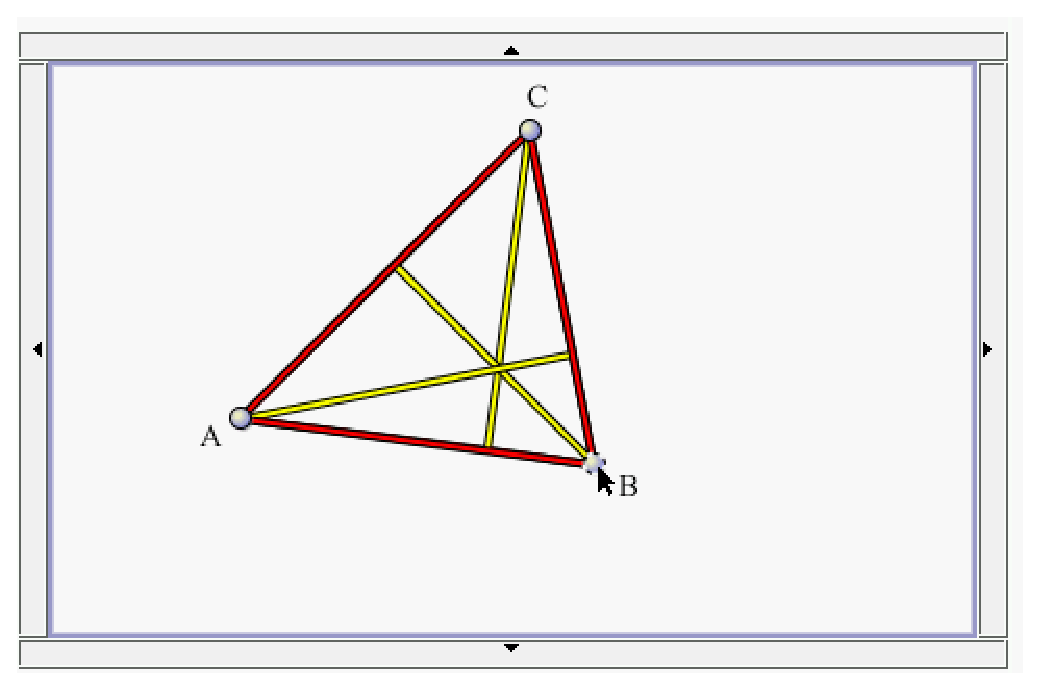
\includegraphics{images/triangle_altitudes}}\\
	{\sf The completed applet}
    \end{center}
    Now our first applet is ready. The full program can be found in the Appendix (TriangleAltitude).

%%%%%%%%%%%%%%%%%%%%%%%%%%%%%%%%%%%%%%%%%%%%%%%%%%%%%%%%%%%%%%%%%%%%%%%%%%%%%%%%%%%%%%%%%%%%%%%%
	\subsection*{Summary: Building Mathlets}
	\label{building_mathlets}
	These examples should illuminate the process of rapid applet development. The linear process 
	model we used can be generalized to the following steps:
	
	\begin{enumerate}
	\item Choose the display type and numbers of displays to be used and extend the corresponding applet skeleton.
	\item Add the chosen mmobjects and their iconic or symbolic representations
	\item Add necessary handlers
	\item Create the update graph by adding updaters and creating dependencies
	\end{enumerate}


\clearpage


  
\chapter{MMObjects}

\section{Introduction}
  \mmos (Multimedial Mathematical Objects) are the primary entities with which 
  an application programmer of the MathletFactory has to deal with. The MathletFactory 
  tutorial gives an overview of the framework that provides the simple use of \mmos. 
  This can be summarized in one sentence: \mmos encapsulate the mathematical and 
  interactivity state and are mapped onto graphic primitives (so called {\it drawables}) 
  and panel representation (so called {\it MMPanels}) by the use of specialised 
  {\it transformers}.\\
  An \mmo is either a super class of a mathematical class\\(located in \verb|net.mumie.mathletfactory.math|)
  implementing the \verb|MMObjectIF| interface or an extension of the class \verb|MMDefaultCanvasObject|
  or \verb|DefaultMMObject|, implementing 
  itself this interface and its necessary methods.\\
  Note: \\
  \begin{itemize}
    \item -- every \mmo's name starts with the two capital letters "MM"
    \item -- every \mmo is located in the tree branch \verb|net.mumie.mathletfactory.mmobject|
  \end{itemize}
  
  
\section{Displaying MMObjects}
  A single \mmo can be displayed in multiple instances of container- and canvas drawables.
  (a "Container" means a box where GUI-elements such as buttons, labels and textfields
  can be added and displayed)(e.g. the \verb|ControlPanel| or a simple \verb|JPanel|).\\
  Thereby it is possible to display the \mmo's content for different transform types
  in separate drawables and even in multiple instances for the same type.
  
 \subsection{Representing content in Containers}
    Each time one of the methods
     \begin{itemize}
      \item getAsContainerContent()
      \item getAsContainerContent(int)
    \end{itemize}
    is called, a new container drawable instance is created and returned. The first
    method returns the default container drawable, the second the drawable designated
    by the transform type. It is necessary to store it in a variable because these
    methods will never return this same instance again. The returned component can
    then by casted to the drawables runtime class to gain access to class-specific 
    functionality.
  
  \subsection{Representing content in Canvases}
    Each time one of the methods
     \begin{itemize}
      \item getAsCanvasContent()
      \item getAsCanvasContent(int)
    \end{itemize}
    is called, a new container drawable instance is created and returned. The first
    method returns the default container drawable, the second the drawable designated
    by the transform type. It is necessary to store it in a variable because these
    methods will never return this same instance again. The returned component can
    then by casted to the drawables runtime class to gain access to class-specific 
    functionality.
    
  \subsection{Display Properties}
  Each \mmo has its own display properties which define appearance related settings such as colors,
  fonts or transparency. They can be returned and set with
  \begin{itemize}
    \item \verb|getDisplayProperties()|
    \item \verb|setDisplayProperties(DisplayProperties)|
  \end{itemize}
  Both methods are defined in the interface \verb|MMObjectIF|.\\
  Moreover some MM-classes have extended properties where special settings are
  possible. By casting to the \verb|DisplayProperties|-runtime class they offer additional methods to
  change other useful settings such as the line width, point radius or the basic shape of a drawable:\\
  \begin{footnotesize}
  \begin{verbatim}
  MMAffine2DPoint p1;
  // ... initializing the point ...
  PointDisplayProperties pdp = (PointDisplayProperties)p1.getDisplayProperties();
  pdp.setPointRadius(10);
  \end{verbatim}
  \end{footnotesize}
  Sometimes we want to have 2 identical display properties, except 1 setting. Avoid such code:\\
  \begin{footnotesize}
  \begin{verbatim}
  DisplayProperties dp1 = new DisplayProperties();
  DisplayProperties dp2 = dp1; (*)
  dp1.setTransparency(0.25);
  dp2.setTransparency(0.75); // dp1 will be changed!
  \end{verbatim}
  \end{footnotesize}
  It is possible to call \verb|clone()| on an instance of \verb|DisplayProperties| to copy the settings
  into a new independant instance. The line (*) must be:\\
  {\small\ttfamily
    DisplayProperties dp2 = dp1.clone();\\
  }
  \\See \small{\textit{Appendix: Usage of DisplayProperties in \mmos and Drawables}}
  for a list of available properties-classes and their implementing \mmos and 
  the drawables using them.  
  
  
\section{Rendering cycle}
  Each rendering cycle is started either by a canvas, by the mathlet author (calling a manual repaint on the \mmo with 
  the \verb|render()| method) or by a handler (calling itself the \verb|render()| method).\\
  The \mmo forwards the repaint request to all of its working transformers which will set the internal data
  of the \mmo's drawables accordingly to the actual mathematical content.\\
  Calling \verb|render()| on a \mmo is therefore equivalent to calling \verb|render()| on every transformer
  instance hold by the \mmo.\\
  \\
  Example: 2D point\\
  The \verb|MMAffine2DTransformer| gets the coordinates of its "master" (here: \verb|Affine2DPoint|) and passes 
  them to its drawable (here: \verb|G2DPointDrawable|) which will draw a point at the new coordinates in the canvas.\\
  When dragging the point with the mouse, an instance of the class \verb|Affine2D|\-\verb|MouseTranslateHandler| will set 
  the new coordinates in the master (a \verb|MMAffine2DPoint|) and the rendering cycle will continue
  as described above.
  
  
\section{Number class}
  Most \mmos (or maybe their underlying mathematical classes) are dependant of a number type,
  means calculations are made through the number-class-proper arithmetic operations/methods.\\
  All MM-classes need this number class as parameter for their constructors for initializing their
  internal fields with numbers of this class. A change of the class outside the constructor (i.e. after
  initializing) is generally not possible.\\
  The available number classes are (located in \verb|net.mumie.mathletfactory.math.number|):\\
  {\ttfamily
    MDouble, MComplex, MRational, MComplexRational, MBigRational, MInteger, MNatural, MRealNumber, Zmod5.\\
  }
  
\section{Adding new MMObjects}
  
This document gives a brief overview of how to add user defined \mmos to the MathletFactory. This is done in three steps: 
Extending the {\tt MMDefaultCanvasObject}, implementing the associated transformer(s) and registering the \mmo-transformer 
mapping in the specific transformer.properties file(s).
  
\subsection{Introduction}
\mmos are the primary entities with which an application programmer of the MathletFactory has to deal with. The MathletFactory 
tutorial gives an overview of the framework that provides the simple use of \mmos. This can be summarized in one sentence: \mmos
encapsulate the mathematical and interactivity state and are mapped onto graphic primitives (so called {\it drawables}) and panel 
representation (so called {\it MMPanels}) by the use of specialised {\it transformers}.

\subsection{Extending the {\tt MMDefaultCanvasObject}}
Writing a \mmo usually starts by implementing a subclass of the {\tt MMDefaultCanvasObject}
class\footnote{\mmos with no graphical representation can use instead the class {\tt MMDefaultObject} which represents a \mmo with 
only a symbolic representation}. This class provides already 
the base functionality for handling the interactivity state (handlers, updaters, dependencies), therefore only the mathematical state 
has to be implemented. An alternative approach would be to extend one of the mathematical classes by implementing the 
{\tt MMCanvasObjectIF} interface. This was, for example, done in the implementation of some \mmos representing affine geometric 
entities (points, lines, etc.).\\
The abstract methods to be implemented when extending\\ {\tt MMDefaultCanvasObject} are the two following:\\

\begin{description}
\item[{\tt getDefaultTransformType()}]
Should return one of the transform types specified as constant in the class 
{\tt GeneralTransformer}. As may be guessed, this value is important for determining the correct transformer for the 
\mmo when invoking the methods\\ {\tt MMDefaultCanvasObject.getAsContainerContent()} and\\
{\tt MMDefaultCanvasObject.getAsCanvasContent()}.\\
 
\item[{\tt getNumberClass()}] 
This method implements the number class used by the \mmo. This must be one of the subclasses
of {\tt MNumber} and specifies, whether the mathematical entity bases on integer, rational, real, etc. numbers. The number 
class is needed for initializing all \mmos, a change after initialization is usually
not possible.
\end{description}

\subsection{Implementing the Transformer}
The transformer offers functionality responsible for the rendering, i.e. the mapping of \mmos onto graphical primitives 
(drawables) or panel representations (MMPanels). Note that it does not implement the actual graphical representation itself but keeps 
it as a reference and updates its configuration according to the \mmo's state. This allows it to reuse graphical primitives for 
a wide range of \mmos.\\
For allowing sophisticated geometry rendering, the MathletFactory offers a two level rendering approach using Math coordinates, world
coordinates and screen coordinates with the appropriate transformation functions {\tt math2World} and {\tt math2Screen}. However, for 
simple (usually affine) rendering, only one of these transformations has to be specified other than the identity.\\
Corresponding to the different rendering subsystems, there are three different types of transformers. The G2D transformers (located 
in the subpackage {\tt transformer.g2d}) perform rendering for 2D representations using the Java2D api, the J3D transformers (located 
in the subpackage {\tt transformer.j3d}) perform rendering for 3D representations using the Java3D api and the NOC (=No Canvas) 
transformers (located in the subpackage {\tt transformer.noc}) perform rendering onto Components.\\
Provided the drawable or MMPanel exists, implementing a transformer is quite straightforward and can be done by copying an existing
transformer and editing a few methods. These methods differ with the type of the transformer and are listed in the following
subsections:

\subsubsection{G2D Transformers}
For G2D Transformers, extending the class {\tt Affine2DDefaultTransformer} offers a good starting point. Besides the constructor, 
where the drawables are specified (see below), the following methods need to be implemented:
\begin{description}
\item[{\tt synchronizeMath2Screen()}] This method is used for rendering the mathematical state directly onto the screen.
 
\item[{\tt synchronizeWorld2Screen()}] This method is used for rendering the world coordinates (already calculated from the 
mathematical state) onto the screen. This method is usually invoked by {\tt synchronizeMath2Screen()} after {\tt math2World}
transformation has been performed.
\end{description}

\subsubsection{J3D Transformers}
For J3D Transformers, extending the class {\tt Affine3DDefaultTransformer} offers a good starting point. Besides the constructor, 
where the drawables are specified (see below), the following methods need to be implemented:
\begin{description}
\item[{\tt synchronizeMath2Screen()}] This method is used for rendering the mathematical state. As the actual representation on
the screen depends on the viewers position, this method should only implement the transformation from mathematical state to 
resulting world coordinates, leaving the projection on the screen to the 3D rendering system.
 
\item[{\tt getWorldPickPointFromMaster()}] This method should return a 3D point, that might act as a `center of gravity' when 
determining the medium distance of the drawable from the viewer. 
\end{description}

\subsubsection{NOC Transformers}
For NOC transformers, the class {\tt ContainerObjectTransformer} should be extended, representations using matrices may be 
derived from\\ {\tt TransformerUsingMatrixPanel}. The following methods need to be implemented:
\begin{description}
\item[{\tt initialize(MMObjectIF master)}] This method is used for creating the MMPanel, handing it over the master \mmo
needed for call-backs (e.g. editing of entries).
\item[{\tt render()}] This method is used for rendering the mathematical state directly onto the screen. Note that unlike in the
canvas transformers, where rendering does not include the actual drawing of the object (this is done by the canvas), this 
method should contain a {\tt repaint()} call for the MMPanel after transferring the mathematical state.
\end{description}

\subsection{Using and Referencing Drawables in {\tt CanvasTransformers}}
Since an \mmo transformed by a single transformer may have multiple drawables (e.g. a cuboid would be displayed by using
multiple rectangles), some of which may be active or inactive (e.g. a line would be either rendered by a line drawable or 
- in the degenerated case - by a point drawable), the developer has to specify the type of drawables needed by the Transformer.
The {\tt CanvasTransformers} class therefore offers support for multiple types of drawables, the following is an excerpt from 
its source code:

\begin{footnotesize}
\begin{verbatim}
  /**
   * this array holds all possible {@link ...CanvasDrawable}s
   * necessary to visualize the mathematics
   */
  protected CanvasDrawable[] m_allDrawables;

  /**
   * this array holds additional <code>CanvasDrawables</code> that might be
   * required by the &quot;real&quot; mathematics. Here we think of extra
   * presentation of boundary values for functions defined on borel sets
   * (these might be displayed as point objects, whereas the actual function
   * graph is displayed as a polygon) etc.
   */
  protected CanvasDrawable[] m_additionalDrawables;

  /** If a drawable is contained in this set, it neither rendered, nor drawn. */
  protected Set m_invisibleDrawables = new HashSet();

  /**
   * this will be the instance of the current active (valid)
   * <code>CanvasDrawable</code> and always points to one of the drawables
   * stored in {@link #m_allDrawables}.
   */
  protected CanvasDrawable m_activeDrawable;
\end{verbatim}
\end{footnotesize}
Since the fields are used in various methods, they should be initialized in the constructor.

\subsection{Registration of the MMObject-Transformer Mapping}
After the transformer has been constructed, it needs to be registered for a chosen transform type and in a specific display.
This is done by adding an entry to the {\tt transformer.properties.g2d}, {\tt transformer.properties.j3d} or  
{\tt transformer.properties.noc} file (depending on the type of the transformer), located in the transformer package. This 
entry is of the following form:\\
{\footnotesize\tt <transform type>\#<screen type>\#<mmobject class>=<transformer class>}\\ 
where {\tt transform type} is either the default transform type of the \mmo or the argument specified in the 
{\tt getAsCanvasContent(int transformType)} or {\tt setCanvasTransformer(int transformType, int screenType)} call creating the 
transformer and {\tt screen type} is {\tt ST\_GRAPHICS2D}, {\tt ST\_J3D} or {\tt ST\_NO\_CANVAS}. The possible values for
both of these variables are constants defined in the {\tt GeneralTransformer} class.
  
\chapter{Interactivity}
  \section{Dependencies}
  Sometimes a MM-object needs for its calculations the values of other objects.
  This implies that it must be recalculate its value whenever its "parameters"
  (i.e. the other objects) change to be up-to-date.\\
  It is possible to define relations between MM-objects so that one of them is dependant
  of the others. When one of the later is changed, the depending object will be
  updated. This can be done be implementing all 3 methods defined in the 
  \verb|DependencyIF|-interface
  {\small\ttfamily
  \begin{itemize}
    \item doUpdate()
    \item doUpdate(MMObjectIF dependant, MMObjectIF free)
    \item doUpdate(MMObjectIF dependant, MMObjectIF[] free)
  \end{itemize}
  }
  or by overwriting one of the methods of the
  \verb|DependencyAdapter|-class (which implements the interface with empty methods).
  The later possibility is recommended because it is sufficient to use only 1 of them: 
  all 3 methods will be called one after the other during one update cycle.
  Using the interface will cause to implement 2 methods with an empty body.\\
  After the \textit{doUpdate}-method has been called, the \textit{dependant} object
  will be rendered.
  \\\\
  Say we have 3 MM-objects named \textit{dependant, free1, free2} and we want the
  \textit{dependant} to calculate its value if one of the free-objects changes its
  value:\\
  {\small\ttfamily
  \begin{verbatim}
  MMObjectIF dependant, free1, free2;
  ... //initialize the fields above
  dependant.dependsOn(new MMObjectIF[] {free1, free2},
      new DependencyAdapter() {
        public void doUpdate() {
          ... // calculate
        }
      }
  );
  \end{verbatim}
  }
  If the MM-objects involved in this update are NOT known in the \textit{doUpdate}-method
  (i.e. the adapter-class is used for many dependencies) the passed MM-objects
  must be casted to their original class to use the full functionality of the
  MM-class.
  \\\\
  {\bf Example:} line segment between 2 points\\
  We want to create a line between 2 points that listens to changes of its start- and endpoint.
  The \textit{dependant} wourld be a \verb|MMAffine2DLineSegment| and the 2 \textit{free}-objects
  instances of \verb|MMAffine2DPoint|:\\
  {\small\ttfamily
  \begin{verbatim}
  import net.mumie.mathletfactory.mmobject.geom.affine.*;
  import net.mumie.mathletfactory.action.updater.DependencyAdapter;
  ...
  MMAffine2DLineSegment line1, line2;
  MMAffine2DPoint start1, start2, end1, end2;
  ...
  DependencyAdapter lineAdapter = new DependecyAdapter() {
    public void doUpdate(MMObjectIF dependant, MMObjectIF[] free) {
      MMAffine2DLineSegment line = (MMAffine2DLineSegment) dependant;
      MMAffine2DPoint p1 = (MMAffine2DPoint)free[0];
      MMAffine2DPoint p2 = (MMAffine2DPoint)free[1];
      line.setInitialPoint(p1);
      line.setEndPoint(p2);
    }
  };
  line1.dependsOn(new MMObjectIF[]{start1, end1}, lineAdapter);
  line2.dependsOn(new MMObjectIF[]{start2, end2}, lineAdapter);
  ...
  \end{verbatim}
  }
  
  \section{Updaters}
  
  \section{Animations}
    Animations allow a succession of actions during a defined duration.
    They are defined by one or many steps defining themselves the "real"
    actions. The steps's order is determined by the order the steps have been added
    to the animation (FIFO principle).
    Successive actions should be grouped into separate steps where a better control
    of initializations between two successive actions can be reached.
    Actions which are dependant of the step's progress (e.g. dragging an object
    from one position to another) must be made to process a number between zero
    (begin)(0%) and 1 (end)(100%). There are 2 possiblities to 
    
    \subsection{Creating steps}
    An animation step is created with a \textit{long}-value as duration or with a
    second parameter, the call count as an \textit{int}-number.
    \\\\
    The animating calcuation part is done by the \textit{proceed(Progress)}-method which
    must be overwritten by 
    
    \subsection{Using animation-dependencies}
      Animation-dependencies work similiarly to the "normal" depedencies except that
      the \textit{doUpdate}-methods have a third argument: the progress.
      
    \subsection{Displaying the controls}
      The components available to control an animation are:
      \begin{itemize}
        \item the {\it button panel} with the main control buttons: {\tt getButtonPanel()}
        \item the {\it description label} with the currently displayed message: {\tt getDescriptionLabel()}
        \item the {\it options panel} for changing settings: {\tt getOptionsPanel()}
      \end{itemize}
      These 3 components are grouped into the {\it animation panel}: {\tt getAnimationPanel()}
      \\\\
      It is possible to place the {\it button panel} into the bottom bar of the mathlet,
      between the {\it help- and reset-button} by using inside a {\it BaseApplet}-extending class
      {\tt setAnimationPanel(Animation)}.
  
\chapter{MMPanels}
  This chapter deals with the panels used to render \mmos in a container.
  These so called \mmps have a set of common functionality and properties along with a specialisation
  for their \mmos, their "masters".\\\\
  Every \mmp derives from the homonymous class from the package\\ \textit{net.mumie.mathletfactory.display.noc}
  or from a subclass of it, called {\tt MMEditablePanel}.
  
  \section{Common Functionality of \mmps}
    \subsection{Initialisation}
    Each \mmp has a constructor of at least 2 parameters where the first is the \textit{Master-MMObject} 
    and the second is the transformer used to update this container drawable.
    \mmps are intended to work \textit{for} a \mmo and not to be instantiated by the \textbf{new} operator.
    The only way to create a new instance of a \mmp is to call \textit{getAsContainerContent()} on the \mmo
    to be displayed.
    
    \subsection{Detecting User Changes}
    Every \mmp contains a flag to indicate that the user has changed or entered data in the panel:
    \begin{description}
      \item[{\tt isEdited()}]
      Returns if this \mmp was edited manually by the user.
      \item[{\tt setEdited(boolean)}] 
      Sets the {\tt edited} flag. My be used to reset the flag.
    \end{description}
    
    \subsection{Text visibility}
    There are 2 ways to hide the content in a \mmp without hiding the entire component.\\
    The first is an absolute mechanism that hides the text until other specified.\\
    The second is mechanism hides the text as long as the user has not edited the panel's value. It makes use of
    the {\tt edited} flag.\\\\
    The following methods overwrite the foreground with the background color to hide the text.
    Note that only the "real content" can be hidden, i.e. the layout and style elements are not infected 
    (e.g. the braces of a matrix or of an intervall).
    \begin{description}
      \item[{\tt boolean isTextVisible()}]
      Returns if the content of this \mmp is visible. Default is true.
      \item[{\tt void setTextVisible(boolean)}] 
      Sets the content's visibility to the given boolean value.\\
      
      \item[{\tt boolean isTextVisibleBeforeEdited()}]
      Returns if the panel's content will only be visible when the user enters data.
      Default is true.
      \item[{\tt void setTextVisibleBeforeEdited(boolean visible)}]
      Sets the {\tt textVisibleBeforeEdited}-flag.
    \end{description}
    
    \subsection{Panel size}
    By default, each \mmp takes as much place as it needs but will never exceed its \textit{preferred size}.
    But sometimes this dynamic resizing is not desired and, if the panel's best dimension is known, can be turned
    off be setting his own preferred size by invoking these two methods:
    \begin{description}
      \item[{\tt void setWidth(int)}]
      Sets the preferred width of this \mmp. Setting -1 will restore the default (automatic) size.
      \item[{\tt void setHeight(int)}] 
      Sets the preferred height of this \mmp. Setting -1 will restore the default (automatic) size.
    \end{description}
    
  \section{Overview of \mmps}
    \subsection{{\tt MMNumberPanel}}
    This \mmp is used to render all numbers in the \appfac. It is derived from the {\tt OperationPanel} which is
    basically used to render symbolic function expressions. It is used in many other \mmps where numbers
    can be edited.
    
    \subsection{{\tt MMNumberMatrixPanel}}
    This \mmp is used to render (number) matrices, linear equation systems and vectors/tuples. 
    It makes use of the \mmps of its number components to render them. The matrix border can be changed 
    to determinant, brackets and braces type.
    It extends the \mmp with the possibility to set or get all attributes from its subcomponents in a single call.
    \begin{description}
      \item[{\tt boolean isCompletelyEdited()}]
      Returns if all subcomponents were edited. Uses the {\tt edited} flag of its numbers.
      \item[{\tt MMNumberPanel getEntryPanel(int row, int col)}] 
      Returns the {\tt MMNumberPanel} of the matrix entry with the given indices.
    \end{description}

    \subsection{{\tt MMFunctionPanel}}
    This \mmp is used to render symbolic function expressions for all function objects.
    It is derived from the {\tt OperationPanel}.

    \subsection{{\tt MMDoubleSliderPanel}}
    This \mmp is used to render double values as a slider. By this way the user can drag the slider to
    change the number value.
    
  
\chapter{Internationalization}
  Internationalization of mathlets can be done by using localizable messages (identified
  by keys) for e.g. the title or descriptions inside the mathlet.
  The mathlet developer is encouraged to use localizable messages instead of static
  strings in order to free the code from language dependant expressions
  and therefore to provide a more flexible language integration.\\\\
  At start-up, the mathlet tries to load the correct messages-file for the executing system,
  else it tries to load it in english.\\
  
  \section{Storing messages in a file}
  Each language has its own abbreviation, e.g. "en" for english, "de" for german or
  "fr" for french. The filename of the message-file is determined by the prefix
 "{\tt Messages\_"} followed by the language abbreviation and the file ending "{\tt .properties}"
  (e.g. {\tt Messages\_en.properties} for english). This file must reside in the mathlet's directory
  and the locale of the executing system must correspond to that of the filename. A message
  in the "en"-file could be:\\
  \indent myApplet.title = This is the title in english!\\
  whereas in the "de"-file:\\
  \indent myApplet.title = Dies ist der Titel auf deutsch!\\
  If no such message file is found, the default file ("{\tt Messages.properties"}) will be taken.
  
  \section{Using messages in a mathlet}
  Message strings stored in a language file can be read through the {\tt getString(String key) }-method
  defined in the {\tt BaseApplet}-class. Since every mathlet template extends this class,
  this method is available in every mathlet.
  

\begin{appendix}

\chapter{Overview of Implemented MMObjects}

  {\bf Note:}\\
  Every \mmo must have a copy constructor with its own entity as single parameter.
  These constructors will not be listed below.\\
  \\
  {\bf Note:}\\
  Every constructor which is not a copy constructor has a \verb|Class| parameter as first
  (or even single) argument. This field must be one of the number classes providing calculations
  on a specific number field for that \mmo. In the further, a constructor with no arguments
  ("empty constructor") means with no arguments except the \verb|Class| parameter.
  
  \section{Affine Geometric Objects}
    These objects exist whether in 2D or 3D space and are catacterized by their affine coordinates.\\
    Location: net.mumie.mathletfactory.mmobject.geom.affine
    
    \subsection{Affine Points}
      They can be constructed with their coordinates or by an empty constructor (in this case they get
      the coordinates of the origin). These can be changed by various \verb|get|- and \verb|set|-methods.\\
      {\bf Implementations:}\\
        \verb|MMAffine2DPoint| - represents an affine 2D point\\
        \verb|MMAffine3DPoint| - represents a point in the affine 3D space
        
    \subsection{Affine Lines}
      These objects are caracterized by 2 points they are running through. They can be infinitely long or
      a segment between these points. \\
      {\bf Implementations:}\\
        \verb|MMAffine2DLine| - represents an infinitely long line in 2D\\
        \verb|MMAffine2DLineSegment| - represents a line segment in 2D\\
        \verb|MMAffine3DLine| - represents an infinitely long line in 3D\\
        \verb|MMAffine3DLineSegment| - represents a line segment in 3D
      
    \subsection{Ellipses}
       Ellipses are internally represented by a symmetric 3x3
       \verb|net.mumie.mathletfactory.util.math.NumberMatrix|.
       They can be constructor either by this matrix or by the center, by the radian between
       the semi axes and the canonic coordinate system and by the length of the semi axes or
       by the two focal points of the ellipse and by the sum of the distances between an arbitrary point 
       on the ellipse and the two focal points.\\
       {\bf Implementations:}\\
        \verb|MMAffine2DEllipse| - represents an ellipse in 2D space \\
        \verb|MMAffine3DEllipse| - represents an ellipse in 3D space
       
    \subsection{Coordinate System}
      A 2D coordinate system can be constructed either with default display options
      and the origin as center or with custom settings for center, axes and grid line display.\\
      {\bf Implementations:}\\
        \verb|MMCoordinateSystem| - represents a configurable 2D coordinate system
      
    
  \section{Analysis Objects}
    \subsection{Monovariate Functions}
      Monovariate real valued functions are constructed either by implementing one of the \verb|evaluate| methods
      defined in the interface \verb|FunctionOverRIF| or by using a symbolic string representation of
      the function using an \op.\\
      {\bf Implementations:}\\
        \verb|MMFunctionDefByOp| - represents a function defined by an \op\\
        \verb|MMFunctionDefinedByExpression| - represents a function defined by an implementation of \verb|FunctionOverRIF|\\
        \verb|MMFunctionDefinedBySamples| - represents a function defined by a discrete set of points\\
        \verb|MMPiecewiseFunction| - represents a piecewise function defined by an \op for each interval
      
    \subsection{Multivariate Functions}
      Multivariate functions are defined by a single expression or by distinct expressions for each dimension
      (parametric functions).\\
      {\bf Implementations:}\\
        \verb|MMFunctionOverR2| - represents a function in the $R^2$ defined by an \op for $x$ and $y$\\
        \verb|MMOneChainInR2| - represents a monovariate piecewise continuous function in the $R^2$\\
        \verb|MMParametricFunctionInR2| - represents a parametric function in the $R^2$\\
        \verb|MMParametricFunctionInR3| - represents a parametric function in the $R^3$
      
    \subsection{Series}
    All implemented series work with \ops but also implement the interface \verb|FunctionOverRIF|.\\
      {\bf Implementations:}\\
        \verb|MMSeriesDefByOp| - represents a series defined by an \op\\
        \verb|MMFourierSeriesDefByOp| - represents a Fourier series of a periodic function\\
        \verb|MMFunctionSeriesDefByOp| - represents a monovariate real valued function series\\
        \verb|MMPowerSeriesDefByOp| - represents a power series\\
        \verb|MMTaylorSeriesDefByOp| - represents a Taylor series
        
      
    \subsection{Sequences}
      {\bf Implementations:}\\
        \verb|MMSequence| - represents a sequence defined by an implementation of \verb|SequenceAdapter|\\
        \verb|MMSequenceDefByOp| - represents a sequence defined by an \op\\
        \verb|MMFunctionSequenceDefByOp| - represents a monovariate real valued function sequence defined by an \op\\
        \verb|MMRecursiveSequenceDefByOp| - represents a recursive sequence defined by an \op
        
        
    \subsection{Vector Fields}
      {\bf Implementations:}\\
        \verb|MMVectorField2DOverR2DefByExpression| - represents a vector field defined by an implementation of \verb|VectorField2DOverR2IF|\\
        \verb|MMVectorField2DOverR2DefByComponents| - represents a vector field defined by 2 \ops
  
  \section{Numbers}
    Location: net.mumie.mathletfactory.mmobject.number
  
  \section{Intervals and Sets}
    Location: net.mumie.mathletfactory.mmobject.set
      {\bf Implementations:}\\
        \verb|MMInterval| - represents a simple set with a starting and an ending value\\
        \verb|MMNumberSet| - represents a number set defined by an implementation of \verb|NumberSetIF|\\
        \verb|MMSetDefByRel| - represents a set defined by a \rel
  
  \section{Linear Algebra Objects}
    Location: net.mumie.mathletfactory.mmobject.algebra.linalg
    
    \subsection{Vector spaces and Vectors}
	In the Mumie MathletFactory, vector spaces and vectors are tightly coupled. This results from the
	design principle, that vector spaces have a basis that can be different than the canonical default
 	basis (and which is expressed in coordinates with respect to that default basis). For vectors this 
	means, that the basis of the vector space they belong to also determines the coordinates of the 
	vector with respect to the canonical basis.\\
	Because of this, there is no possible way to create a vector without a vectorspace, the only methods
	to create one are the \verb|getNewMMVectorFromDefaultCoordinates()| and \verb|getNewVectorFromDefaultCoordinates()|
	methods of the associated vector space.\\
      {\bf Implementations:}\\
        \verb|MMDefaultR2| - represents the vector space $R^2$\\
        \verb|MMDefaultR2Vector| - represents a vector in the $R^2$\\
        \verb|MMDefaultR3| - represents the vector space $R^3$\\
        \verb|MMDefaultR3Vector| - represents a vector in the $R^3$
	
    \subsection{Matrices}
    Matrices are internally stored row-wise in a one-dimensional array. Their indexing begins
    with 1 (as opposed to Java array indexing) for row and column indexes.\\
      {\bf Implementations:}\\
        \verb|MMNumberMatrix| - represents a (mxn) number matrix \\
        \verb|MMNumberTuple| - represents a column number vector/tuple \\
        \verb|MMOpMatrix| - represents a (mxn) operation matrix \\
        \verb|net.mumie.mathletfactory.mmobject.util.MMStringMatrix| - represents a (mxn) string matrix 
        
    \subsection{Endomorphisms}
	An endomorphism $E$ represent a linear map from a vector space into itself. It therefore requires either a
	vector space as argument (which sets $E$ to the identity) or a basis of that vector space $b_1, b_2,...;b_n$	
	in form of a vector array and its image under the endomorphism $Eb_1, Eb_2, ..., Eb_n$.\\
	The Matrix of the endomorphism can be set and queried by the methods \verb|setDefaultMatrixRepresentation()|
	and  \verb|getDefaultMatrixRepresentation()|.\\
      {\bf Implementations:}\\
        \verb|MMDefaultR2Endomorphism| - represents an endomorphism in $R^2$\\
        \verb|MMDefaultR3Endomorphism| - represents an endomorphism in $R^3$

    \subsection{Polynomials}
      {\bf Implementations:}\\
        \verb|MMPolynomial| - represents a polynomial both as algebraic entity and as function over $R$\\
        \verb|MMBezierPolynomial| - represents a bezier polynomial
    
    \subsection{Equations and Relations}
      {\bf Implementations:}\\
        \verb|MMRelation| - represents an arbitrary complex algebraic relation\\
        \verb|MMEquationSystem| - represents a system of 1 or more equations\\


\chapter{Review of Function Visualisation}

\section{Mathematical Approach}
This section deals with the visualisation of real valued functions by their
(two dimensional) graph. For a given function $f:I\mapsto \R$ we want to display the set
$\{(t,f(t)) | \; t\in I\}\subset \R^2$ (at least, this will be the default visualisation type).\\
All java function classes within the \appfac have to implement the interface
{\texttt{FunctionOverRIF}}. This is a very simple interface only declaring the instruction how to get
  the ``$y$'' from the ``$x$'':
\begin{itemize}
\item {\texttt{double evaluate(double x)}}
\item {\texttt{void evaluate(MMNumber x, MMNumber y)}}
\item {\texttt{void evaluate(double[] x, double[] y)}}
\end{itemize}
The first method using primitive java doubles is the method used for visualisation. In fact, the second method will not make sense for all types of
functions. But think of a polynomial having only rational valued coefficients: this method
might then
be used to picture the fact that rational arguments are mapped to rational result values.
The third method will evaluate for an array of input values the output by using the array y.\\
During the code development and conception it turned out that for this rendering purpose it is comfortable to
generalize the visualisation to
the so called \emph{1-chain} in \Rtext over \Ztext.\\
 This
\emph{1-Chain} in \Rtext is defined as a formal expression\footnote{To be conform with the java indexing
  in arrays, we let the summation index run from $0$ to $N-1$.}
\[
\sum_{i=0}^{N-1} \alpha_i f_i\quad\quad (\alpha_i\in \mathbb{Z}, \; f_i:I_i\mapsto \R, \; N\in\mathbb{N}).
\]
The $f_i$ are supposed to be continous real valued functions defined on closed Intervals $I_i\subset \R$.\\

\section{Implemented Model}
In the \appfac we have the class {\tt OneChainInRIF} modeling these mathematical objects. This modeling is slightly
different from the expression above. Here we have
\[
\sum_{i=0}^{N-1} f_i \quad\quad (f_i:B_i\mapsto \R,\; N\in\mathbb{N}).
\]
That is, all the coefficients $\alpha_i$ are equal to $1$. The $B_i$ are elementary sets in \Rtext
(i.e. finite union of disjoint intervals that may be of any type) that are modeled by the class {\texttt{FiniteBorelSet}}.
Furthermore the $f_i$ need not to be continous, they are only required to be java classes that implement the {\texttt{FunctionOverRIF}}. \pagebreak
The class {\tt OneChainInRIF} so far mainly declares the following two methods
\begin{itemize}
\item{\texttt{FunctionOverRIF getEvaluateExpressionInComponent(int indexOfComponent)}} returns the $i$-th evaluation expression
  (corresponding to the element $f_i$ above) as a {\tt FunctionOverRIF}.
\item{\texttt{FiniteBorelSet getBorelSetInComponent(int indexOfComponent)}} returns the $i$-th borel set.
\end{itemize}
The common interface for all the ``MMFunction objects'' that shall be rendered by their graph is {\tt MMOneChainInRIF} that extends {\tt
  OneChainInRIF} and {\tt Discretizable1DIF} by adding the methods
\begin{itemize}
\item {\texttt{setVerticesCount(int i)}}
\item {\texttt{int getVerticesCount()}}
\end{itemize}
These both methods are essential for the discretisation of the
function graph (but are of no meaning for the mathematical content and so are a
``pure'' \emph{MM-feature}).\\[1ex]
Because all 1D-function classes do implement this interface, it is possible to use a single
transformer type that does all the rendering stuff, the {\tt OneChainInRTransformer}.\\
This
transformer will render each set 
\[
S_i:= \{(t,f_i(t))|\;t\in B_i\}\quad\quad(0\le i\le N-1)
\]
 as a 2d-polygon. Observe that for a given function defined on an elementary set (a
 {\texttt{FiniteBorelSet}} in \appfac terminology) we have $N=1$ and there is only a single set
   $S_0$ to
   be displayed.\\
Let $n_i$ be the number of intervals in the $i$th elementary set, then according to the decomposition
\[
B_i = I_{i,0}\cup I_{i,1}\cup\ldots\cup I_{i,n_i-1}
\]
the transformer will discretise the curve on each $I_{i,j}$ corresponding to the value returned by {\texttt{getVerticesCount()}}. The {\texttt {OneChainInRTransformer}} is smart enough not to stupidly discretize each interval and then evaluate the suitable function
expression -- it does perform a check which parts of the function will really be visible on the
screen.\\
A further improving but not yet implemented feature would be an adaptable
  discretisation algorithm due to the (local) change rate (i.e. the derivative) of the function to display.\\[1ex]

\section{Review of implemented function types}
\begin{itemize}
\item {\texttt {MMFunctionDefinedBySamples}}\\
This function is determined by an array {\texttt {Affine2DPoint[] p}} of $N$ defining sample
points. The domain is equal to $\bigcup_{i=0}^{N-1}\{p_x[i]\}$ and the evaluate method will simply
return the corresponding $p_y[i]$ value. This class is also the base class for various types
of spline classes which are also treated as ``sample point defined'' functions.

\item {\texttt {MMFunctionDefByOp}}\\
This type explicitly holds an instance of {\texttt {FiniteBorelSet}} as domain and a {\texttt {String}}
expression (i.e. sin(x), exp(x), $\ldots$). A parsing mechanism ensures a fast realisation
for the method {\texttt {double evaluate(double x)}}, which is always used for rendering.

\item {\texttt {MMFunctionDefinedByExpression}}\\
This class also holds explicitly its domain, but additionally holds an instance of {\texttt
  {FunctionOverRIF}}. The latter is responsible for the ``real evaluating'' and offers a flexible
approach for defining more sophisticated functions. By using the method {\texttt {void
  setFunctionExpression(FunctionOverRIF f)}}, there is a fast approach to define arbitrary functions.

\item {\texttt {MMPolynomial}}\\
Essentially defined on it's coefficients, we treat this class as a real valued function for
standard rendering.
\end{itemize}

{\textbf {Remark:}}\\
Observe that all these functions have a very similar implementation of the {\texttt {MMOneChainInRIF}}. All of these classes define a 1-chain consisting of a single evaluation expression
and because all of them do implement the interface {\texttt {FunctionOverRIF}} the method {\texttt {FunctionOverRIF getEvaluateExpression(int i)}} can simply be coded by returning the
class itsself.
\section{Fig: Function Structure I}
{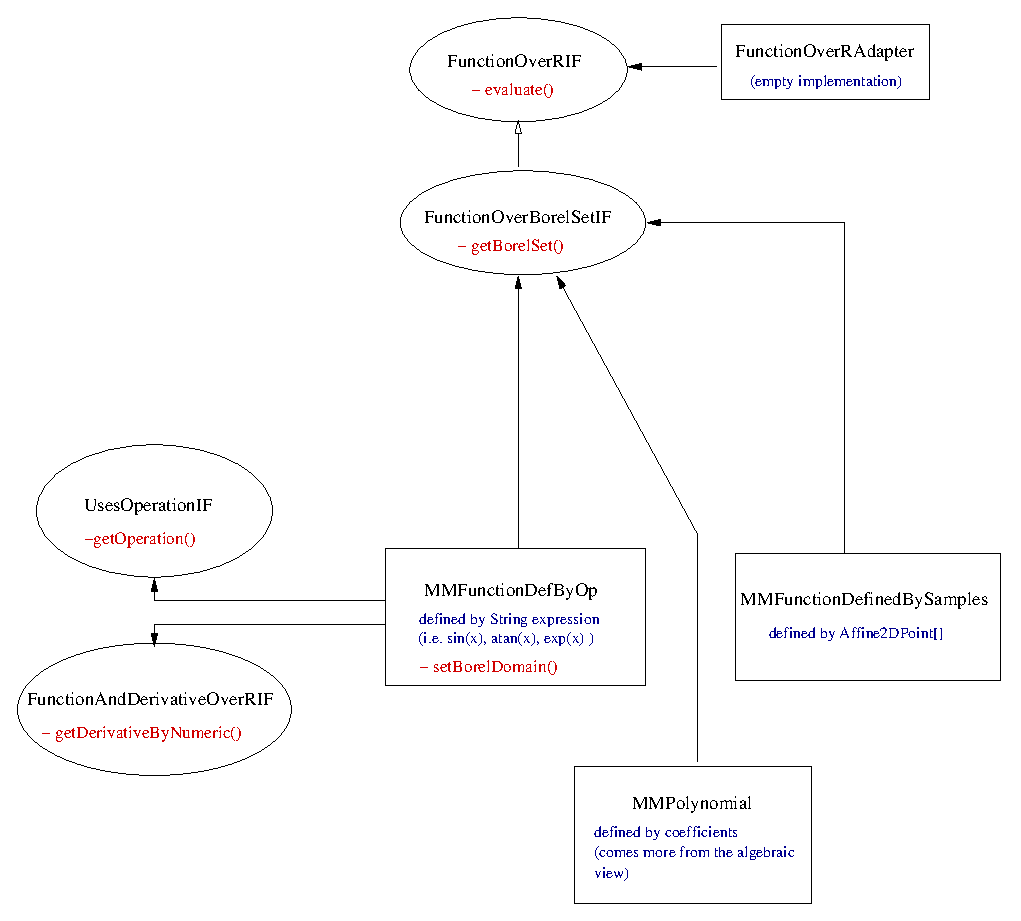
\includegraphics{images/FunctionStructureInMath}}

\section{Fig: Function Structure II}
\rotatebox{90}{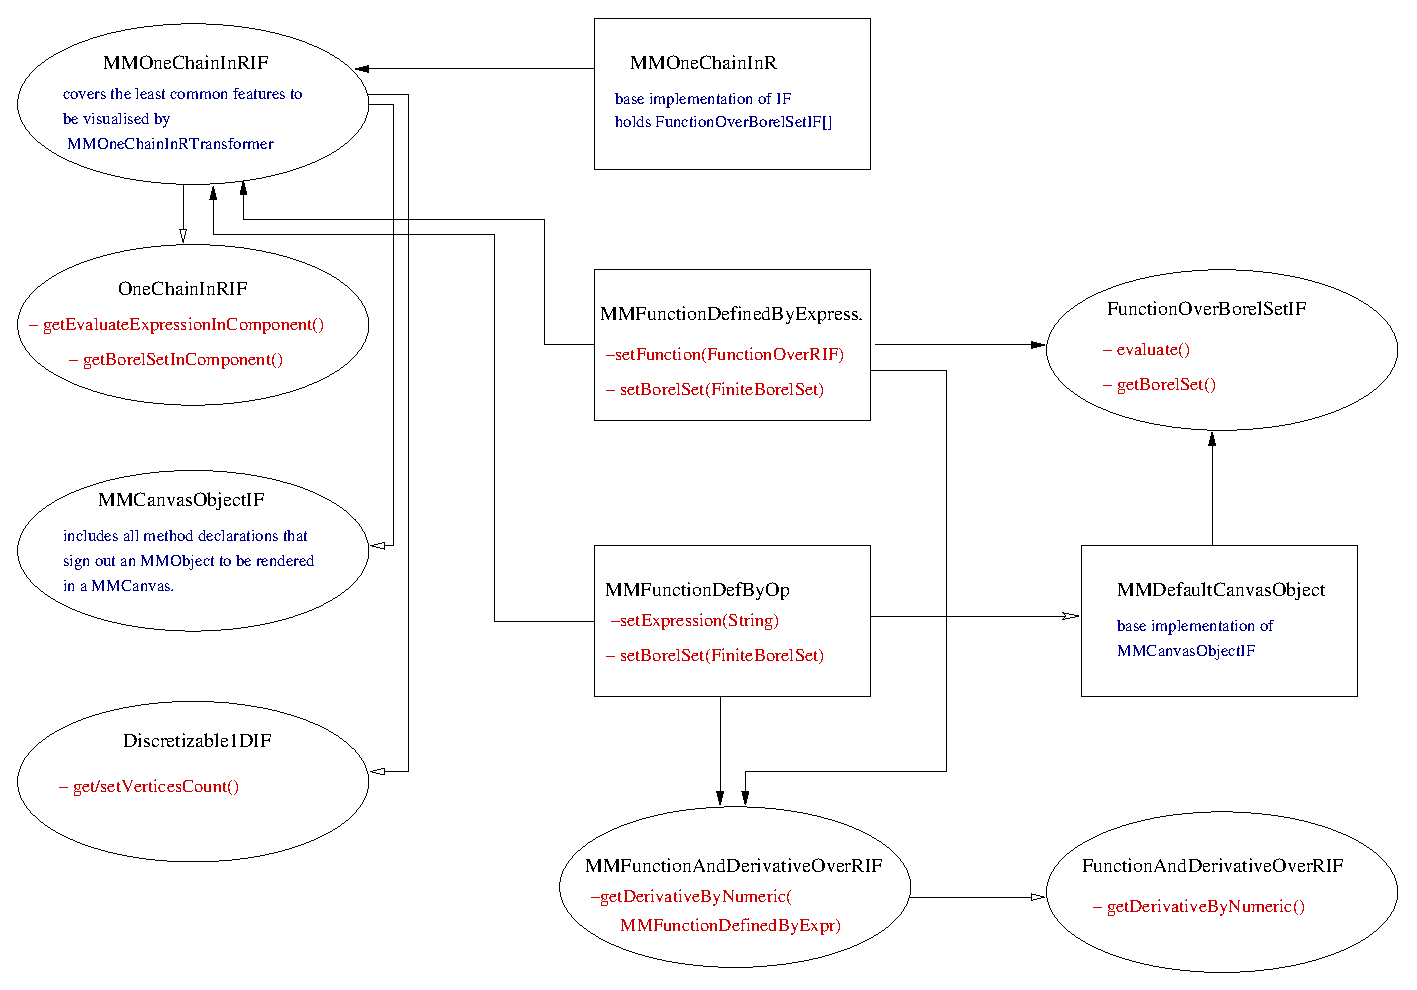
\includegraphics{images/MMFunctionStructure}}

\section{Fig: Implementation of Splines}
\rotatebox{90}{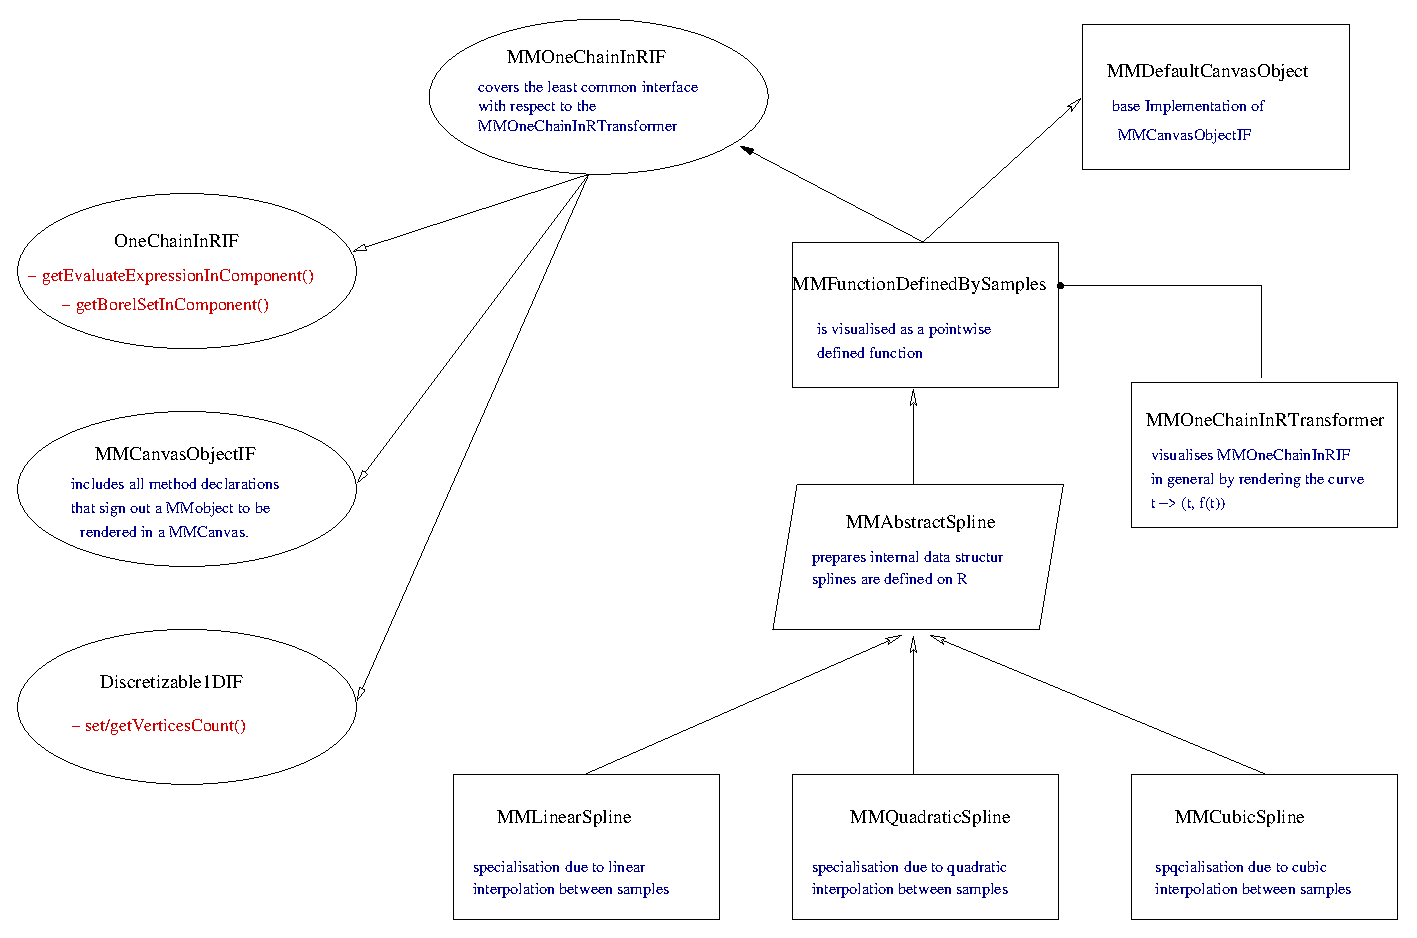
\includegraphics{images/MMSplineStructure}}

\clearpage
\chapter{The MathletFactory from a System Developer's Perspective}
\label{implementation_details}
This appendix contains an overview of the MathletFactory from a system developer's perspective. This perspective
is necessary for developing new MMObjects or display components that extend the set of mathematical entities represented by 
the MathletFactory.\\
In the following sections we omit the details, which can be found at the API documentation but give a structural overview that 
follows the Model-View-Controller architecture.
\section{MVC Architecture of the MathletFactory}
\subsection{Requirements}
Following the didactic model of Bruner, mathematics can be regarded as a system with three complementing representations: 
The {\it enactive} representation of a mathematical entity is determined by what you can {\it do} with it, the 
{\it iconic} representation is an image or sketch that {\it visualises} one or more of its properties and the 
{\it symbolic} representation {\it denotes} it in a formal language system. One of the main conclusions of Bruner's Theory 
is, that although professional mathematicians almost exclusively use symbolic representations, the other types of representations 
play a vital role in learning mathematics.\\
If we use this didactic principle as a requirement for the architecture of a mathematics learning framework, it makes 
sense to allow different representations for mathematical objects. This can be done best by using the 
Model-View-Controller Pattern\footnote{\cite{Bu96}}, an architectural pattern that separates the data of an entity from 
its presentation and application logic.

\subsection{Fundamental Concepts}
A good starting point when describing the MathletFactory is to describe what happens, when a student uses an applet
created with the MathletFactory.\\
If, for example, a student drags the graphical representation of a three dimensional vector on a canvas with the
mouse, the canvas generates an event that is sent to the {\tt CanvasController}. This instance checks all objects
contained in the canvas if they are meant, by using the mouse coordinates and the canvas' internal projection 
parameters. If an object has been picked and it can handle the type of event (by owning an appropriate handler), the 
event is delivered to it by calling {\tt MMObjectIF.doAction()}. The {\tt MMObject} then delegates the event to the 
specified handler, which processes the event (e.g.\ translating the end-point of the vector in a plane parallel to 
the viewport by transforming the new mouse coordinates to world coordinates) and modifies the state of the 
{\tt MMObject} (e.g.\ setting its coordinates to new values). After this it is checked, if any other objects depend 
on the vector (for example, the vector could be designated as normal for a plane). For this it is checked, if any 
{\tt Updater}s are associated to the object and if so, their {\tt update()} method is called, changing the state 
of any dependent objects (which in turn might also have other updaters and so on). After the update graph traversal 
has been finished, The views of the objects that were changed, are redrawn (both the graphical and the symbolic 
representation), by invoking {\tt render()} and {\tt draw()} in all transformers of the {\tt MMObject}. By this
the student is informed of the result of his action and may proceed with further actions.

\stepcounter{figcount}
\begin{center}
\resizebox*{16cm}{!}{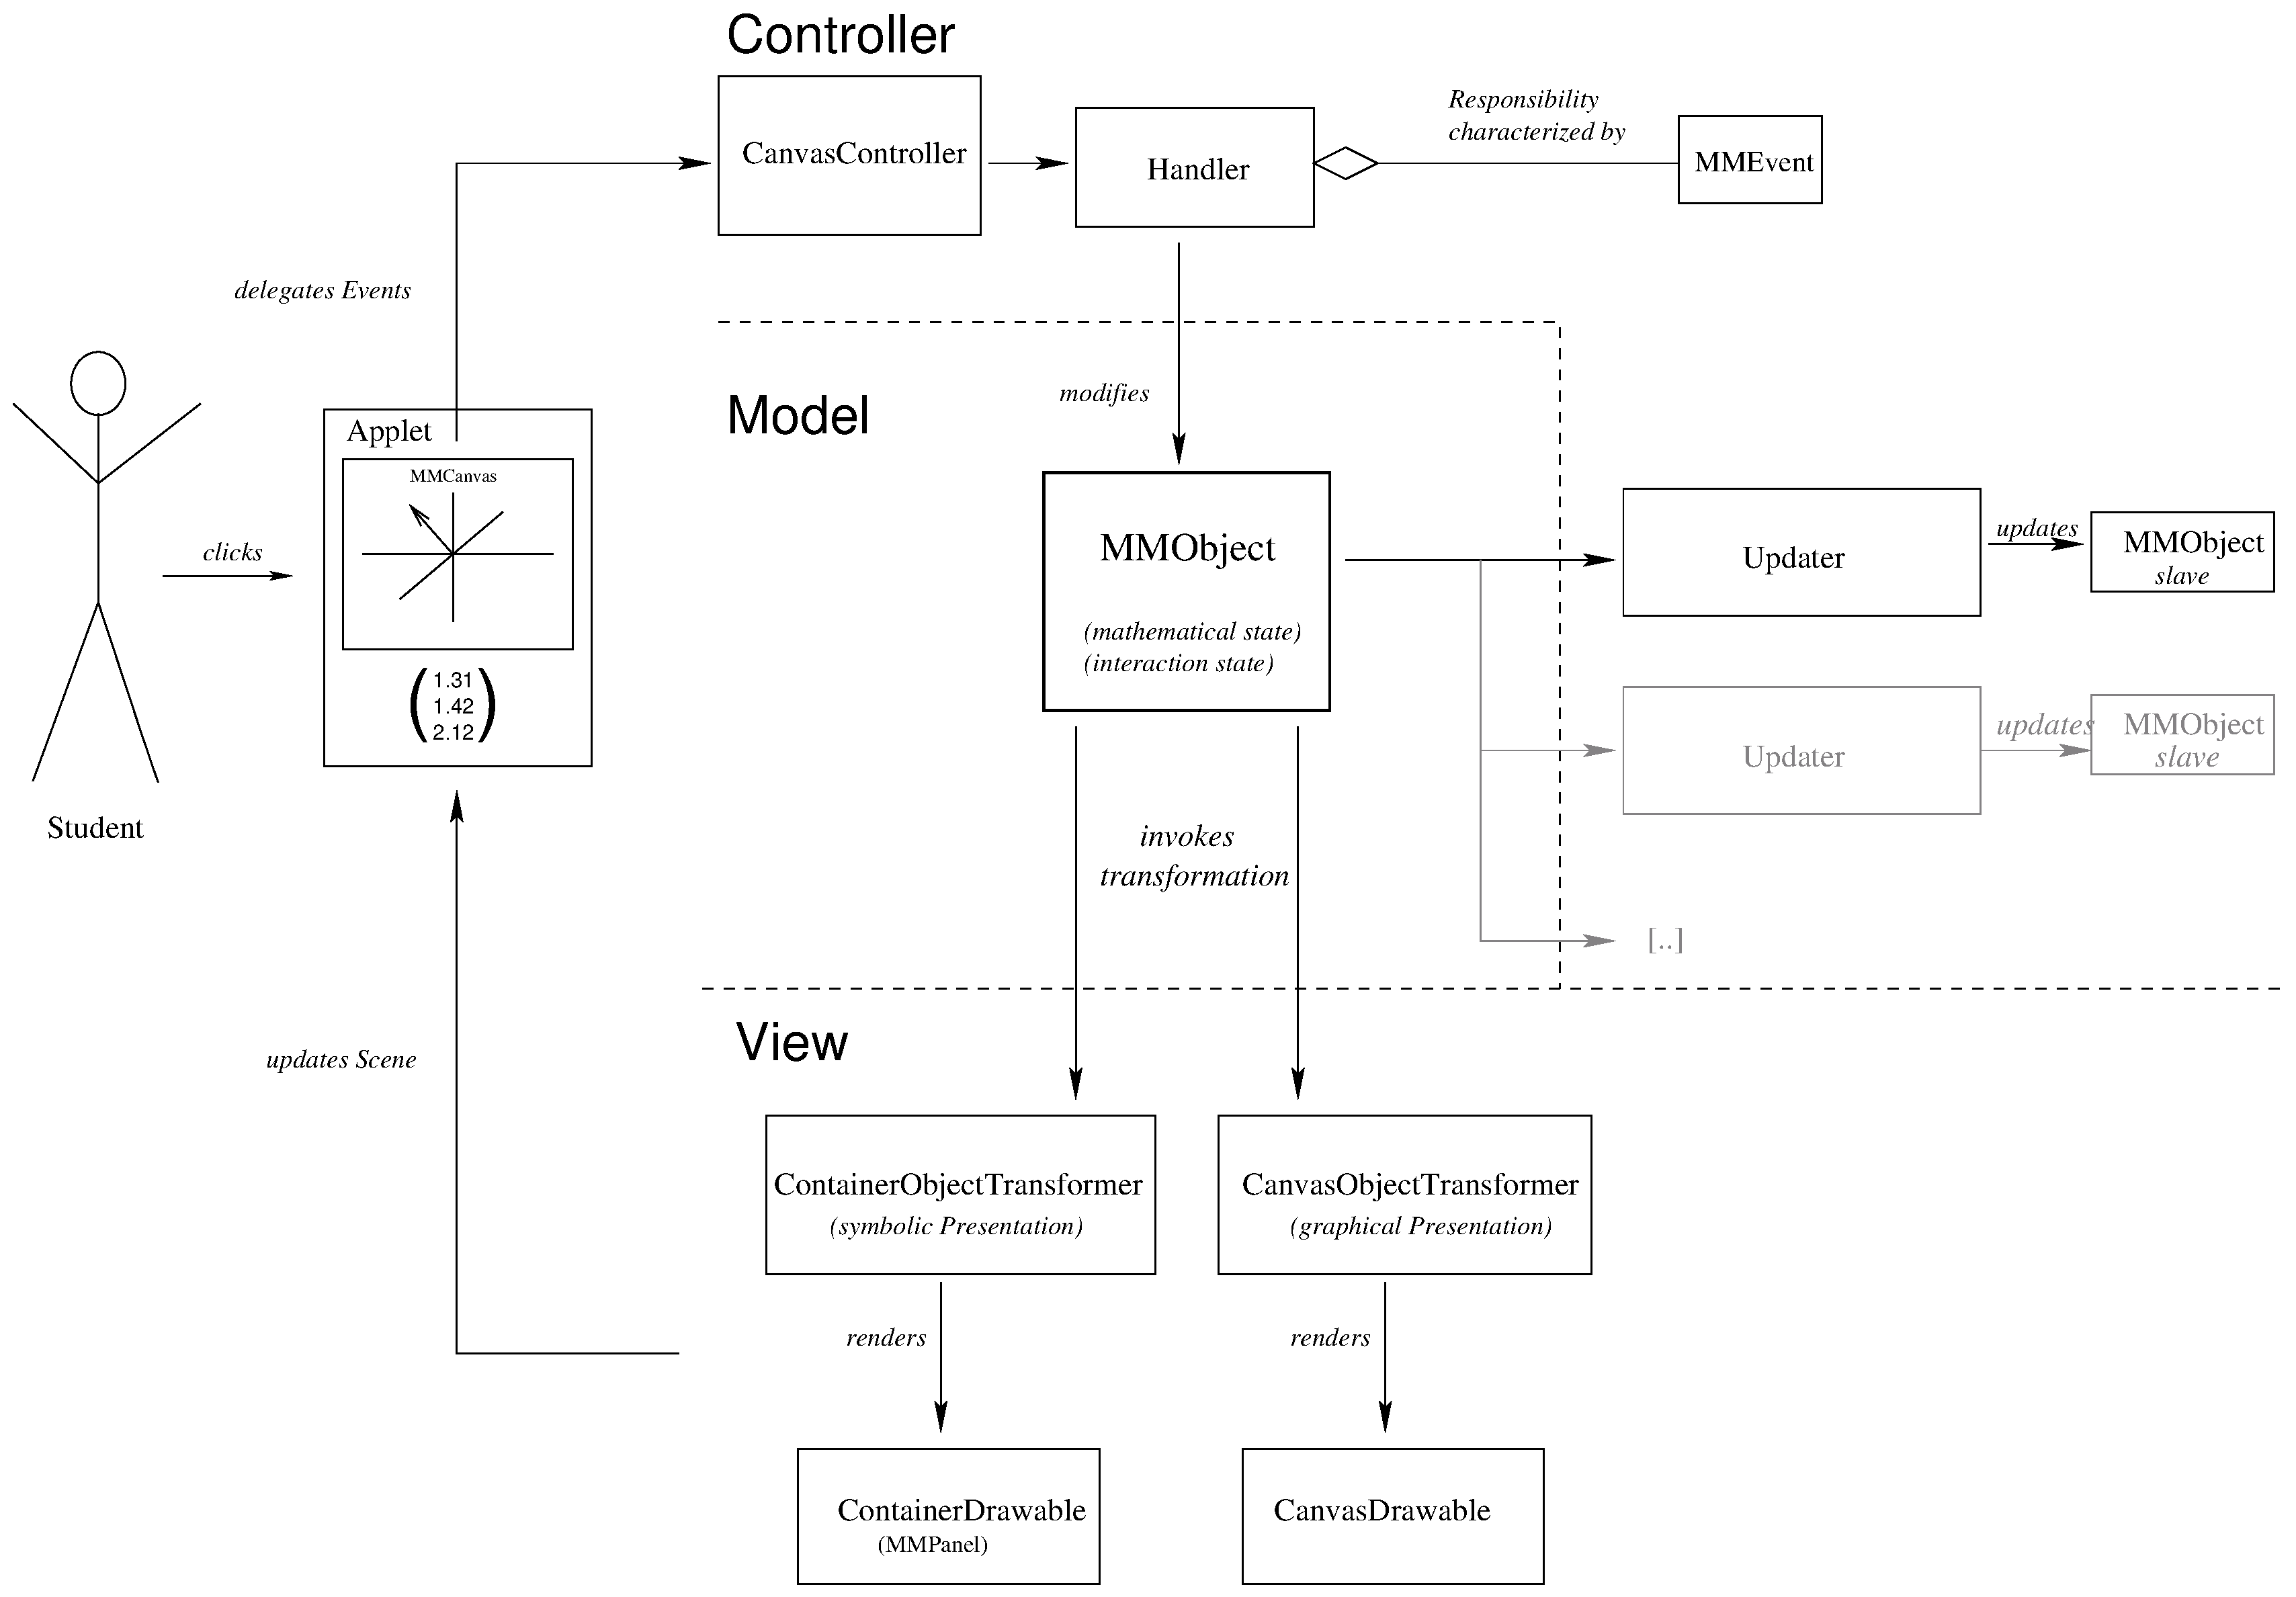
\includegraphics{diss_chapter/mvc}}\nopagebreak\\[1.0cm]\nopagebreak
\footnotesize{{\sf Fig.\ \arabic{figcount}: An action cycle in the MVC architecture }}\\[0.6cm]
\end{center}

\subsection{Model}
The core model used in the MathletFactory is the {\it MMObject}, represented
by a class that implements the {\tt MMObjectIF} interface. An instance of this class contains on the one hand the mathematical 
information of the object, on the other hand it also owns references to the handlers that allow its manipulation and to updaters
that connects the object with other MMObjects in the update graph. It also contains the link to the view components.

\subsection{View}
The view component consists basically of two objects: The {\it transformer} (represented by a subclass of {\tt GeneralTransformer})
the {\it drawable} (represented by the interface {\tt Drawable}). While the drawable is the actual displaying unit, the 
transformer establishes a link between model and drawable and knows how to repaint it, when the MMObject has changed.

\subsection{Controller}
In the controller section we differentiate between objects that directly manipulate MMObjects and those that are responsible
for constructing the update graph. The directly manipulating objects are represented by two different classes: Handlers (subclasses 
of {\tt MMHandler}) for manipulating iconic representations in a canvas (e.g.\ selecting and dragging vectors with the mouse) and 
panels (subclasses of {\tt MMPanel}) for editing symbolic representations. Note that the panel is also a drawable into which
the controller-code (which consists of only a few lines) has been integrated into.\\

\section{Arithmetic and Geometric Model}
In order to compute a wide variety of mathematical problems, the Mumie MathletFactory offers a flexible and economic model for
representing the geometric and arithmetic properties of mathematical entities and allows an accessible interface for easy 
manipulation. In the following, we briefly describe the model architecture of the basic entities. 

\subsection{Number Types}
Starting with the specification that all mathematical objects -- directly or indirectly -- use numbers, we assign to each MMObject a
specific number type that can be changed upon construction or sometimes even at run time. By this it is, for example, possible 
to use the same sequence object for displaying both real valued sequences and complex valued sequences. In the first case
the object is instantiated by invoking the constructor with the argument {\tt MComplex.class}, the second with the argument 
{\tt MDouble.class}. The implementation is done using an abstract base class {\tt MNumber} of which all number types
are subclasses. Currently, the following number types exist:\\

\stepcounter{figcount}
\begin{center}
\begin{tabular}{|p{5cm}|p{3cm}|p{5cm}|}
\hline
Number Type & Set of numbers modelled & Internal Java type used\\
\hline
{\tt MNatural} & $\mathbbm{N}$ & {\tt BigInteger}\\
\hline
{\tt MInteger} &  $\mathbbm{Z}$ & {\tt double}\\
\hline
{\tt MRational} &  $\mathbbm{Q}$ & {\tt long}\\
\hline
{\tt MBigRational} &  $\mathbbm{Q}$ & {\tt BigInteger}\\
\hline
{\tt MDouble} &  $\mathbbm{R}$ & {\tt double}\\
\hline
{\tt MComplex} &  $\mathbbm{C}$ & {\tt double}\\
\hline
{\tt MZmod5} & $\mathbbm{Z}/5\mathbbm{Z}$ & {\tt int}\\
\hline
\end{tabular}
\end{center}

The last is an experimental type that demonstrates the use of finite fields in the MathletFactory and will soon be replaced
by a generic class modelling $\mathbbm{Z}/p\mathbbm{Z}$.

\subsection{Vectors, Vector spaces and Matrices}
While the subclasses of {\tt MNumber} provide the base for one-dimensional number computing, the class {\tt NumberMatrix} --
representing an $m\times n$-matrix -- is fundamental for the calculation in linear spaces of higher dimension. As MMObjects 
it has also exclusively uses the generic number interface allowing each instance of a {\tt NumberMatrix} to represent a 
matrix of different number type.\\
The {\tt NumberMatrix} is extended by {\tt NumberTuple}, a class that represents  $m\times 1$-matrices and which is basically 
used as coordinates for vectors or matrix columns/rows. It therefore offers additional functionality like the norm, the dot 
product, etc.\\
Vectors in turn are modelled by subclasses of the abstract {\tt NumberVector}. It is a specific trait, that each vector
of the MathletFactory `knows' the vector space in which it exists and is represented by coordinates that are relative to its
associated basis. By this it is possible to transform all vectors of a chosen vector space by changing the space's basis.
The {\tt NumberVectorSpace} class therefore provides a wide range of methods to manipulate its basis. 

\subsection{Affine and Projective Geometry}
The vector space model is also used in the geometric classes. Like most CAG (Computer Aided Geometry) Modelling software.
All internal data is stored in homogeneous (i.e.\ projective geometry) coordinates. This allows the easy transformation
of mathematical entities also for affine geometry. For example, when calculating the intersection of two planes in the
three dimensional space $\mathbbm{R^3}$ (i.e.\ the intersection of 2D affine subspaces within a 3D affine space) simply
the projective hyperplanes have to be intersected, reducing the problem to finding the null space of the matrix that 
contains the projective coordinates of the subspaces' basis (see extended description of this example below).

\subsection{Numerical Computing}
Numerically, almost all affine and projective geometric operations -- like the example above -- base on the Gauss algorithm 
implemented in the class {\tt EchelonForm}. This ensures a high reusage and offers an easy optimisation opportunity: If the 
Gauss algorithm is made faster, a wide range of computations will be executed faster.

\subsection{Compound Example}
To demonstrate, how all the concepts described above work together, we give a `real life' example: In the mathlet depicted
below, the intersection of two planes in three dimensional is computed and displayed (For details refer to the documented 
source code):

\begin{center}
\resizebox*{8cm}{!}{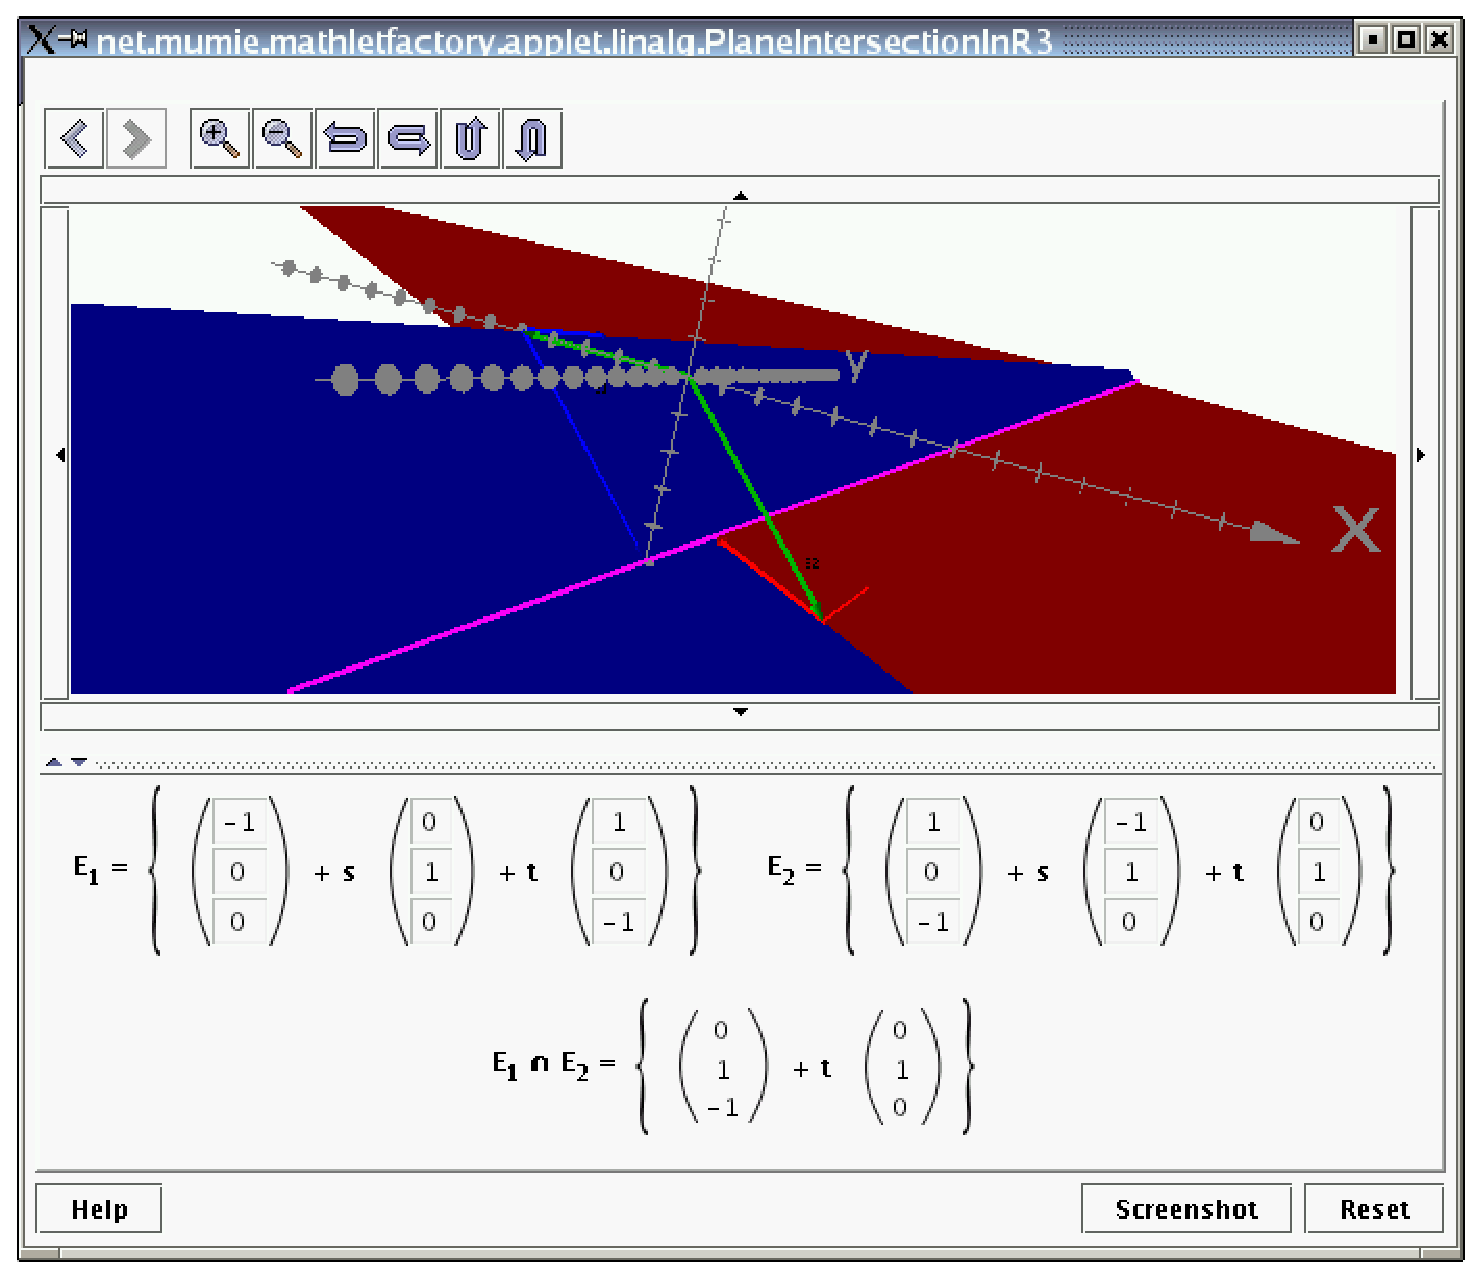
\includegraphics{diss_chapter/PlaneIntersectionInR3}} \hspace{0.5cm} \begin{minipage}[b]{8cm}
\begin{footnotesize}
\begin{verbatim}
	AffineSpace.intersected()
                 |
	AffineSpace.intersect()
                 |
	ProjectiveSpace.intersected()
                 |
	NumberVectorSpace.intersected()
                 |
	SolveHomogen.intersection()
                 |
	SolveHomogen.nullSpace()
                 |
	EchelonForm.getREFMatrix()
                 |
	EchelonForm.toReducedRowEchelonForm()

\end{verbatim}
\end{footnotesize}
\end{minipage}\nopagebreak\\[0.5cm]\nopagebreak
\footnotesize{\sf Fig.\ \arabic{figcount}: The intersection of two planes in three-dimensional space and its stack trace to the Gauss algorithm}\\[0.3cm]
\end{center}

This starts in by invoking the method {\tt AffineSpace.intersected(AffineSpace with)} in one of the planes
with the other as argument (the plane class descends from the affine space class). This method does nothing but the
invocation of its projective representation to intersect with the projective representation of the other plane.
This is done by giving their two vector bases to the method {\tt SolveHomogen.intersection(NumberTuple[] span1, NumberTuple[] span2)}
which in turn calls the {\tt nullSpace(NumberMatrix matrix)} method with a (3$\times$6) matrix as argument that contains all the 
base vectors as columns. This method in turn uses the Gauss algorithm implemented in {\tt EchelonForm.getREFMatrix(NumberMatrix matrix)}
to transform the matrix to reduced echelon form to determine its null space basis. The null space basis is then used as parameters 
for constructing the basis of the intersecting space, which is returned by the {\tt intersected()} method.

\chapter{Algebraic Object Model and Formal Languages}
Since often it is not only needed to let the application developer perform computations with the MathletFactory but also the 
student (or teacher/tutor) himself, the arithmetic and geometric model is complemented by an algebraic model that allows the 
input of expressions in a formal language. By this, the flexibility of the mathlets is increased and allows them to be used
as tools in open learning scenarios.

\subsection{Lexical, Syntactic and Semantic Analysis}
In order to analyse and interpret a formal language, we need structures that operate on three different levels of language: the first 
is the lexical analysis which analyses the alphabet of symbols being used, the second is the syntactic analysis that applies
the rules for building words and sentences. On the third level we have the semantic analysis that analyses the meaning of the
words.\\

\stepcounter{figcount}
\begin{center}
\resizebox*{15cm}{!}{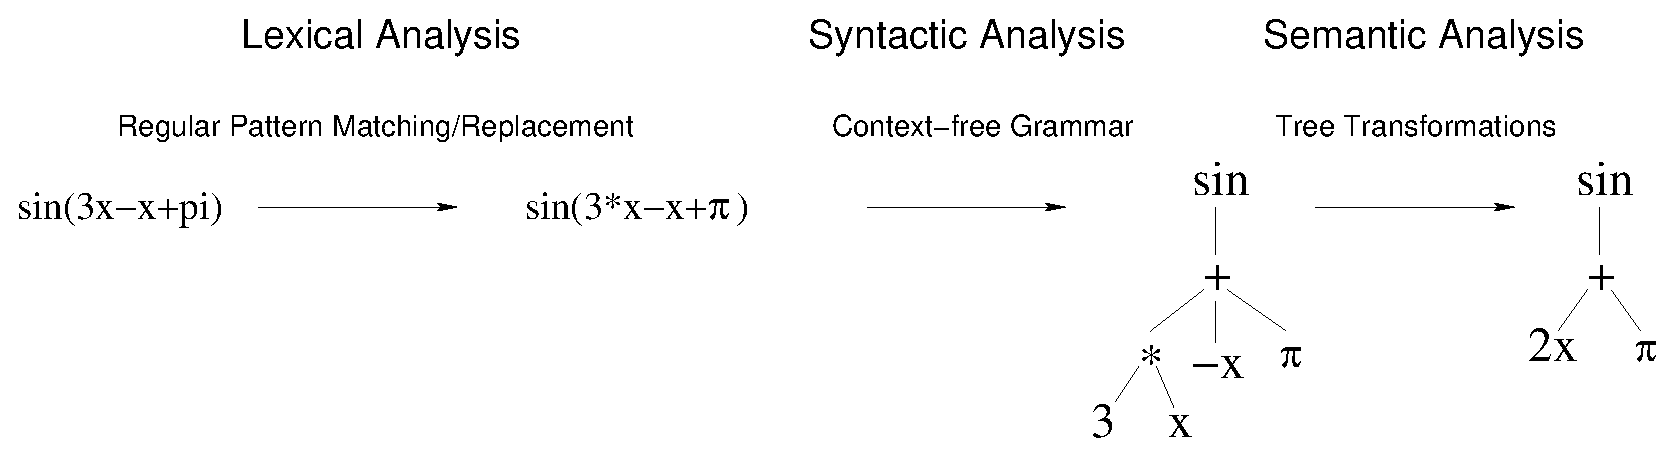
\includegraphics{diss_chapter/languageProcessing}}\nopagebreak\\[0.5cm]\nopagebreak
\footnotesize{\sf Fig.\ \arabic{figcount}: The different stages in mathematical
  expressions analysis performed by the MathletFactory}\\[0.6cm]
\end{center}

In the MathletFactory, each stage of language processing is performed by a specific unit: The lexical analysis is performed by 
a set of regular expressions (which also do some replacements that allow an increased robustness like {\tt 2x} $\rightarrow$ 
{\tt 2*x}) and a small scanner unit. The syntactic analysis is done by a parser that implements a context-free grammar (see below) 
and the semantic analysis is left to a rule-based tree automaton that operates on the operation tree generated by the parser.\\
Note that it is quite easy to reproduce a string out of the tree representation by doing a depth-first 
order traversal, thus closing the sequence to a loop. This is very important for interactive work with mathematics, where the user 
enters an expression, watches the response of the system and may want to re-edit his input for a receiving a different result.

\subsection{Introduction to Formal Languages}
The main idea of the MathletFactory's algebraic object model takes advantage of the formal languages used in mathematics. 
Computer science has developed a rich set of methods to interpret these formal languages of which we can only give a 
short introduction, see \cite{HU79} for details.\\
A formal language can be defined as a concatenation of symbols from an alphabet. These concatenations are called the 
{\it words}. The formal language ${\cal L}(\Sigma)$ over an alphabet $\Sigma$ that consists of all possible words can thus inductively
be defined as:

\begin{enumerate}
\item $\sigma \in {\cal L}$ for all $\sigma \in \Sigma$.
\item $w \in {\cal L}$ for $w = u.\sigma$ with $u \in {\cal L}, \sigma \in \Sigma$.
\end{enumerate}

with $.$ being the concatenation operator. The language that consists of all words over $\Sigma$ is also called 
$\Sigma^*$, where the $^*$-operator means, that the resulting set contains all finite concatenations 
$\sigma_1.\sigma_2\ldots\sigma_n, n \in \mathbbm{N}$ of symbols $\sigma_i \in \Sigma$, and the empty 
word $\varepsilon$.\\

Of course we are more interested in languages that allow only certain words. For example, we may want {\tt (x+1)} to be a 
word of our language, but not {\tt +)1)x}. We thus need a higher structure that tells us, which words belong to the language, a 
{\it grammar}.\\ 
A grammar is defined by the accepted alphabet (the {\it terminals}) and by a set of explicit rules how a word can be decomposed 
into these. For example, one could state the following rules for simple arithmetic expressions of numbers represented by
{\tt NUM}:\\ 
\renewcommand{\thefootnote}{\fnsymbol{footnote}}

\begin{enumerate}
\item {\tt +}, {\tt -}, {\tt *}, {\tt /} $\in {\cal L}$,  {\tt NUM} $\subset {\cal L}$,\footnote{Note, that for avoiding trivial rules 
it is better to regard a number like {\tt 1234} to be represented by a single symbol, not as a concatenation of symbols as one would 
presume by the fact that it is a concatenation of digits in our common writing system. In the following we will also regard function 
identifier like {\tt cos} as a single symbol in order to keep our grammar compact.}
\item $w \in {\cal L}$ for $w = u.${\tt *}$.v$ or $w = u.${\tt /}$.v$ with $u,v \in {\cal L}$,
\item $w \in {\cal L}$ for $w = u.${\tt +}$.v$ or $w = u.${\tt +}$.v$ with $u,v \in {\cal L}$.
\end{enumerate}
\renewcommand{\thefootnote}{\arabic{footnote}}
\addtocounter{footnote}{-1}

We have already differentiated between products and sums of rational numbers, because for the semantic analysis
(i.e.\ evaluating the arithmetic expressions) it is necessary to consider the precedence of operations.
One could define grammars like we did in the example above, but for handling more complex grammars it is useful to
state a grammar in the Backus-Naur form (BNF), which regards grammars as a tuple $(T,N,s,R)$, where $T=\Sigma$
is the set of terminals, $N$ is the set of nonterminal symbols (i.e.\ variables that may contain concatenations of terminals), $s$ 
is the name of the starting variable (i.e.\ the variable whose content is tested to be a valid word of the specified 
language) and $R \subset (N \cup T)^*.N.(N \cup T)^* \times (N \cup T)^*$ is the set of rules that need to apply for a 
word of the specified language:

\begin{footnotesize}
\begin{verbatim}
G(T,N,s,R)

 T:     NUM,'+','-','*','/'
 N:     expr, term, fac
 s:     expr
 R:     
 (1)    expr      ->      term { '+' term } | term { '-' term } .
 (2)    term      ->      fact { '*' fact } | fact { '/' fact } .
 (3)    fact      ->      NUM.
\end{verbatim}
\end{footnotesize}

We see, that the operator precedence is ensured by using different variables for summands and for factors. The 
expression {\tt 3*4+1} could thus be tested by the grammar as follows (we enclose the symbol with its type in 
parentheses):\\

\begin{tabular}{ll}
{\tt (expr 3*4+1)} & $\stackrel{(1)}{\rightarrow}$ {\tt (term 3*4).+.(term 1)}\\
& $\stackrel{(2)}{\rightarrow}$ {\tt (fact 3).*.(fact 4).+.(fact 1)}\\
& $\stackrel{(3)}{\rightarrow}$ {\tt (NUM 3).*.(NUM 4).+.(NUM 1)}.\\
\end{tabular}\\

After this none of the rules can be applied to the expression anymore which means that {\tt 3*4+1} is a word specified
by $G$. This testing method also gives an idea, how a parser that accepts words of ${\cal L}(G)$ could be 
implemented: By a recursive reduction algorithm, where each rule is modelled by an according method.\footnote{This is 
called the Top-Down approach, which is mainly used in functional or rule-based language implementations, 
imperative language implementations often also use a Bottom-Up approach, where for each step only as much symbols are 
read in as needed for applying the next rule.}\\

\subsection{Types of Grammars}
\label{types_of_grammars}
Noam Chomsky has provided a hierarchy of grammars where each type produces a language that is a subset of a language 
produced by a lower type. The type of a grammar depends completely on the specified rules $R$:\\
\begin{center}
\begin{tabular}{l|l|l}
Type & Name & Constraints for $R$\\
\hline
1 & context sensitive & $|u| \leq |v|$ for all $R: u \mapsto_G v$\\
2 & context free & $R \subseteq N \times (N \cup T)^*$\\
3 & regular &  $R \subseteq N \times (\{\varepsilon\} \cup T \cup N.V)^*$
\end{tabular}\\
\end{center}
This means for example, that regular grammars produce only a subset of context free grammars, which in turn produce
a subset of context sensitive languages. Which type suits our needs? There are some features for which we need
at least a context free grammar. For example, an expression containing parentheses is only valid in mathematics, when
every opening parenthesis has its closing counterpart. On the other hand we want to use parentheses on all levels.
This means we need a rule $r \in R$ that has the form {\tt prim} $\rightarrow$ {\tt '(' expr ')'}, which is not
possible for regular grammars, which allow no terminals on both sides of a non-terminal. Context sensitive grammars
in turn would allow rules with non-terminals and terminals mixed on the left side thus allowing a higher semantic 
analysis already in the syntax phase, one could, for example, add something like with the following rule:\\
{\tt  NUM '*' '(' VAR '+' VAR ')'} $\rightarrow$ {\tt '(' NUM '*' VAR '+' NUM '*' VAR ')'},\\
thus implementing the distributive law for words containing two variables {\tt VAR} multiplied with a number {\tt NUM}. 
But as the reader might guess, a program that parses context sensitive languages is hard to implement, 
so we do things like this in a separate semantic analysis step (see \ref{transformations}).\\

\subsection{From Syntactic to Semantic Analysis}
After the parser has accepted the mathematical expression, we need to transform it into a data structure that allows
easy semantic analysis. In our case it is suitable to represent it as a syntax tree or as a word of a regular tree 
language \cite{Co03}. For example, sin(2x+$\pi$) is interpreted as {\tt (sin (+ (* 2 x) pi))}.
The expression can then be symbolically transformed by using tree automata (see below) or numerically evaluated, which is 
done by a recursive procedure that evaluates the tree from the leaves (numbers or variables and parameters with 
assigned values) up to the root node.


\subsection{Formal Languages Used by the MathletFactory}
The MathletFactory uses two formal languages, which are both context free and read by a recursive descent parser \cite{ASU86}: 
The operation language {\it Op} and the relation language {\it Rel}.
\paragraph{The Operation Language {\it Op}}
The language {\it Op} is used for modelling algebraic operations as they occur in functions, equations, etc. It can be 
used by any mathematical object that can be characterised by a numerically evaluable symbolic expression.
The grammar of {\it Op} is as follows:\\

\begin{scriptsize}
\begin{verbatim}
G(T,N,s,R)

 T:      NUM, VAR, SIN, COS, SINH, COSH, EXP, ASIN, ACOS, LN, SQRT, '+', '-', '*', '/', '^',
 N:      expr, term, fac, pot, prim
 s:      expr
 R:
 (1) expr      ->      term { '+' term } | term { '-' term } .
 (2) term      ->      fact { '*' fact } | fact { '/' fact } .
 (3) fact      ->      SIN pot | COS pot | SINH pot | COSH pot | EXP pot | LN pot | ABS pot 
                       | ASIN pot | ACOS pot | TAN pot | ATAN pot | SQRT pot | FLOOR pot | pot.
 (4) pot       ->      prim {'^' prim}.
 (5) prim      ->      VAR | NUM | '(' expr ')' | '|' expr '|' .
\end{verbatim}
\end{scriptsize}

\paragraph{The Relation Language {\it Rel}}
\label{rel_grammar}
The language {\it Rel} is used for modelling algebraic relations as they occur in set definitions, propositions, etc.
As one might already guess from the fact that relations consist of operations, words of {\it Op} are part of the letters 
of {\it Rel}. More precisely, the {\it Rel} terminal {\tt SIMP} is a simple relation that contains a left and right 
hand side {\tt expr$_{i}$} $\in$ {\it Op}, which are separated by a relation sign ($=$,$\neq$,$\ge$,$\le$,$>$ or $<$).
The grammar of {\it Rel} is as follows:\\

\begin{scriptsize}
\begin{verbatim}
G(T,N,s,R)

 T:      SIMP, NOT, AND, OR, NOT
 N:      rel, cla, sub, prim 
 s:      rel
 R:
 (1) rel       ->      sub { OR sub }.
 (2) sub       ->      cla { AND cla }.
 (3) cla       ->      NOT prim | prim.
 (4) prim      ->      SIMP | ALL | NULL | '[' rel ']'.
\end{verbatim}
\end{scriptsize}
Note that in {\it Rel} we use square brackets for overriding precedence, whereas in {\it Op} we use parentheses, 
allowing to parse a complete relation containing operations in a single pass.

\subsection{Tree Architecture}
After the syntactic analysis (i.e.\ the construction of the operation/relation tree from a user/application provided string), 
the semantic analysis (i.e.\ transformation or evaluation of the tree) takes place, again initiated by user or application
action. We demonstrate this in a short example:


\stepcounter{figcount}
\begin{center}
\resizebox*{3cm}{!}{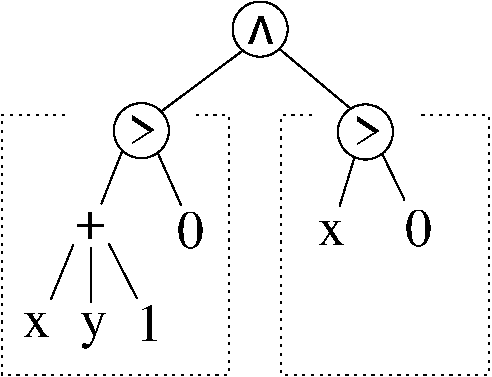
\includegraphics{diss_chapter/relation}}\\[0.2cm]\nopagebreak
\footnotesize{\sf Fig.\ \arabic{figcount}}\\
\end{center}

In the figure above the relation $x + y +1 > 0 \wedge x > 0$ is displayed in its tree represen\-tation (e.g.\ as a parsed 
result of the string `{\tt x+y+1>0 AND x>0}'). This tree has two levels: a relation level (the encircled nodes) and an 
operation level (the nodes below the relation nodes). The relation consists of $\wedge$-Conjunction as root node with two 
{\it simple} relations ($x+y+1 > 0$ and $x > 0$, the dashed boxes in the figure) as leaves. The relation leaves contain 
the operations $x + y + 1$, $0$ and $x$, $0$. After binding $x$ and $y$ to certain numeric values, the relation can be 
evaluated, returning either {\tt true} or {\tt false}, depending on the evaluation results of the operations.\\

The approach of using tree representations for mathematical expressions is adopted by all modern Computer Algebra Systems 
(e.g.\ \cite{Wo91}, \cite{Wa91}, \cite{Mo93}), but their almost purely functional 
model allows neither typing (e.g.\ no type distinction between operations and relations)\footnote{For example, in Maple variables 
can hold relations as well as boolean or numerical values, making expressions like {\tt y = (y=1);} or 
{\tt plot(sin(true),x=0..Pi);} computable.} nor the integration in an object oriented graphical user interface.\\ 
For our requirements, we will adopt the concept of a functional representation, but merge it with an object oriented model.
This means for the architectural design that we use the different types {\tt Operation} (any symbolic expression that can 
be numerically evaluated) and {\tt Relation} (any symbolic expression that can be either true or false). We choose these 
entities because they are closed under the most transformations we will apply onto them (for example, opposed to the set
of equations -- the set of relations is closed under equivalence transformations, the set of analytic operations is closed 
under derivation), so we can still use a functional model  when transforming trees of each type.

\paragraph{Tree Representation vs. Flat Representation}
Apart from being a construct of formal languages over which human-computer interaction is possible, a tree architecture also 
grants a greater flexibility than flat structures. For example, if we want to model a finite representation of a Borel 
$\sigma$-algebra in $\mathbbm{R}$ this could be implemented by a single class, owning a list of intervals, upon which 
the operations {\tt intersect}, {\tt join}, {\tt complement} etc. are resolved. This can be quite costly if we want to 
compute the join or intersection of two Borel sets that are widely `scattered', though the user will usually test inclusion 
in the result only for some points or a single interval displayed on the screen. Also, we could not model the special case of 
infinite intervals like $\mathbbm{Z}$, $\mathbbm{R}\backslash2\pi\mathbbm{Z}$, etc. which we need when displaying periodic 
behaviours.\\
The solution to this problem is to implement the Borel set as a tree structure that has intervals and 
`periodic intervals' as leaves and operations upon Borel sets as inner nodes. When the user wants the set to be displayed
on the screen, the observed interval and an $\varepsilon$ for precision (e.g.\ pixel width) is given to the Borel set and 
a distribution of points and lines satisfying these parameters is computed.\\
As this example suggests, constructing trees of mathematical entities allows a higher degree of generalisation 
without losing flexibility and simplicity. We will also see in section \ref{model_application} that trees are easily 
transformable, adding a lot of functionality to tree-structured mathematical entities.


\subsection{Basic Tree Model}
All tree-organised implementations of mathematical entities share a common base class, the {\tt AbstractTreeNode}, which
offers abstract tree functionality regardless of type, like adding or removing children, searching and replacement of 
descendants, etc. From these, the basic nodes for mathematical entities are derived (at this time {\tt OpNode}, 
{\tt RelNode} and {\tt SetNode}), the subclasses of which are the concrete implementations of mathematical operations 
and operands. The tree of these nodes is referenced by the model of the mathematical entity ({\tt Operation}, {\tt Relation}, 
{\tt BorelSet}), which serves as static container and fixed reference when performing tree transformations:\\

\stepcounter{figcount}
\begin{center}
\resizebox*{14cm}{!}{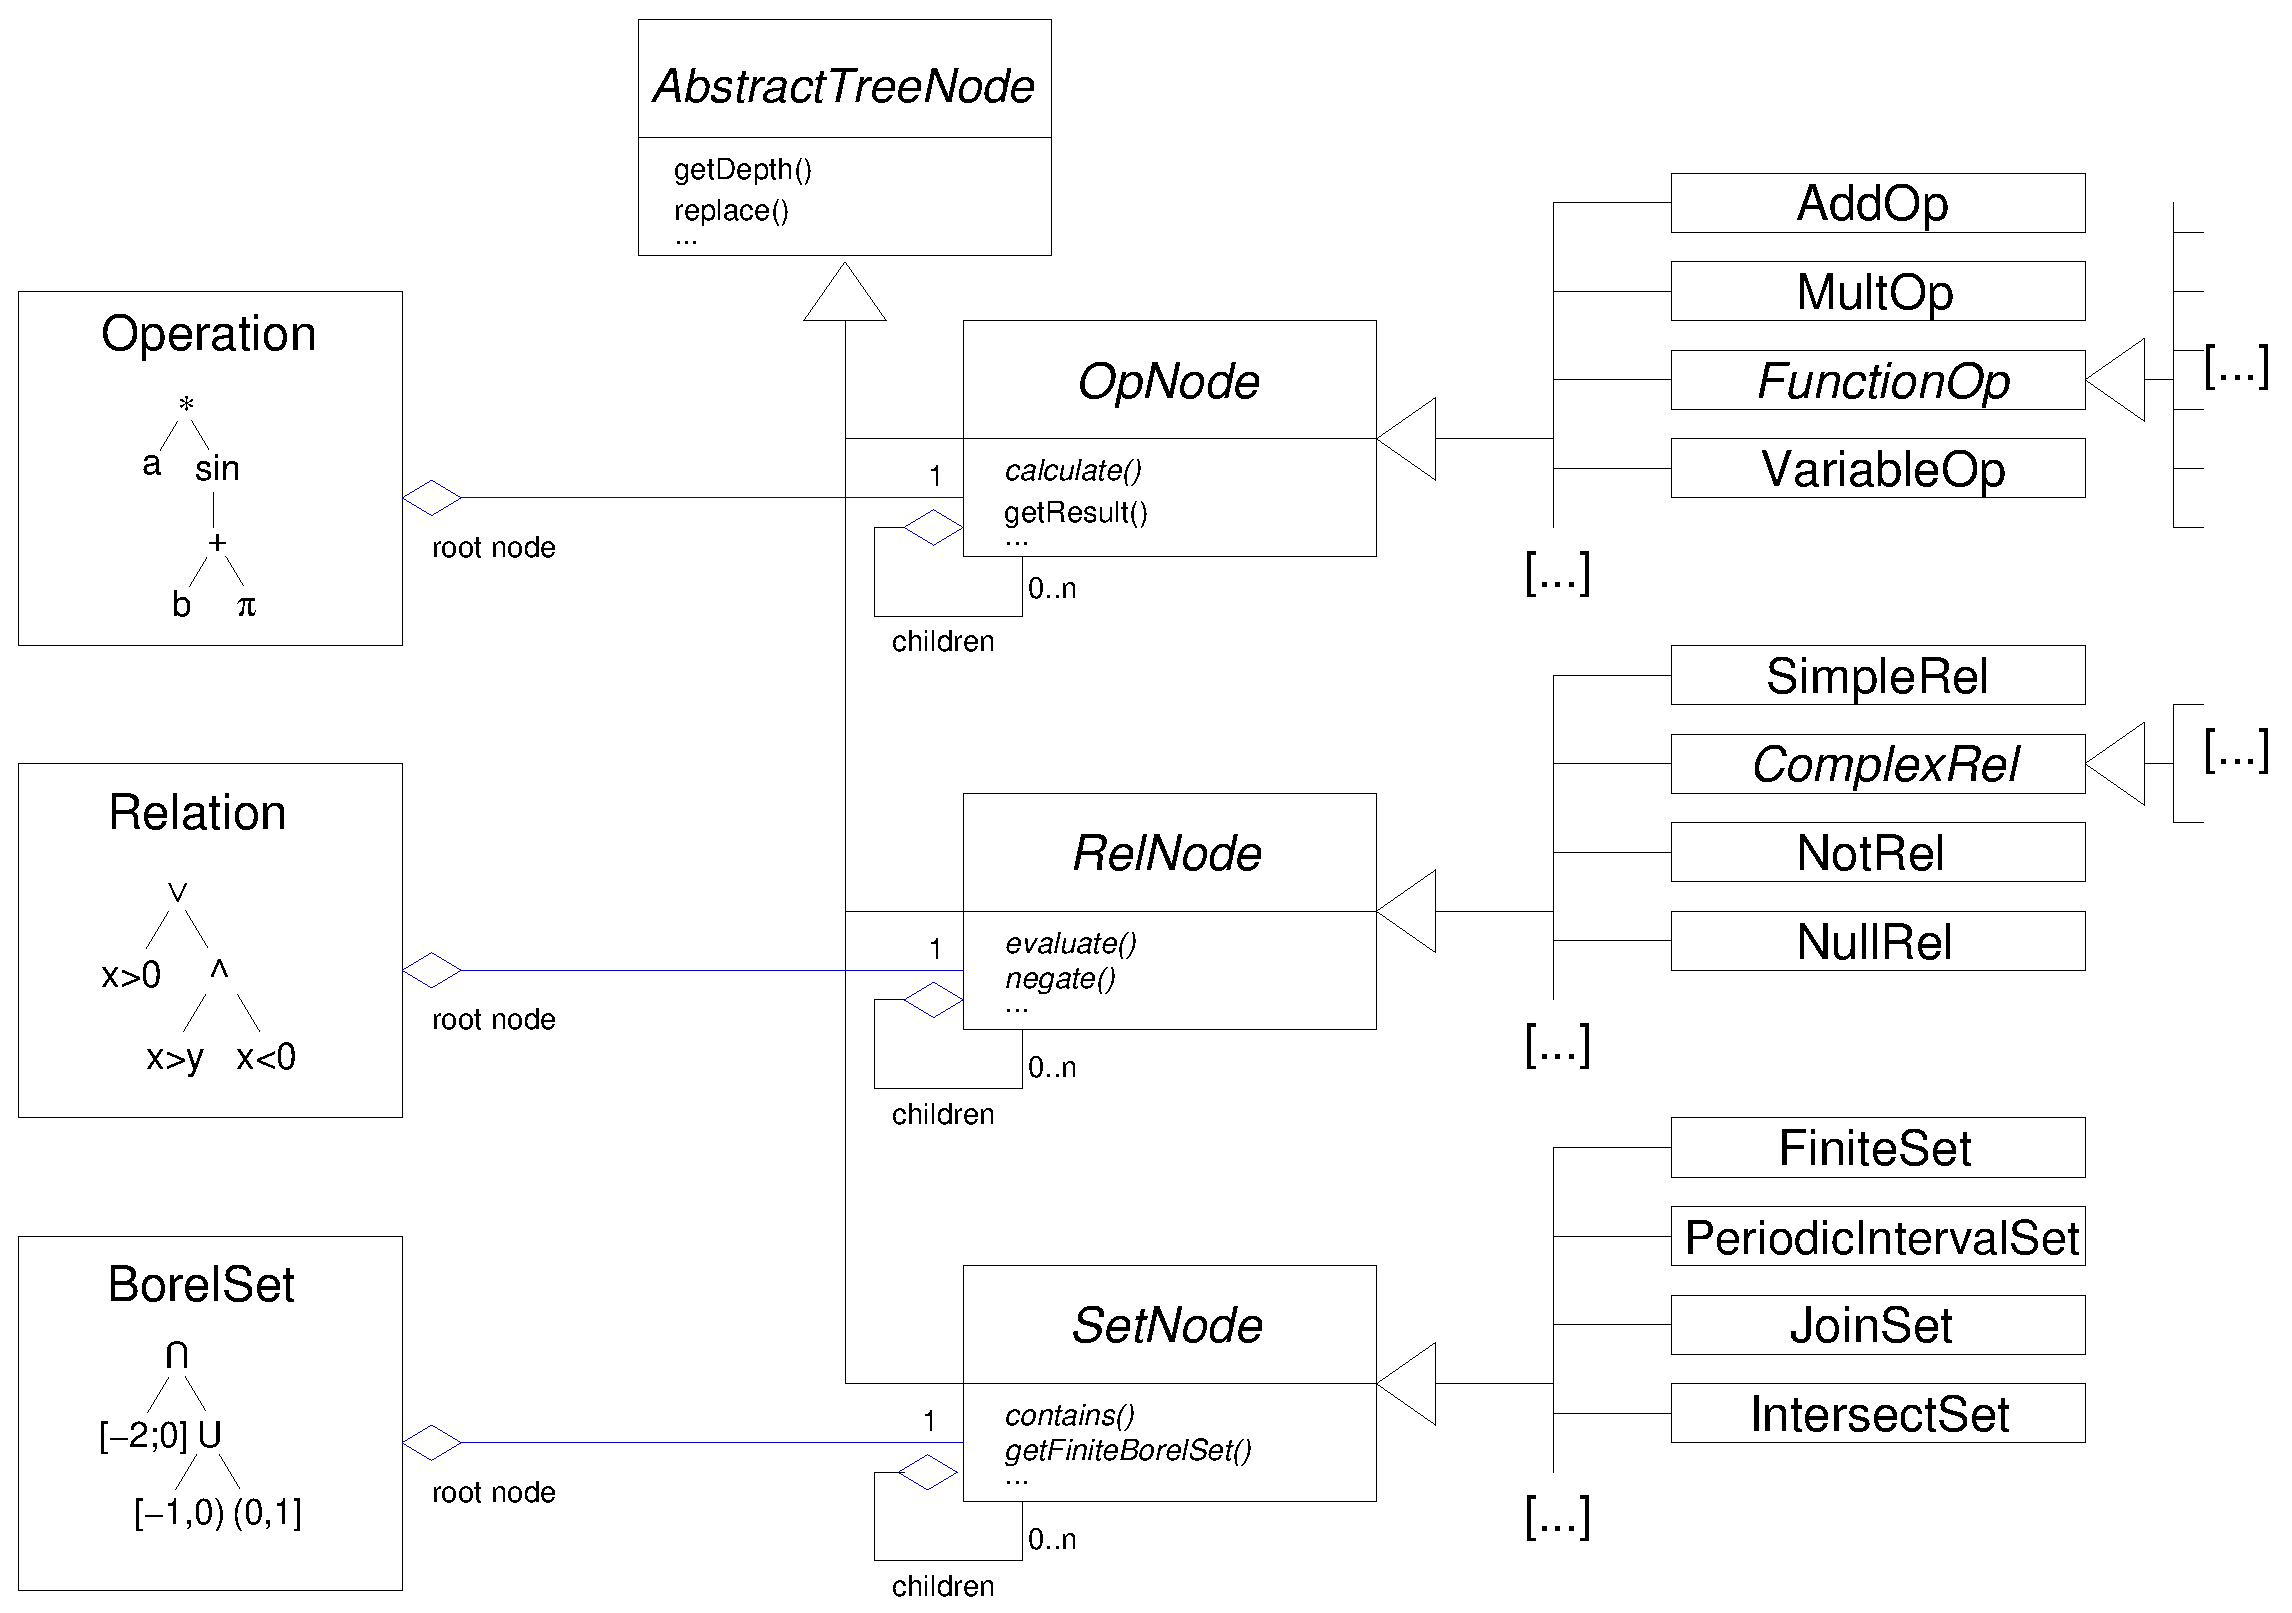
\includegraphics{diss_chapter/treeNodes}}\nopagebreak\\[0.5cm]\nopagebreak
\footnotesize{{\sf Fig.\ \arabic{figcount}: Inheritance and aggregation model of tree nodes}}\\[0.6cm]
\end{center}

\subsection{Object Model of Operations}
\paragraph{Generation and Structure of Operations}
The Language {\it Op} is syntactically analysed by an recursive descent parser. When parsing an expression it creates a 
corresponding operation tree that is contained in an {\tt Operation} object. The operation tree consists of nodes that 
are of type {\tt OpNode} and whose inner nodes are functions and operations while the leaves are basically variables and 
numbers. For example, parsing the expression "sin(2x+$\pi$)" generates the operation tree {\tt (sin (+ (* 2 x) pi)}:\\

\stepcounter{figcount}
\begin{center}
\resizebox*{6cm}{!}{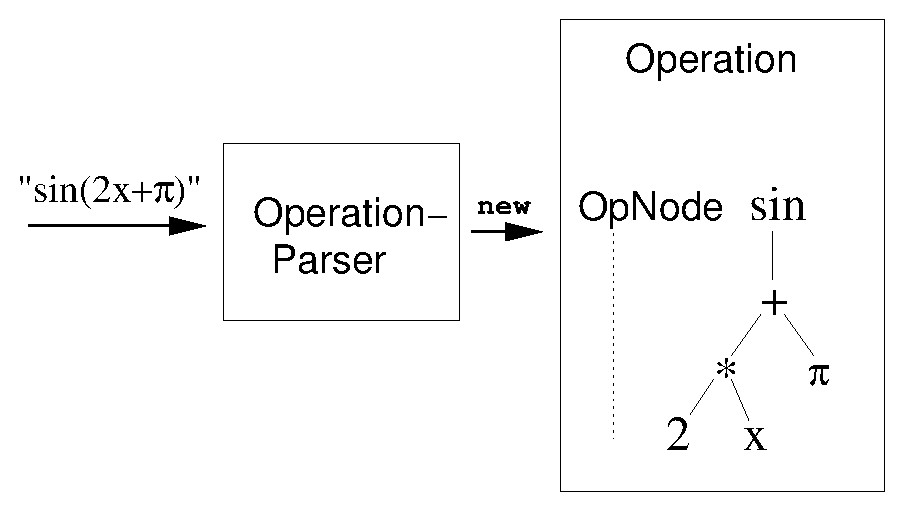
\includegraphics{diss_chapter/op_Parser}}\\[0.2cm]\nopagebreak
\footnotesize{\sf Fig.\ \arabic{figcount}}
\end{center}

The {\tt Operation} class bundles the functionality for any operation that can be found in a function or on the left or 
right hand side of an equation, etc. It contains a reference to the operation tree and keeps track of state information 
like the variables used and normalisation status (see below).\\
The operation tree is made of instances of the class {\tt OpNode}, which is an abstract class that provides the common 
functionality for all operation nodes. It models an elementary operation with a factor and an exponent so the above 
example could also have the form {\tt (sin (+ 2x pi))}. From the functional view the factor and the exponent are not 
essentially necessary, since there are also nodes for power and multiplication operations, but with addition and 
multiplication being the most common operations, this reduces the depth of most trees. This again decreases the costs 
of analysis and synthesis of larger trees and allows a higher amount of order within the trees (for example, children 
of a multiplication node can be ordered by power, making fraction handling easier). 
Adding factor and exponent fields to an operation node is also a common technique used in CAS \cite{Bau02}.\\ 
Below, a part of the definition of {\tt algebra.op.OpNode} is shown:\\[0.3cm]

\begin{minipage}{5cm}
\end{minipage}
\begin{minipage}{12cm}
\begin{scriptsize}
\begin{verbatim}
...

public abstract class OpNode implements Cloneable, Comparable, NumberTypeDependentIF {
  ...
  /** The base value, which is calculated in {@link #calculate}. */
  protected MMNumber m_base;
  
  /**
   *  A numerical factor is stored for each operation, to reduce the tree complexity
   *  and allow group actions.
   */
  protected MMNumber m_factor;
  
  /**
   *  The exponent is stored for each operation, to reduce the tree complexity
   *  and allow group actions.
   */
  protected int m_exponent = 1;
  
  /**
   *  The children of the node, may be null (leaves), one node (e.g.\ functions) or
   *  an arbitrary number of nodes (e.g.\ multiplication).
   */
  protected OpNode[] m_children;
  
  /** The direct ancestor of this node in the Operation Tree. */
  protected OpNode m_parent;
  
  /** The number class being used. */
  protected Class m_numberClass;

  ...
\end{verbatim} 
\end{scriptsize}
\end{minipage}


\paragraph{Operation Transformations and Normal Form}
\label{transformations}
As mathematics often consists of transforming expressions, operations can be transformed in multiple ways.
For example, the addition of the number 3 to an existing operation can be done by creating a new addition 
node that has the old operation tree and a '3'-node as children and taking the addition node as the root node 
for the new operation. There are of course many other possible transformations like substitution, separation 
of variables, factorisation, derivation, etc. To implement these in an object model, a two level approach is 
used: Transformations that create a new operation tree with specific rules for each node (like calculating 
the derivative or the inverse) are handled by the node object itself, whereas transformations that alter the 
existing tree structure (expansion, simplification, etc.) are handled by a transformer facility called 
{\tt OpTransform}. This two-level approach allows to combine the power of recursive algorithms with the 
structural advantage of object-orientation.

\stepcounter{figcount}
\begin{center}
\resizebox*{12cm}{!}{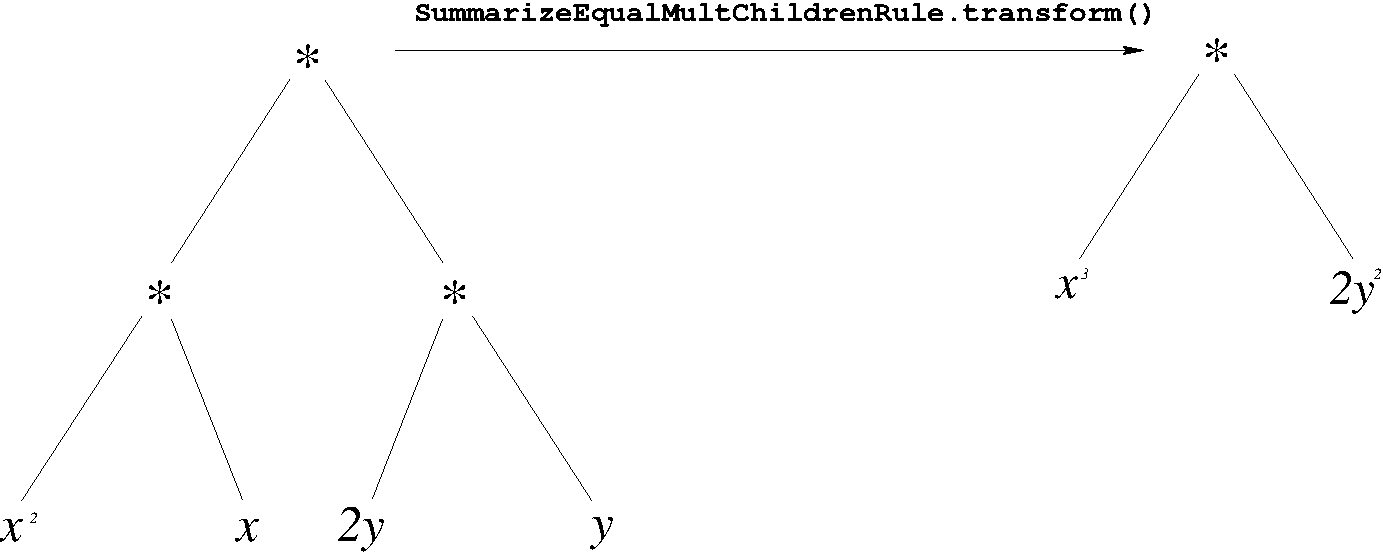
\includegraphics{diss_chapter/expressionTransform}}\nopagebreak\\[0.5cm]\nopagebreak
\scriptsize{{\sf Fig.\ \arabic{figcount}: Transformation of a subtree by a rule}}\\[0.6cm]
\end{center}

The {\tt OpTransform} object is a tree automaton that transforms trees by using a set of rules (located in the subpackage 
{\tt algebra.op.rule}), which specify a certain subtree pattern and a transformation that 
is performed if the tree matches the pattern.\\

For example, in the tree {\tt (* (* x$^2$ x) (* 2y y))} (see figure) the condition for a multiplication node containing two 
or more equal children (without regarding their factors or exponents) applies to both '{\tt *}' children of the root node. 
The rule object therefore raises the power of the first child by the number of the other children, transforming the tree 
to {\tt (* x$^3$ 2y$^2$)}. This would also apply to the root node if a previous application of {\tt CollapseEqualOpsRule} 
had flattened the tree to {\tt (* x$^2$ x 2y y)}.

In order to apply a rule like in the example above, a certain structure of the tree has to be assumed. For example, 
the tree {\tt (* (* (\^{} x 2)) x)} is mathematically equivalent to {\tt (* x$^2$ x)}, but it is harder to analyse and
transform. Because the rules should be kept as simple as possible (since there are many of them and their set should be 
easily expandable), it is reasonable to specify a normal form for operation trees.\\
The normalisation rules are located in {\tt algebra.op.rule.normalize}. Here are some examples:\\[0.3cm]

\begin{small}
\begin{tabular}{ll} 
Name & Application Example\\
{\tt NormalizeMultRule} & {\tt (* 4x 6y) $\rightarrow$ 24(* x y)}\\
{\tt NormalizeExponentsRule} & {\tt (* x$^4$ y$^6$) $\rightarrow$ (* x$^2$ y$^3$)$^2$}\\
{\tt CollapsePowerRule} &  {\tt  (\^{} (\^{} x y) z) $\rightarrow$ (\^{} x (* y z))}\\
{\tt HandleFunctionSymmetryRule} & {\tt (sin -x) $\rightarrow$ -(sin x)}\\
\end{tabular}\\[0.3cm]
\end{small}

This set can be easily expanded, most of the rules consist of less than 20 lines of code.
All the rules are applied in a deterministic order and since they always produce defined results, it can be ensured 
that after none of the rules can be applied to any node in the tree anymore, the operation has a unique defined form.
This form is defined as the normal form of the operation (for the specific rule-set). Trees having the same normal form 
are considered to be mathematically equal by the system.

\subsection{Object Model of Relations}
\paragraph{Generation and Structure of Relations}
Analogous to operations, relations are usually generated by parsing a word of {\it Rel} (see the grammar in 
\ref{rel_grammar}) and by constructing a relation tree composed of {\tt RelNode}s. The inner nodes of the relation tree 
are the logical operations 
$\vee$, $\wedge$ and $\neg$, while the leaves are either
simple relations (equations or inequations) or special nodes like {\tt AllRel} and {\tt NullRel}, which either relate 
everything (making interpretation of the used domain necessary) or nothing.

\paragraph{Transformation of Relations, Normal Form}
Like operations, relations can be transformed in multiple ways, the most used transformations are the logic
transformations that negate, conjunct or disjunct subtrees. But there are also complex transformations that occur when a
simple relation is transformed. For example, if the inequation $x^2 - x > 0$ is divided by $x$ this leads to the
equivalent complex relation\\ $x-1 > 0 \wedge \frac{1}{x} > 0 \vee x-1<0 \wedge \frac{1}{x} < 0$ (see figure).\\[0.3cm]
The functionality for handling relation transformations and its special cases are implemented in the class 
{\tt RelTransform}.\\

\stepcounter{figcount}
\begin{center}
\resizebox*{12cm}{!}{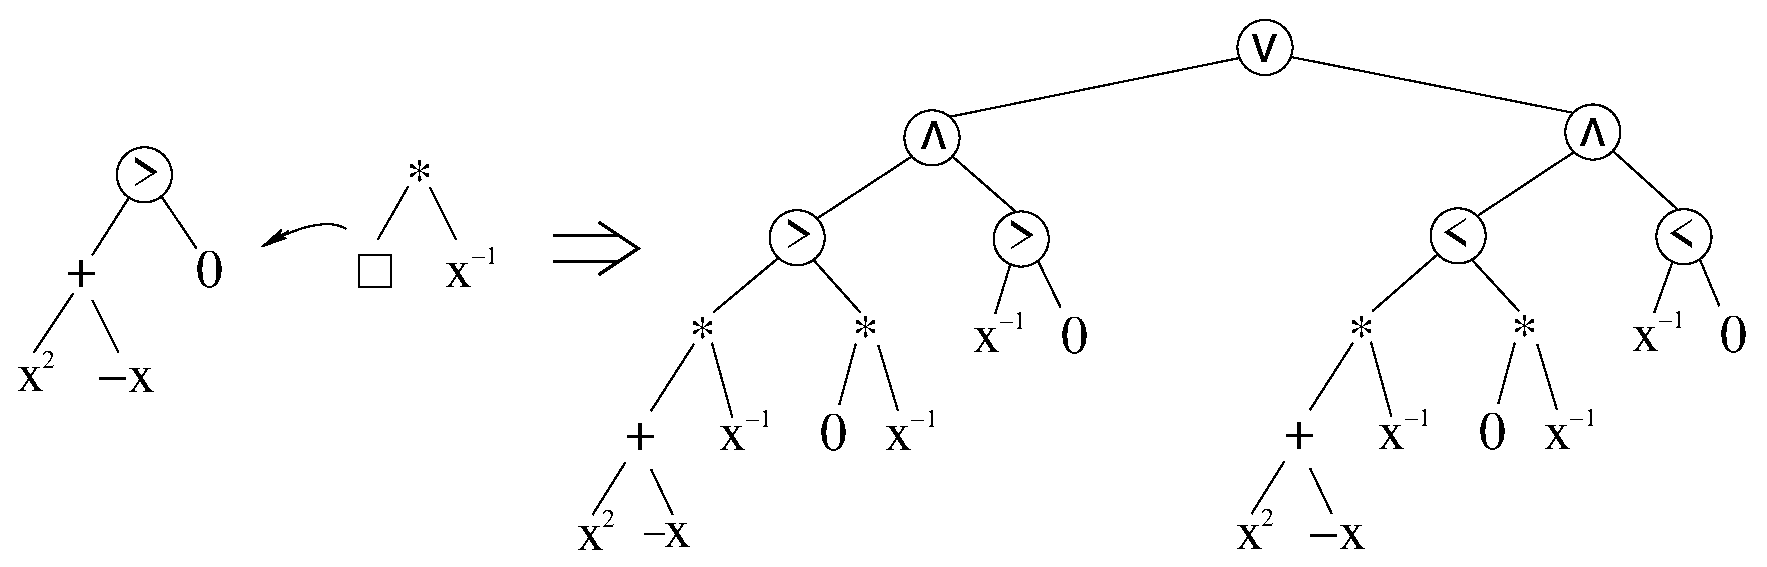
\includegraphics{diss_chapter/relationTransform}}\nopagebreak\\[0.5cm]\nopagebreak
\footnotesize{{\sf Fig.\ \arabic{figcount}: Transformation of a relation}}\\[0.6cm]
\end{center}

For comparation and simplification of relations, again, a higher order is needed for the trees to facilitate 
the development of tree analysis and transformation code.\\
For example, the relation $x = y \wedge y = x$ should be recognised as redundant by the system and be 
simplified to $x = y$. As for operation trees, this is done by defining a normal form for relations and
implementing rules for normalisation.\\ 
The normalisation rules are located in {\tt algebra.rel.rule.normalize}.
Here are some examples:\\[0.3cm]
\begin{small}
\begin{tabular}{ll} 
Name & Application Example\\
{\tt MoveOrUpwardsRule} &  {\tt [[x=0 OR y=0] AND z=0] $\rightarrow$ [x=0 AND z=0] OR [y=0 AND z=0]}\\
{\tt CollapseComplexRule} & {\tt [[x=0 AND y=0] AND [z=0] $\rightarrow$ [x=0 AND y=0 AND z=0]}\\
{\tt RemoveNotRelRule} & {\tt [NOT [x>=y]] $\rightarrow$ [x < y]}\\
\end{tabular}\\[0.3cm]
\end{small}


\section{Applications}\label{model_application}
To demonstrate the practical use of the algebraic object model, we give two application examples.

\paragraph{Symbolic Derivation}
The symbolic derivative of a differentiable function can be computed automatically by simply applying 
the well known rules for elementary functions and chaining them together for compound functions, using the
derivation rules for sums, products and compositions.\\


\stepcounter{figcount}
\begin{center}
\resizebox*{12cm}{!}{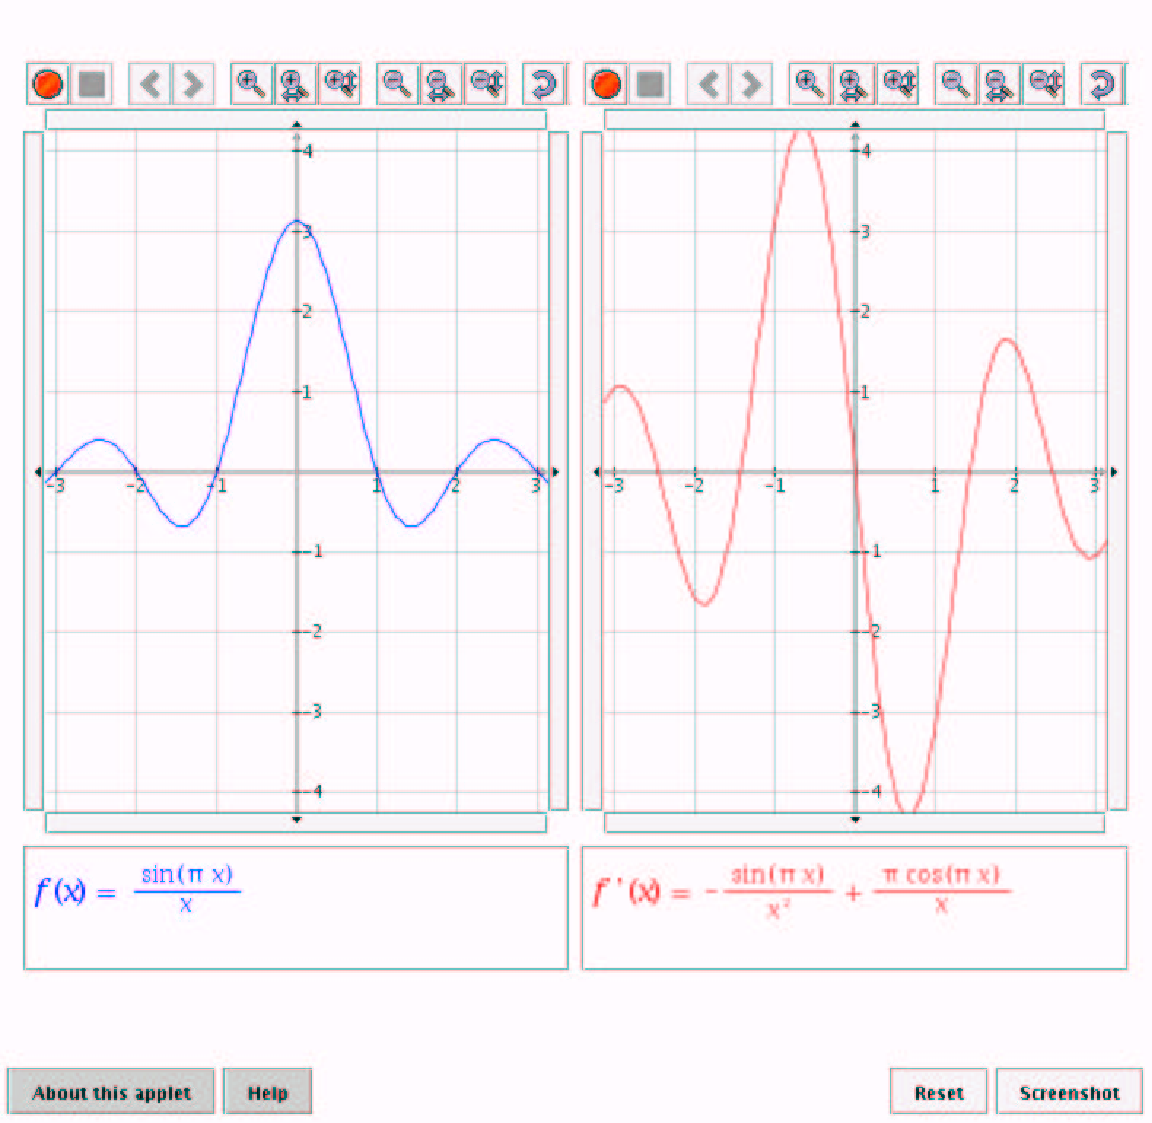
\includegraphics{diss_chapter/functionAndDerivative}}\nopagebreak\\[0.5cm]\nopagebreak
\footnotesize{{\sf Fig.\ \arabic{figcount}: The function and derivative plotter}}\\[0.6cm]
\end{center}

The application presented to the user is an applet that plots an arbitrary function typed in by the user and additionally
computes and displays the derivative (if any exists).\\[0.3cm]

\stepcounter{figcount}
\begin{center}
\resizebox*{6cm}{!}{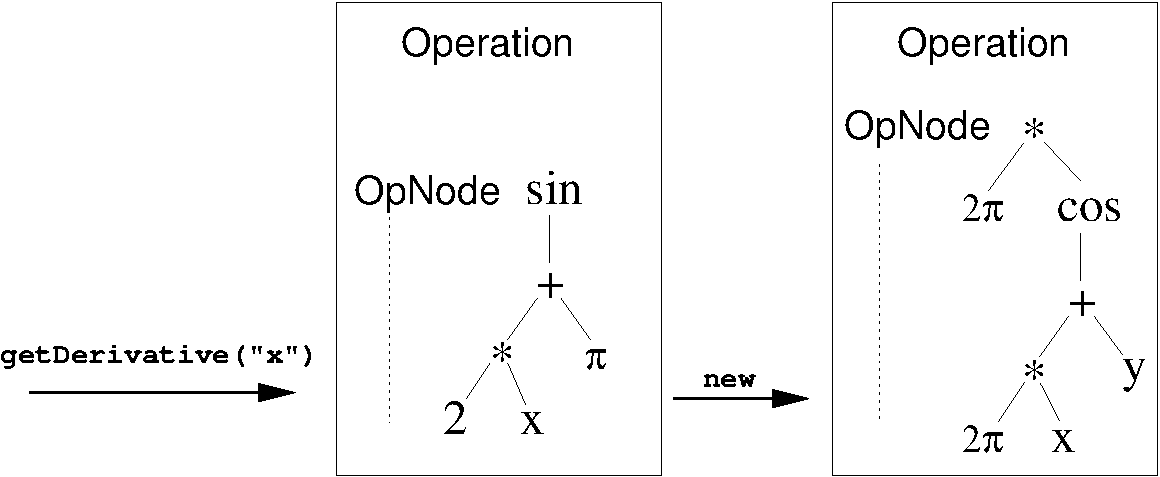
\includegraphics{diss_chapter/op_derive}}\nopagebreak\\[0.5cm]
\nopagebreak
\footnotesize{{\sf Fig.\ \arabic{figcount}: Object model for deriving operations}}\\[0.6cm]
\end{center}

From a technical perspective this is done by using an {\tt MMFunctionDefinedByOperation} object from which another instance 
is created with an {\tt Operation} that is returned by the {\tt getDerivative()} method of the first operation.\\
Deriving an operation can be implemented completely on a per-node basis, therefore the method {\tt Operation.getDerivative()} 
simply delegates the calculation to the root node of the operation tree. The derivation code of an operation node 
has two parts: a generic part that does the derivation for the internal factor and exponent and a specific part that 
varies on the node type. Below is a code snippet containing the node specific derivation code in the class 
{\tt SinOp}:\\[0.3cm]


\begin{minipage}{5cm}
\end{minipage}
\begin{minipage}{12cm}
\begin{scriptsize}
\begin{verbatim}
  /**
   *  Implements <i> (sin(f(x)))' = cos(f(x)) * f`(x) </i>.
   */
  public OpNode getDerivative(String variable){
    
    if(getMaxPowerOfVariable(variable) == 0)
      return new NumberOp(m_numberClass, 0);
    
    // cos(f(x))
    OpNode cosOp = new CosOp(m_numberClass);
    cosOp.setChildren(new OpNode[]{(OpNode)(m_children[0].clone())});
    
    // f'(x)
    OpNode derivedChild = m_children[0].getDerivative(variable);
    
    // cos(f(x)) * f'(x)
    MultOp derivedCosOp = new MultOp(m_numberClass);
    derivedCosOp.setChildren(new OpNode[]{cosOp, derivedChild});
    return deriveNode(derivedCosOp);
  }
\end{verbatim} 
\end{scriptsize}
\end{minipage}\\[0.3cm]

The generic part implemented in the abstract class {\tt OpNode} is as follows\\

\begin{minipage}{5cm}
\end{minipage}
\begin{minipage}{12cm}
\begin{scriptsize}
\begin{verbatim}
  /**
   *  Implements <i>(m*a(x)^n)' = (n*a(x) ^ (n-1) * m*a'(x)</i>.
   *  @param derivedNode a'(x)
   */
  protected OpNode deriveNode(OpNode derivedNode){
    if(m_exponent == 1){
      derivedNode.setFactor(m_factor.copy());
      return derivedNode;
    }
    MultOp derivedPower = new MultOp(m_numberClass);
    OpNode newPower = (OpNode)clone();
    newPower.m_factor.mult(NumberFactory.newInstance(m_numberClass, m_exponent));
    newPower.m_exponent--;
    derivedPower.setChildren(new OpNode[]{newPower, derivedNode});
    return derivedPower;
  }
\end{verbatim} 
\end{scriptsize}
\end{minipage}\\[0.3cm]


\paragraph{Definition Range of Operations}
\label{definition_range_operations}
Another useful application of the MathletFactory algebraic object model is the ability to compute the definition 
range of an operation. We have used this functionality to add an extra warning when displaying mathematical entities
that use operations which are only partially defined.\\
When determining definition gaps, it poses a serious implementation problem to numerically calculate the complete 
definition range and display it graphically for any function (as the example $f(x) =  \frac{1}{\sin(\frac{1}{x})}$ in the
figure below shows).\\
The MathletFactory addresses this problem by displaying the definition range of a function as a symbolic expression. 
Though this expression often has an implicit form (showing only a relation of the used variables that must be satisfied) 
the user is warned of existing definition gaps, and he is principally able to find out where they are.\footnote{Also, by 
using the {\tt Relation.toContentMathML()} export method, an application programmer is able to link it with a computer algebra 
system or to implement a numerical solution of his own.}\\[0.3cm]

\stepcounter{figcount}
\begin{center}
\resizebox*{8cm}{!}{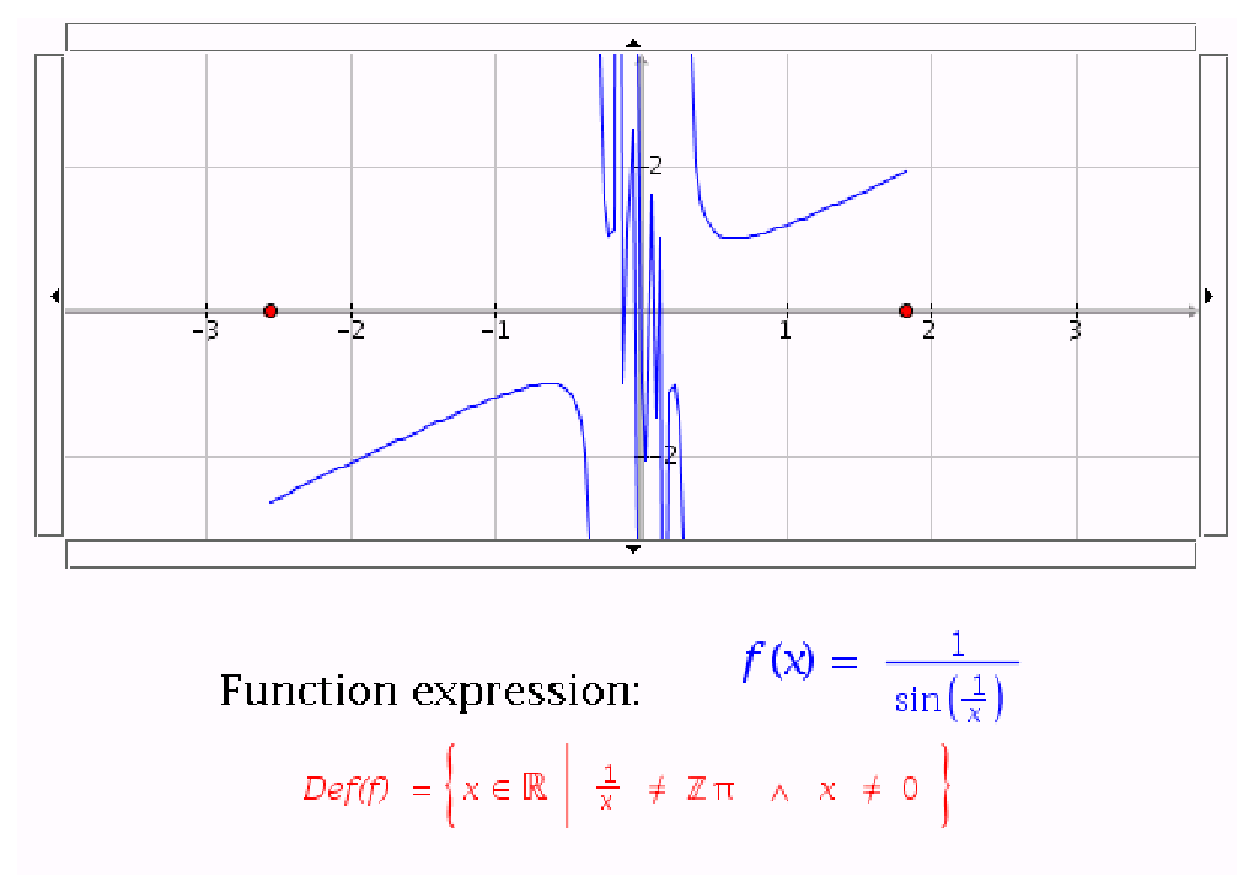
\includegraphics{diss_chapter/simplefunctionplotter2}}\nopagebreak\\[0.5cm]\nopagebreak
\footnotesize{{\sf Fig.\ \arabic{figcount}: The function plotter with definition range detector}}\\[0.6cm]
\end{center}

From the technical perspective the computation of the definition range for an arbitrary operation is also solved on a
per-node basis. By calling the method {\tt getDefinedRel()} the {\tt OpNode} object creates a {\tt RelNode} object which
represents a relation that a member of the definition range for the operation must satisfy. 
The {\tt RelNode}s of the children of an {\tt OpNode} are connected by an {\tt AndRel} conjunction, forming a relation tree
that is at last anchored in a {\tt Relation} object by the enclosing {\tt Operation.getDefinedRelation()} method.
For the {\tt OpNode}s there is -- like the computation of the derivative -- a generic and a node-specific implementation.
The generic part, implemented in {\tt OpNode} is as follows:\\[0.3cm]

\begin{minipage}{5cm}
\end{minipage}
\begin{minipage}{12cm}
\begin{scriptsize}
\begin{verbatim}
  /**
   * Returns the relation for which the operation represented by this node is defined.
   * @see #getDefinedRel(OpNode operand)
   */
  public RelNode getDefinedRel(){
    
    // by default the operation is defined totally for any variable
    RelNode definedRel = new AllRel(m_numberClass);
    
    // retrieve the definition range of this node with the child as argument
    // (non unary operations overload this method)
    if(m_children != null)
      definedRel = getNodeDefinedRel(m_children[0]);
      
    // for nodes with a negative exponent the base may not become zero
    if(getExponent() < 0){
      OpNode nodeWithoutExponent = (OpNode)clone();
      nodeWithoutExponent.setExponent(1);
      definedRel = new AndRel(definedRel, new NotRel(nodeWithoutExponent.getZeroRel()));
    }    
    
    // intersect the defintion range of this node with the definion range of the children 
    if(m_children == null)
      return definedRel;
    else
      return new AndRel(definedRel, getChildrenDefinedRel()); 
  }

  /**
   * Returns the relation subtree for which this operation with 
   * <code>operand</code> as child is defined. It does not consider the 
   * exponent of this node, which is be checked in {@link #getDefinedRel}.
   */
  public abstract RelNode getNodeDefinedRel(OpNode operand);
\end{verbatim} 
\end{scriptsize}
\end{minipage}\\[0.3cm]
The specific part is implemented by the subclasses of {\tt OpNode} in {\tt getNodeDefinedRel()}. Here is an example for 
{\tt TanOp} returning a relation that says that the cosine of its operand may not be zero:\\[0.3cm]
\begin{minipage}{5cm}
\end{minipage}
\begin{minipage}{12cm}
\begin{scriptsize}
\begin{verbatim}

  public RelNode getNodeDefinedRel(OpNode operand){
    return new NotRel(new CosOp(m_numberClass).getZeroRel((OpNode)operand.clone()));
  }

\end{verbatim} 
\end{scriptsize}
\end{minipage}\\[0.3cm]

\section{Arithmetic and Geometric Symbolic View Architecture}
One pattern that has been consequently used in the development of the symbolic view architecture is, that every
mathematical inclusion is transformed to a `containedness' relation on the view component level. This allows an
easy development and support for a multitude of symbolic representations. We illustrate this with the example
of constructing the parametric view for an affine plane in $\mathbbm{R}^3$:

\stepcounter{figcount}
\begin{center}
\resizebox*{6cm}{!}{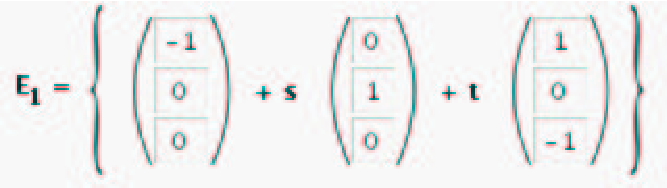
\includegraphics{diss_chapter/plane_symbolic}}\hspace{1cm}\resizebox*{5.5cm}{!}{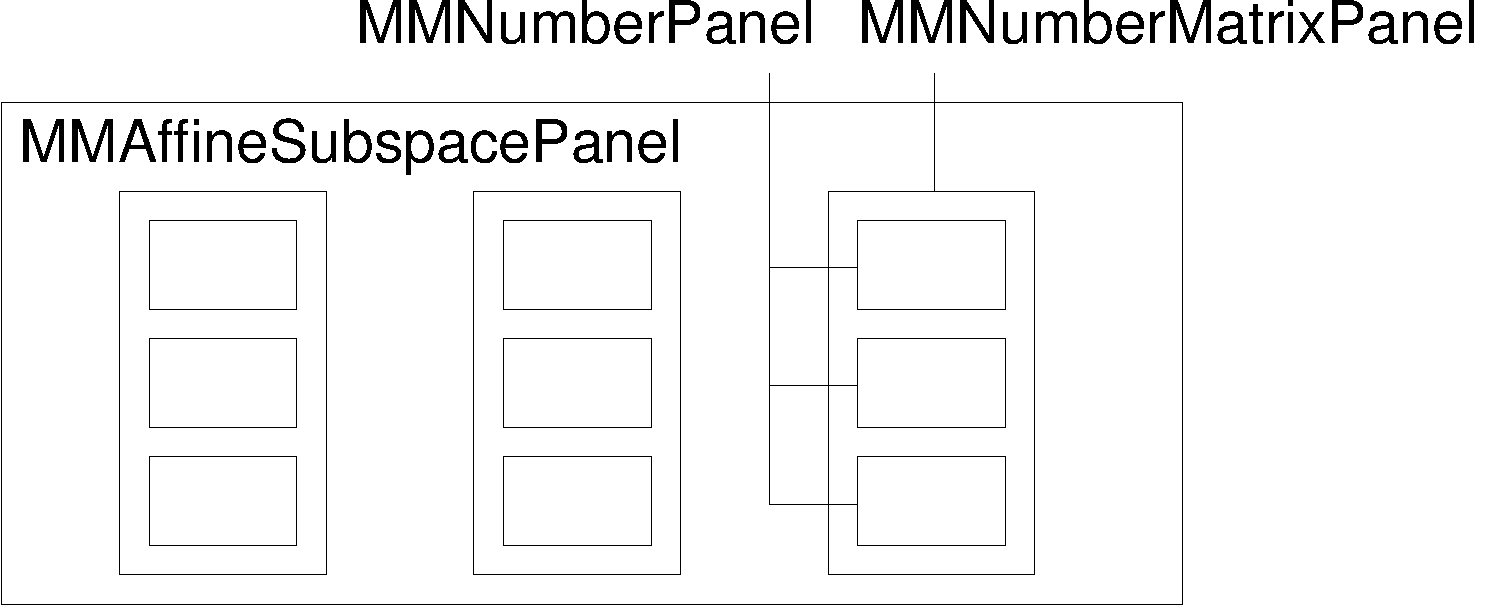
\includegraphics{diss_chapter/plane_symbolic_structure}}\nopagebreak\\[0.3cm]\nopagebreak
\footnotesize{{\sf Fig.\ \arabic{figcount}: The symbolic view of a plane and its structure}}\\[0.6cm]
\end{center}

On Java level, the view is simply a subclass of {\tt JPanel}, namely an {\tt MMAffineSubspacePanel}. This class
acts not only as a view for a plane in $\mathbbm{R}^3$, but also for a line or point in $\mathbbm{R}^3$ or in 
$\mathbbm{R}^2$, thus making it possible to use it as a view of a dynamically generated affine subspace (like the
intersection or join of other affine spaces). But let us first consider, that it displays a regular (non-degenerated)
plane. In this case, we need to display three vector displays: one displaying the origin vector and two for the 
direction vectors. This is simply done by adding three {\tt MMNumberMatrixPanel}s, which is the standard display
component for a vector of any dimension, but also of course for any number matrix of arbitrary form. These panels
in turn contain all entries as {\tt MMNumberPanel}, the symbolic representation for numbers of any 
type.\footnote{Note, that the inclusion does not end there, for the number panel itself contains an operation panel 
(see below) to allow the display of constants like $\frac{3}{2}pi$, etc.} A simple update mechanism using the Java 
property support ensures, that changes performed by the user are recorded by the master MMObject. On the other hand, 
if the mathematical state of the MMObject changes (e.g.\ by updating or user interactions on the graphical level), 
the changes are immediately displayed, allowing the user to continuously watch the symbolic perspective of his 
actions.\\
This applies not only to changing the vectors of the affine subspace, but also to changing its dimension: If the
plane was the result of an intersection of two other planes (which were geometrically identical) and one of these 
planes changed, making the intersection a line or an empty space, the symbolic view adapts to these cases without
complaints.

\section{Algebraic Symbolic View Architecture}
In the following, we will also sketch the view architecture used by the MathletFactory's algebraic object model, 
for details the commented source code and API documentation should be consulted.\\
The architecture for symbolically displaying algebraic entities is closely related to the structure of the algebraic 
object model: A tree of operation nodes is mapped on a tree of view nodes that recursively draw the expression on a 
panel, whereas a tree of relation nodes is mapped on a tree of panels with each parent containing its children.

\subsection{View Architecture of Operations}
\label{view_model}
The implementation of the symbolic view for an operation is the {\tt OperationPanel}. This is a GUI component that 
draws the expression string on its screen area when asked to repaint. This is done by view nodes (an analogon to the 
\TeX{} noads\footnote{\cite{Kn82}}), each of which corresponds to an operation node of the {\tt Operation}. Apart from 
the reference to its operation node, a view node keeps track of its metrics which is determined by the metrics of its 
children (if any) and the font of the panel. For example, the view node for a square root must know the width and height 
of its child expression in order to fully enclose the radicand (see figure).\\
So when a repaint event is sent to the operation panel, the panel asks its root view node to draw itself on the panel.
If the root view node has children, it asks them to calculate their metrics (which in turn may depend on their children�s
metrics, etc.) and then draws the expression it represents accordingly.\\

\stepcounter{figcount}
\begin{center}
\resizebox*{6cm}{!}{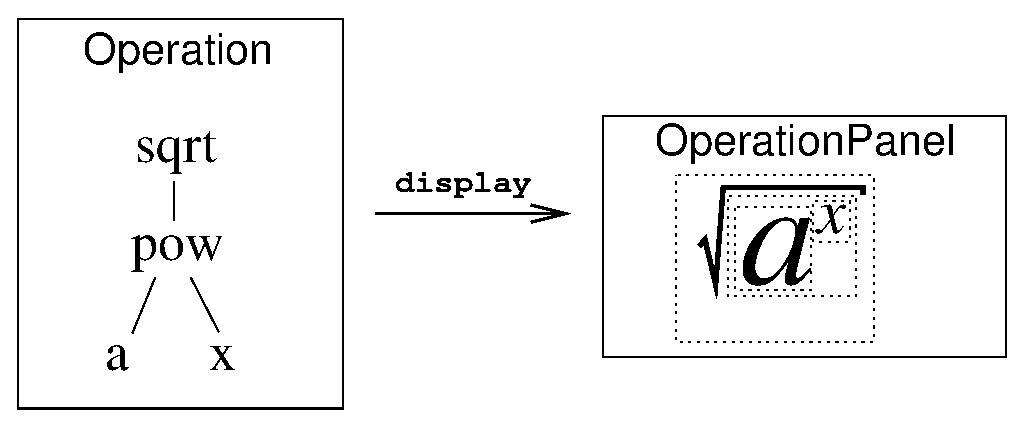
\includegraphics{diss_chapter/opView}}\nopagebreak\\[0.5cm]\nopagebreak
\footnotesize{{\sf Fig.\ \arabic{figcount}: Displaying operations, the dashed lines mark the {\tt OpViewNode}s that draw on the {\tt OperationPanel}.}}\\[0.6cm]
\end{center}

\subsection{View Architecture of Relations}
The inclusion of operations in relations can also be transferred to the view architecture: The view component for a simple
relation, a {\tt SimpleRelationPanel} is merely a panel containing two {\tt OperationPanel}s with a relation sign label 
between them. Complex relations are displayed by instances of {\tt RelationContainer}: Panels that contain either 
{\tt SimpleRelationPanel}s or other {\tt RelationContainer}s. The root node itself is contained in a component called
{\tt RelationPanel}.\\

\stepcounter{figcount}
\begin{center}
\resizebox*{6cm}{!}{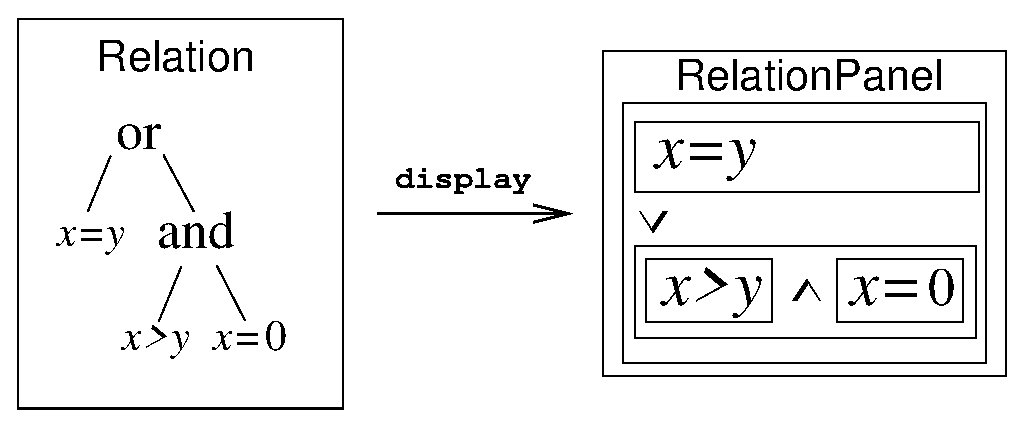
\includegraphics{diss_chapter/relView}}\nopagebreak\\[0.5cm]\nopagebreak
\footnotesize{{\sf Fig.\ \arabic{figcount}: Relation trees are rendered in a container hierarchy rooted by an {\tt RelationPanel}.}}\\[0.6cm]
\end{center}

\subsection{Metrics of View Components}
The MathletFactory uses the standard metrics model of typography\footnote{\cite{He93}}: The metrics of each glyph is 
characterised by its width, ascent and descent; for the rendering of fractions, sub- and superscripts the baseline must 
also be recorded. Operation view nodes keep their metrics parameters in an object called {\tt ViewNodeMetrics}. 
On the panel level (anything that uses {\tt OperationPanel}s or container trees of these) this is done by implementing 
the interface {\tt Alignable}, which declares methods for retrieving the metrics parameters. By using this interface it is 
ensured that two operations can be horizontally aligned (i.e.\ having the same baseline), even if they have different 
heights or one of them has a border (e.g.\ for marking it as editable).\\

\stepcounter{figcount}
\begin{center}
\resizebox*{8cm}{!}{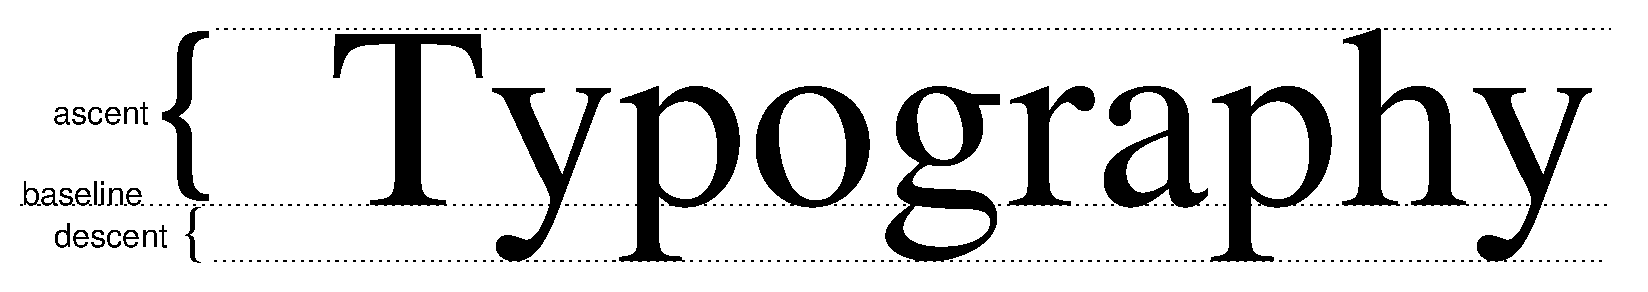
\includegraphics{diss_chapter/typo}}\nopagebreak\\[0.5cm]\nopagebreak
\footnotesize{{\sf Fig.\ \arabic{figcount}: The baseline, ascent and descent of a font.}}\\[0.6cm]
\end{center}

\section{Graphical View and Controller Architecture}

At the time of writing, implementations for the Java2D system library and the Java3D API exist, but previous prototype 
implementations have also been tested with the third party graphics library JavaView\footnote{\cite{JV04}}. The 
architecture works as follows: For each different display type there exists a specific canvas (a subclass of 
{\tt MMCanvas}) that can be added to an applet like any other GUI component. If an application programmer wants to display 
a certain MMObject, he simply calls {\tt addObject(MMObjectIF object)} in the canvas with the MMObject as argument and the 
systems automatically assigns the appropriate (or a previously chosen) visual representation.\\

\stepcounter{figcount}
\begin{center}
\resizebox*{7.5cm}{!}{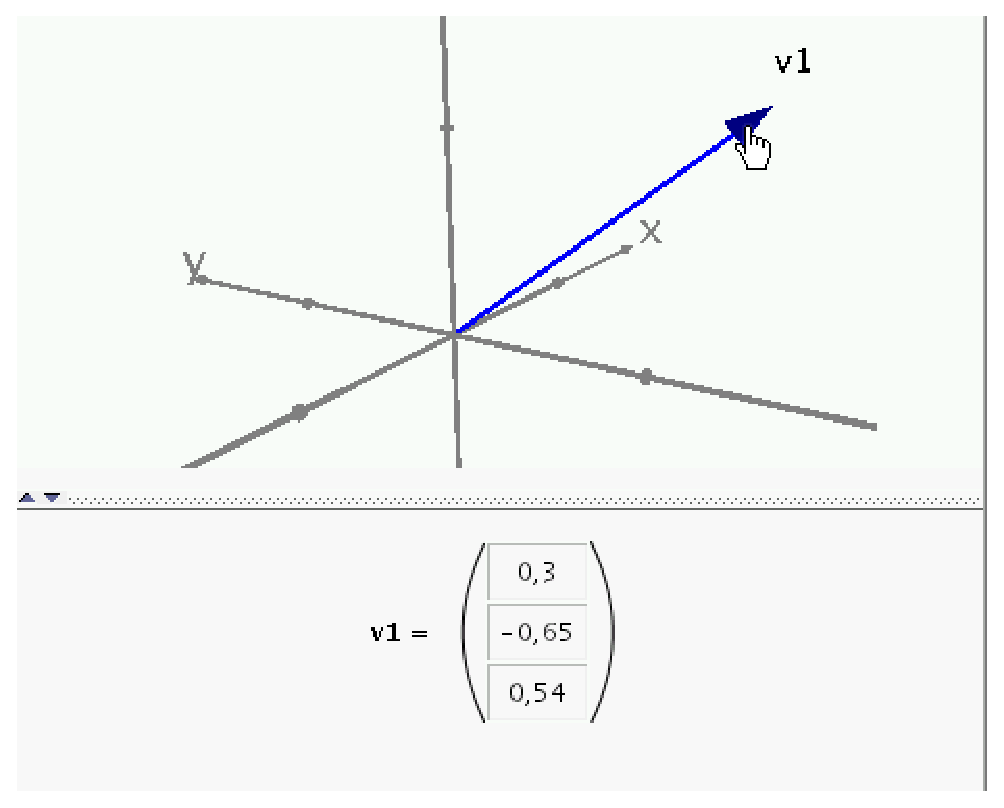
\includegraphics{diss_chapter/3d_vector}} \hspace{1.5cm}
\resizebox*{7.5cm}{!}{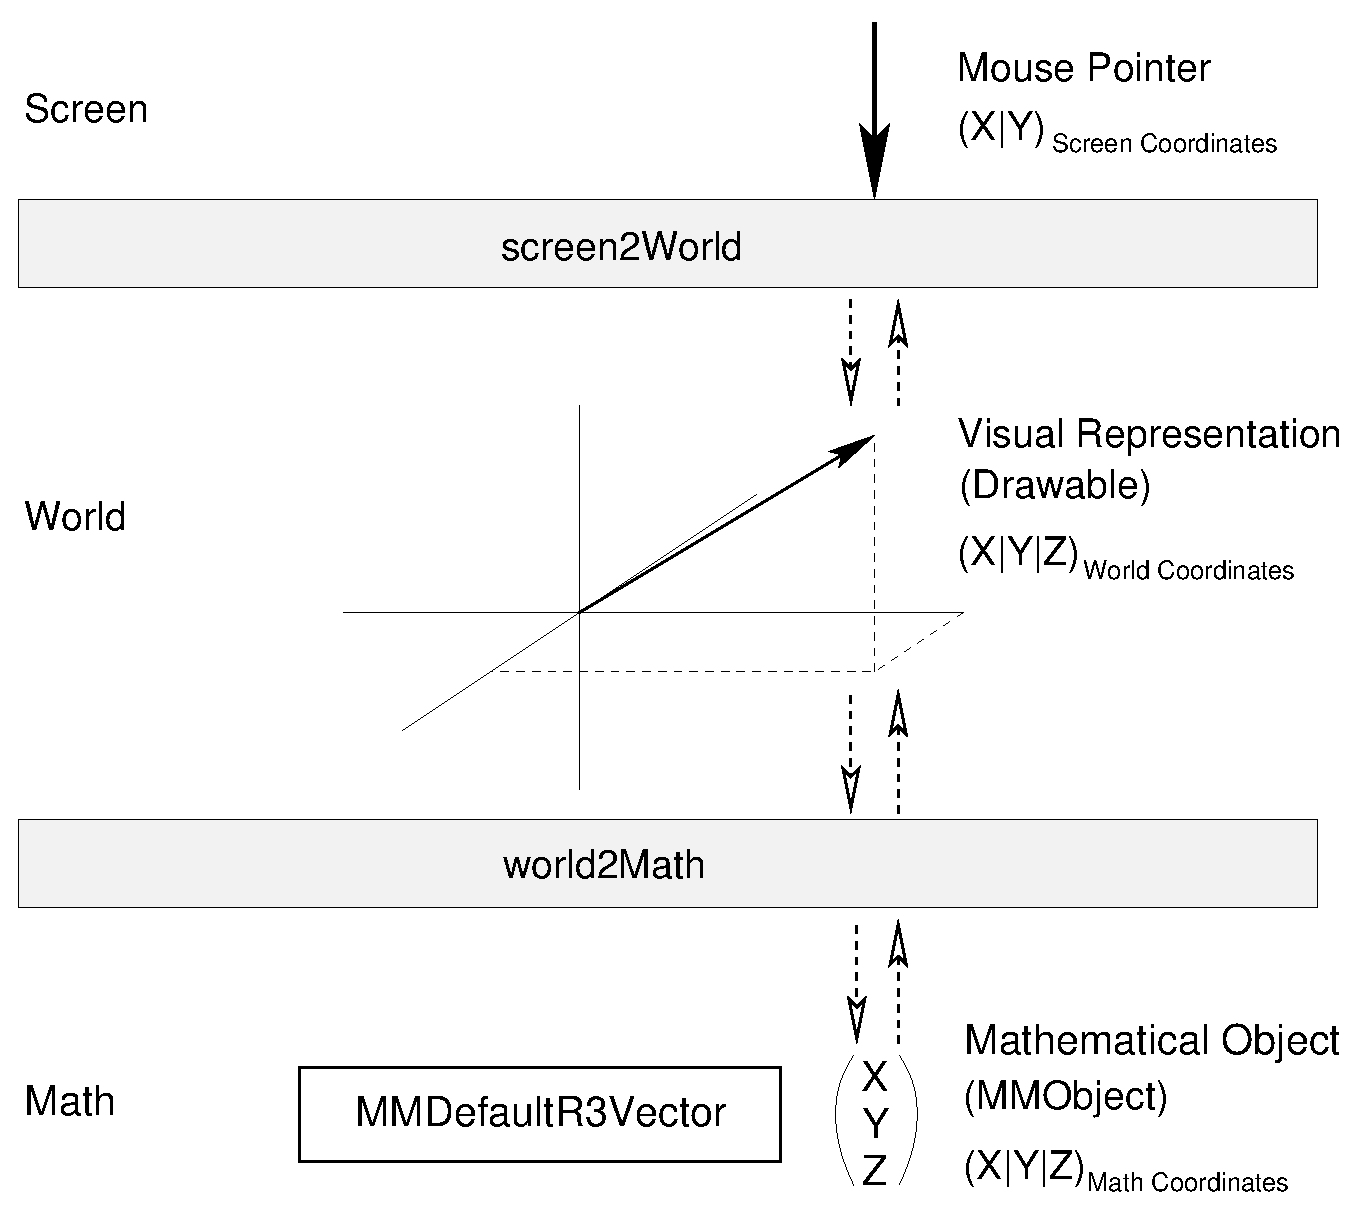
\includegraphics{diss_chapter/vector_drag}}\nopagebreak\\[0.5cm]\nopagebreak
\footnotesize{\sf Fig.\ \arabic{figcount}: Dragging a 3D vector: How the display and interaction system works}\\[0.6cm]
\end{center}

For example, when a user drags the end point of a 3D vector with the mouse, the mouse coordinates (measured in pixels) 
are transformed by a matrix {\tt screen2World} into world coordinates. These describe a virtual space, where the visual 
representations of mathematical objects `live'. The mathematical objects themselves reside in a separate coordinate space 
called the math space. This allows them to be independent of the worlds geometry and dimension, thus allowing, for example, 
projections from a spherical geometry into the euclidian world coordinate space. For euclidian math spaces the 
transformation is simply done by another matrix called {\tt world2Math}. So when the user drags the vector, the mouse 
coordinates are transformed into world and math coordinates. The object's coordinates are changed and the graphical view 
updates accordingly, allowing further interaction. For 2D (or 1D) vectors the mechanism is the same.\\

We have given only a short overview of a complex system; yet, an application developer needs not know about all this, 
because there is a large set of prefabricated {\it handlers} that implement almost all desired functionality for 
manipulating MMObjects. So if an application developer wants to construct a mathlet, where the user may drag a vector (or 
any other MMObject), he only has to add the appropriate handler to it.

\begin{thebibliography}{100}  

\bibitem[ASU86]{ASU86} A: Aho, R. Sethi, J. Ullman. Compilers - Principles, Techniques and Tools. Addison Wesley. 1996.

\bibitem[Bau02]{Bau02} C. Bauer, A. Frink, R. Kreckel.\\
Introduction to the GiNaC Framework for Symbolic Computation within the C++ Programming Language.\\
Journal of Symbolic Computation Volume 33, Number 1, 2002.

\bibitem[Bu96]{Bu96} F. Buschmann et al. Pattern-Oriented Software Architecture, Volume 1: A System of 
Patterns. Addison-Wesley 1996.

\bibitem[Co03]{Co03} H. Comon et al. Tree Automata Techniques and 
Applications. Preprint, 2003.\\ {\footnotesize {\sf http://www.grappa.univ-lille3.fr/tata}}

\bibitem[He93]{He93}  R. Hersch (Ed.). Visual and Technical Aspects of Type. Cambridge University Press. 1993.

\bibitem[HU79]{HU79}J.E. Hopcroft and J.D. Ullman. Introduction to Automata
Theory, Languages and Computation. Addison Wesley. 1979.

\bibitem[JV04]{JV04} JavaView homepage. 2004.\\
{\footnotesize {\sf http://www.javaview.de}}

\bibitem[Kn82]{Kn82} D. Knuth. Documented \TeX{} source code. 1982.\\
{\footnotesize {\sf http://www.ctan.org/tex-archive/systems/knuth/tex/tex.web}}. 

\bibitem[Mo93]{Mo93} K. Morisse. Datenstrukturen und Speicherverwaltung in MuPAD. In: 
mathPAD Vol. 3 No. 2. 1993.\\
{\footnotesize {\sf http://www.mupad.de/mathpad.shtml}}

\bibitem[Wa91]{Wa91} Maple Language Reference Manual. Waterloo Maple Publishing. 1991.

\bibitem[Wo91]{Wo91} S. Wolfram. The Mathematica Book. Cambridge. 1991.

\end{thebibliography}

\clearpage

\chapter{Miscellaneous Topics}
\section{Commands for embedding applets in websites}
  It is possible to embed applets in websites via the traditional (and even deprecated)
  \verb|<applet>|-tag or via the recommended \verb|<object>|-tag.\\
  Below is a template for an \verb|<object>|-tag:\\
  \begin{verbatim}
    <object classid="java:MyApplet.class" codetyte="application/java"
          codebase="./" archive="MyApplet.jar" width="400" height="300">
      <param name="parameter1" value="...value...">
      <param name="parameter2" value="...value...">
    </object>
  \end{verbatim}
  Overview of attributes:
  \begin{itemize}
  \item \verb|classid| specifies the name of the applet with prefix "java:" and suffix ".class". Note that no path must be specified!
  \item \verb|codebase| specifies the path to the class-file relative to the HTML page's location
  \item \verb|archive| specifies a comma-separated list of needed archive files (e.g. zipped 
  libraries where also the applet class can be located)
  \end{itemize}

\section{Table: DisplayProperties in MMObjects and Drawables}
  {\small\ttfamily
  \begin{tabular}{|l|l|l|} \hline
    \rmfamily Properties-Class & \rmfamily implementing MM-Class & \rmfamily using Drawable\\ \hline\hline
    LineDisplayProperties & MMAffine2DLine & G2DLineDrawable\\
    & MMAffine2DLineSegment & J3DLineSegmentDrawable\\
    & MMAffine2DRay & J3DPolyLineDrawable\\
    & MMAffine3DLine & \\
    & MMAffine3DLineSegment & \\
    & MMCoordinateSystem & \\
    & MMDefaultRNVector & \\
    & MMVectorField2DOverR2- & \\
    & \indent\indent DefByComponents & \\
    & MMVectorField2DOverR2- & \\
    & \indent\indent DefByExpression & \\ \hline
    
    PointDisplayProperties & MMAffine2DPoint & G2DPointDrawable\\
    & MMAffine3DPoint & J3DPointDrawable\\
    & MMDefaultRN & \\
    & MMBezierPolynomialAdvanced & \\ \hline
    
    PolygonDisplayProperties & MMAffine2DPolygon & G2DPolygonDrawable\\
    & MMFunctionDefByOp & \\
    & MMFunctionDefinedByExpression & \\
    & MMFunctionDefinedBySamples & \\
    & MMPiecewiseFunction & \\
    & MMStepFunction & \\
    & MMBezierPolynomialAdvanced & \\
    & MMPolynomial & \\
    & MMParametricFunctionInR2 & \\
    & MMOneChainInR2 & \\ \hline
    
    SurfaceDisplayProperties & MMFunctionOverR2 & \rmfamily(no explicit drawable)\\
    & MMParametricFunctionInR3 & \\ 
    & MMAffine3DPlane & \\ 
    & MMAffine3DSubspace & \\ \hline
  \end{tabular}
  }
  
  \clearpage
  
  \section{Classes and their locations/packages}
  This section lists the most used classes with their location inside the library.
  All following package descriptions must have the explicit prefix  
  \verb|net.mumie.mathletfactory|.\\\\
  {\small\ttfamily
  \begin{longtable}{l | l}
    \rmfamily Class & \rmfamily Package\\ \hline\hline
    \endhead
    ActionManager & action\\
    Affine2DKeyboardGridTranslateHandler & action.handler\\
    Affine2DKeyboardTranslateHandler & action.handler\\
    Affine2DMouseGridTranslateHandler & action.handler\\
    Affine2DMouseTranslateHandler & action.handler\\
    Affine3DKeyboardTranslateHandler & action.handler\\
    Affine3DMouseTranslateHandler & action.handler\\
    AffineLineSegmentBetweenPointsUpdater & action.updater\\
    Animation & uitl.animation\\
    AnimationDependencyAdapter & uitl.animation\\
    AnimationDependencyUpdater & uitl.animation\\
    \\
    BaseApplet & appletskeleton\\
    BasicApplicationFrame & util\\
    \\
    CanvasControllerIF & action\\
    CanvasImage & util\\
    CanvasMessage & util\\
    Canvas2DObjectTransformer & transformer\\
    Canvas3DObjectTransformer & transformer\\
    ContainerObjectTransformer & transformer\\
    ControlPanel & appletskeleton.util\\
    \\
    DefaultCanvasController & action\\
    DependencyAdapter & action.updater\\
    DependencyUpdater & action.updater\\
    DisplayProperties & display\\
    \\
    FunctionAndDerivativeOverRIF & math.analysis.function\\
    FunctionOverBorelSetIF & math.analysis.function\\
    FunctionOverRIF & math.analysis.function\\
    \\
    GeneralTransformer & transformer\\
    \\
    LinearMap & math.algebra.linalg\\
    LinearMapDefByVectorsUpdater & action.updater\\
    LineDisplayProperties & display\\
    \\
    MathUtilLib & math.util\\
    MatrixLayout & appletskeleton.util\\
    MMAffine2DEllipse & mmobject.geom.affine\\
    MMAffine3DEllipse & mmobject.geom.affine\\
    MMAffine2DLine & mmobject.geom.affine\\
    MMAffine3DLine & mmobject.geom.affine\\
    MMAffine2DLineSegment & mmobject.geom.affine\\
    MMAffine3DLineSegment & mmobject.geom.affine\\
    MMAffine2DPoint & mmobject.geom.affine\\
    MMAffine3DPoint & mmobject.geom.affine\\
    MMComplex & mmobject.number\\
    MMComplexRational & mmobject.number\\
    MMCoordinateSystem & mmobject.geom.affine\\
    MMDefaultCanvasObject & mmobject\\
    MMDefaultObject & mmobject\\
    MMDouble & mmobject.number\\
    MMEditablePanel & display.noc\\
    MMEquationSystem & mmobject.algebra\\
    MMFunctionDefByOp & mmobject.analysis.function\\
    MMFunctionDefinedByExpression & mmobject.analysis.function\\
    MMFunctionDefinedBySamples & mmobject.analysis.function\\
    MMFunctionPanel & display.noc.function\\
    MMG2DCanvas & display.g2d\\
    MMInteger & mmobject.number\\
    MMInterval & mmobject.set\\
    MMJ3DCanvas & display.j3d\\
    MMNumberMatrix & mmobject.algebra.linalg\\
    MMNumberMatrixPanel & display.noc.matrix\\
    MMNumberPanel & display.noc.number\\
    MMNumberSet & mmobject.set\\
    MMNumberTuple & mmobject.algebra.linalg\\
    MMObjectIF & mmobject\\
    MMOpMatrix & mmobject.algebra.linalg\\
    MMPanel & display.noc\\
    MMPiecewiseFunction & mmobject.analysis.function\\
    MMPolynomial & mmobject.algebra.poly\\
    MMRational & mmobject.number\\
    MMRelation & mmobject.algebra\\
    MMSetDefByRel & mmobject.set\\
    MMString & mmobject.util\\
    MMStringMatrix & mmobject.util\\
    MumieTheme & appletskeleton.util\\
    \\
    NoCanvasApplet & appletskeleton\\
    NumberFactory & math.number\\
    NumberMatrix & math.algebra.linalg\\
    NumberTuple & math.algebra.linalg\\
    NumberTypeDependentIF & math.number\\
    \\
    OneChainInRIF & math.analysis.function\\
    OneChainInRNIF & math.analysis.function.multivariate\\
    Operation & math.algebra.op\\
    OperationPanel & display.noc.op\\
    OpMatrix & math.algebra.linalg\\
    OpParser & math.algebra.op\\
    OpTuple & math.algebra.linalg\\
    \\  
    PointDisplayProperties & display\\
    PolygonDisplayProperties & display\\
    Progress & util.animation\\
    PropertyHandlerIF & mmobject\\
    \\
    Relation & math.algebra.rel\\
    RelParser & math.algebra.rel\\
    \\
    SequenceAdapter & math.analysis.sequence\\
    SequenceIF & math.analysis.sequence\\
    SeriesIF & math.analysis.sequence\\
    SideBySideG2DCanvasApplet & appletskeleton.g2d\\
    SideBySideJ3DCanvasApplet & appletskeleton.j3d\\
    SingleG2DCanvasApplet & appletskeleton.g2d\\
    SingleJ3DCanvasApplet & appletskeleton.j3d\\
    SpecialCaseEvent & action.message\\
    SpecialCaseListener & action.message\\
    Step & util.animation\\
    SurfaceDisplayProperties & display\\
    \\
    TabbedPanel & appletskeleton.util\\
    TextLayout & appletskeleton.util\\
    TextPanel & appletskeleton.util\\
    \\
    UpperLowerG2DCanvasApplet & appletskeleton.g2d\\
    UpperMiddleLowerG2DCanvasApplet & appletskeleton.g2d\\
    UsesOpArrayIF & math.algebra.op\\
    UsesOperationIF & math.algebra.op\\
    UsesRelationIF & math.algebra.rel
    \\
    VectorField2DOverR2IF & math.analysis.vectorfield\\
    VectorFunctionOverBorelSetIF & math.analysis.function.multivariate\\
    VectorFunctionOverDomainIF & math.analysis.function.multivariate\\
    VectorFunctionOverRIF & math.analysis.function.multivariate
    
  \end{longtable}
  }
  

%%%%%%%%%%%%%%%%%%%%%%%%%%%%%%%%%%%%%%%%%%%%%%%%%%%%%%%%%%%%%%%%%%%%%%%%%%%%%%%%%%%%%%%%%%%%%%%%
\clearpage

\section{Code: TriangleAltitude-Applet}
\begin{footnotesize}
\begin{verbatim}
<...> // some imports omitted

public class TriangleAltitude extends SingleG2DCanvasApplet{
  
  private MMAffine2DPoint A, B, C;
  private MMAffine2DLineSegment AB, BC, CA;
  private MMAffine2DLineSegment aFootC, bFootA, cFootB, bFootC, cFootA, aFootB;
  private MMAffine2DLineSegment altitude_AB, altitude_BC, altitude_CA;
  
  private PointDisplayProperties pp;
  private LineDisplayProperties ll, kk, mm;
  
  private Affine2DKeyboardTranslateHandler akth;
  private Affine2DMouseTranslateHandler amth;
  
  public void init() {
    setTitle("Triangle Altitude Test");
    createObjects();
    initializeObjects();
    createDependencies();

    getCanvas().addObject(aFootC);
    getCanvas().addObject(bFootC);
    getCanvas().addObject(bFootA);
    getCanvas().addObject(cFootA);
    getCanvas().addObject(cFootB);
    getCanvas().addObject(aFootB);
    getCanvas().addObject(altitude_AB);
    getCanvas().addObject(altitude_BC);
    getCanvas().addObject(altitude_CA);
    getCanvas().addObject(AB);
    getCanvas().addObject(BC);
    getCanvas().addObject(CA);
    getCanvas().addObject(A);
    getCanvas().addObject(B);
    getCanvas().addObject(C);
    
    addResetButton();
    addScreenShotButton();
  }
  
  private void createObjects() {
    amth = new Affine2DMouseTranslateHandler(getCanvas());
    akth = new Affine2DKeyboardTranslateHandler(getCanvas());
    pp = new PointDisplayProperties();
    ll = new LineDisplayProperties();
    mm = new LineDisplayProperties();
    kk = new LineDisplayProperties();
    
    A = new MMAffine2DPoint(MDouble.class, -0.3, 0.3);
    A.addHandler(akth);
    A.addHandler(amth);
    B = new MMAffine2DPoint(MDouble.class, 0.25, 0.25);
    B.addHandler(akth);
    B.addHandler(amth);
    C = new MMAffine2DPoint(MDouble.class, -0.25, -0.25);
    C.addHandler(akth);
    C.addHandler(amth);
    
    AB = new MMAffine2DLineSegment(A, B);
    BC = new MMAffine2DLineSegment(B, C);
    CA = new MMAffine2DLineSegment(C, A);
    
    aFootC = new MMAffine2DLineSegment(A, getPerpendicularFoot(A, B, C));
    bFootC = new MMAffine2DLineSegment(B, getPerpendicularFoot(A, B, C));
    bFootA = new MMAffine2DLineSegment(B, getPerpendicularFoot(B,C, A));
    cFootA = new MMAffine2DLineSegment(C, getPerpendicularFoot(B,C, A));
    cFootB = new MMAffine2DLineSegment(C, getPerpendicularFoot(C,A, B));
    aFootB = new MMAffine2DLineSegment(A, getPerpendicularFoot(C,A, B));
    
    altitude_AB = new MMAffine2DLineSegment(C, getPerpendicularFoot(A,B, C));
    altitude_BC = new MMAffine2DLineSegment(A, getPerpendicularFoot(B,C, A));
    altitude_CA = new MMAffine2DLineSegment(B, getPerpendicularFoot(C,A, B));
  }
  
  protected void initializeObjects(){
    amth.setDrawDuringAction(true);
    amth.setUpdateDuringAction(true);
    
    pp.setObjectColor(Color.blue);
    ll.setObjectColor(Color.red);
    mm.setObjectColor(Color.red);
    mm.setFilled(false);
    kk.setObjectColor(Color.yellow);
    
    A.setDisplayProperties(pp);
    B.setDisplayProperties(pp);
    C.setDisplayProperties(pp);
    
    AB.setDisplayProperties(ll);
    BC.setDisplayProperties(ll);
    CA.setDisplayProperties(ll);
    
    aFootC.setDisplayProperties(mm);
    bFootC.setDisplayProperties(mm);
    bFootA.setDisplayProperties(mm);
    cFootA.setDisplayProperties(mm);
    cFootB.setDisplayProperties(mm);
    aFootB.setDisplayProperties(mm);
    
    altitude_AB.setDisplayProperties(kk);
    altitude_BC.setDisplayProperties(kk);
    altitude_CA.setDisplayProperties(kk);
    
    A.setFromXY(-0.3, 0.3);
    B.setFromXY(0.25, 0.25);
    C.setFromXY(-0.25, -0.25);    
  }

  public void createDependencies();
    DependencyAdapter DPA = new DependencyAdapter() {
      public void doUpdate(MMObjectIF dependant, MMObjectIF[] free) {
        MMAffine2DLineSegment line = (MMAffine2DLineSegment) dependant;
        line.setInitialPoint((MMAffine2DPoint)free[0]);
        line.setEndPoint((MMAffine2DPoint)free[1]);
      }
    };
    AB.dependsOn(new MMObjectIF[]{A, B}, DPA);
    BC.dependsOn(new MMObjectIF[]{B, C}, DPA);
    CA.dependsOn(new MMObjectIF[]{C, A}, DPA);
    
    DPA = new DependencyAdapter() {
      public void doUpdate(MMObjectIF dependant, MMObjectIF[] free) {
        MMAffine2DLineSegment line = (MMAffine2DLineSegment) dependant;
        line.setInitialPoint((MMAffine2DPoint)free[2]);
        line.setEndPoint(getPerpendicularFoot((MMAffine2DPoint)free[0],
                                                (MMAffine2DPoint)free[1],
                                                (MMAffine2DPoint)free[2]));
      }
    };
    altitude_AB.dependsOn(new MMObjectIF[]{A, B, C}, DPA);
    altitude_BC.dependsOn(new MMObjectIF[]{B, C, A}, DPA);
    altitude_CA.dependsOn(new MMObjectIF[]{C, A, B}, DPA);
    
    DPA = new DependencyAdapter() {
      public void doUpdate(MMObjectIF dependant, MMObjectIF[] free) {
        MMAffine2DLineSegment line = (MMAffine2DLineSegment) dependant;
        line.setInitialPoint((MMAffine2DPoint)free[0]);
        line.setEndPoint(getPerpendicularFoot((MMAffine2DPoint)free[1],
                                                (MMAffine2DPoint)free[2],
                                                (MMAffine2DPoint)free[3]));
      }
    };
    aFootC.dependsOn(new MMObjectIF[]{A, A, B, C}, DPA);
    bFootC.dependsOn(new MMObjectIF[]{B, A, B, C}, DPA);
    bFootA.dependsOn(new MMObjectIF[]{B, B, C, A}, DPA);
    cFootA.dependsOn(new MMObjectIF[]{C, B, C, A}, DPA);
    cFootB.dependsOn(new MMObjectIF[]{C, C, A, B}, DPA);
    aFootB.dependsOn(new MMObjectIF[]{A, C, A, B}, DPA);
  }
  
  public void reset(){
    initializeObjects();
    getCanvas().renderScene();
    getCanvas().repaint();
  }
  
  private MMAffine2DPoint getPerpendicularFoot(MMAffine2DPoint A,
                                               MMAffine2DPoint B,
                                               MMAffine2DPoint C){
  <...>
  }
  
  public static void main(String[] args){
    TriangleAltitude myApplet = new TriangleAltitude();
    myApplet.init();
    BasicApplicationFrame f = new BasicApplicationFrame(myApplet, 500);
    f.pack();
    f.setVisible(true);
  }
}
  \end{verbatim}
  \end{footnotesize}

\clearpage
%%%%%%%%%%%%%%%%%%%%%%%%%%%%%%%%%%%%%%%%%%%%%%%%%%%%%%%%%%%%%%%%%%%%%%%%%%%%%%%%%%%%%%%%%%%%%%%%

\end{appendix}
\end{document}